% Prepublication review manuscript. Editorial baseline: 044b0f8a4b39fc5c650b12bc0f24c86732ebbf13.
% Revised using review_plan.md and source replay at codex/final commit 8ea4a37c04d22d2b98781034ebf390c5e251a004.
% House style: lead each chapter with its mathematical motivation, then give the
% construction, hypotheses, and evidence. Keep the two degeneracies distinct,
% name the applicable chart and norm, and use short signposts at proof transitions.
% Use 1.05 body line spacing (1.0 in Chapter 4) and the existing section/float settings. Condense
% repeated setup and defer unsupported extensions before changing typography.
% Review macros remain available; final prose is black. Key equations retain red.
% Six-minute defense, nine slides: model and compatibility, parameter-to-algebra
% map, universal flux reduction, planar geometry, solvability tests, defect
% method, measured results, and conclusion. See defense_wku_madrid.tex.
% The author declaration is an unsigned review draft.
% Compact dissertation based on the reviewed 18 November 2026 WKU source.
\documentclass[11pt,a4paper,oneside]{report}
\usepackage[T1]{fontenc}
\usepackage[utf8]{inputenc}
\usepackage{lmodern}
\usepackage[nopatch=footnote]{microtype}
\usepackage[top=1in,bottom=0.689in,hmargin=1.25in,nohead,includefoot,foot=0.311in,footskip=0.5827in]{geometry}
\usepackage{amsmath,amssymb,amsthm,mathtools,mathrsfs}
\usepackage{booktabs,array,tabularx,longtable}
\renewcommand{\tabularxcolumn}[1]{>{\raggedright\arraybackslash}p{#1}}
\usepackage{graphicx,tikz,pgfplots,pgfplotstable,adjustbox}
\BeforeBeginEnvironment{tikzpicture}{\begin{adjustbox}{max width=\linewidth}}
\AfterEndEnvironment{tikzpicture}{\end{adjustbox}}
\usetikzlibrary{arrows.meta,positioning,calc}
\usepgfplotslibrary{groupplots,fillbetween}
\pgfplotsset{compat=1.18}
\usepackage[numbers,sort&compress]{natbib}
\usepackage[hyphens]{url}
\usepackage{hyperref,bookmark}
\usepackage{setspace,fancyhdr,titlesec,caption,placeins}
\definecolor{ink}{HTML}{263B5E}
\definecolor{teal}{HTML}{087F8C}
\definecolor{warm}{HTML}{B65528}
\definecolor{keyred}{HTML}{AB2634}
\definecolor{authorblue}{HTML}{1748A4}
\newcommand{\authornote}[1]{\textcolor{authorblue}{\textit{(#1)}}}
\newcommand{\keyeq}[1]{\textcolor{keyred}{#1}}
\hypersetup{colorlinks=true,linkcolor=ink,citecolor=teal,urlcolor=teal,
 pdfauthor={Yihong Xiao},
 pdftitle={Parameter-Dependent Lie Symmetries and Semi-Analytical Solutions of Nonlinear PDEs},
 pdfsubject={Undergraduate dissertation, MATH 4890}}
\titleformat{\chapter}[hang]{\normalfont\Large\bfseries\raggedright}{\thechapter.}{.7em}{}
\titlespacing*{\chapter}{0pt}{-20pt}{12pt}
\titleformat{\section}{\normalfont\large\bfseries}{\thesection}{.6em}{}
\titlespacing*{\section}{0pt}{10pt plus 2pt}{4pt}
\titlespacing*{\subsection}{0pt}{9pt plus 2pt}{3pt}
\captionsetup{font=small,labelfont=bf,skip=4pt}
\setlength{\textfloatsep}{11pt plus 2pt minus 2pt}
\setlength{\intextsep}{10pt plus 2pt minus 2pt}
\renewcommand{\topfraction}{.9}
\renewcommand{\textfraction}{.08}
\setstretch{1.05}
\setlength{\emergencystretch}{2em}
\setlength{\parskip}{0pt}
\setcounter{tocdepth}{1}
\makeatletter
\renewcommand{\@pnumwidth}{2.8em}
\renewcommand{\@tocrmarg}{3.8em}
\makeatother
\raggedbottom
\numberwithin{equation}{chapter}
\newtheorem{theorem}{Theorem}[chapter]
\newtheorem{proposition}[theorem]{Proposition}
\newtheorem{corollary}[theorem]{Corollary}
\theoremstyle{definition}
\newtheorem{definition}[theorem]{Definition}
\newtheorem{example}[theorem]{Example}
\newtheorem{counterexample}[theorem]{Counterexample}
\theoremstyle{remark}\newtheorem{remark}[theorem]{Remark}
\newcommand{\dd}{\,\mathrm d}
\newcommand{\E}{\mathcal E}
\newcommand{\pr}{\operatorname{pr}}
\newcommand{\rank}{\operatorname{rank}}
\newcommand{\norm}[1]{\left\lVert#1\right\rVert}
\DeclareRobustCommand{\code}[1]{\nolinkurl{#1}}
% Auto-generated by delivery/figure_data.py from planar_ode_results.json; do not hand-edit.
\providecommand{\NumBowlMaxRes}{1.1\times 10^{-16}}
\providecommand{\NumChebDOFpNine}{5.91\times 10^{9}}
\providecommand{\NumChebDOFpThree}{22,528}
\providecommand{\NumChebDiffMax}{7.25\times 10^{-8}}
\providecommand{\NumChebDiffMed}{3.37\times 10^{-11}}
\providecommand{\NumChebFull}{8/8}
\providecommand{\NumChebMs}{40.7}
\providecommand{\NumChebPDEMax}{4.11\times 10^{-6}}
\providecommand{\NumChebZMax}{1.82\times 10^{-9}}
\providecommand{\NumChebZMed}{2.96\times 10^{-13}}
\providecommand{\NumCollocTotal}{4,032}
\providecommand{\NumDOPFull}{8/8}
\providecommand{\NumDOPMs}{77.2}
\providecommand{\NumFluxDriftRes}{1.4\times 10^{-16}}
\providecommand{\NumGitCommitShort}{976c951}
\providecommand{\NumLNNDefMed}{9.46\times 10^{-3}}
\providecommand{\NumLNNDefWorst}{0.108}
\providecommand{\NumLNNHMed}{3.00\times 10^{-3}}
\providecommand{\NumLNNHRMSMed}{1.54\times 10^{-3}}
\providecommand{\NumLNNHWorst}{0.0147}
\providecommand{\NumLNNPDEMed}{0.0108}
\providecommand{\NumLNNPDEWorst}{0.144}
\providecommand{\NumLNNParams}{1,344}
\providecommand{\NumLNNQueryMs}{1.27}
\providecommand{\NumLNNTrainMax}{0.0273}
\providecommand{\NumLNNTrainRMS}{3.56\times 10^{-3}}
\providecommand{\NumLNNTrainSec}{17.0}
\providecommand{\NumLNNZMed}{4.55\times 10^{-4}}
\providecommand{\NumLNNZWorst}{6.51\times 10^{-3}}
\providecommand{\NumLNNpNine}{1,728}
\providecommand{\NumMaxSonicStopR}{0.81}
\providecommand{\NumNodesPerTuple}{84}
\providecommand{\NumPreservedParams}{9}
\providecommand{\NumSonicStopsTotal}{10}
\providecommand{\NumTayEightBound}{1.69\times 10^{-7}}
\providecommand{\NumTayEightErr}{1.61\times 10^{-11}}
\providecommand{\NumTayGlobMax}{5.06\times 10^{10}}
\providecommand{\NumTayGlobMed}{6.42\times 10^{6}}
\providecommand{\NumTayNearMax}{1.13\times 10^{-6}}
\providecommand{\NumTayNearMed}{1.34\times 10^{-11}}
\providecommand{\NumTayNearZMed}{6.69\times 10^{-13}}
\providecommand{\NumTestTuples}{8}
\providecommand{\NumTotalTuples}{56}
\providecommand{\NumTrainTuples}{48}
\providecommand{\NumTupleOneSonicR}{0.636}
\providecommand{\NumTupleZeroD}{2.04}
\providecommand{\NumTupleZeroK}{6.05}
\providecommand{\NumTupleZeroM}{1.60}

\newcommand{\doi}[1]{\href{https://doi.org/#1}{doi: #1}}
\pagestyle{fancy}\fancyhf{}
\renewcommand{\headrulewidth}{0pt}
\fancyfoot[R]{\thepage}
\fancypagestyle{plain}{\fancyhf{}\fancyfoot[R]{\thepage}\renewcommand{\headrulewidth}{0pt}}
\setlength{\tabcolsep}{1mm}
\renewcommand{\arraystretch}{1.3}
\renewcommand{\bibname}{References}
\renewcommand{\chaptermark}[1]{\markboth{\thechapter.\ #1}{}}
\tikzset{box/.style={draw=ink,fill=ink!4,rounded corners=2pt,
 align=center,inner sep=5pt,font=\small},
 planned/.style={box,draw=teal,fill=teal!5,dashed},
 arr/.style={-{Latex[length=2mm]},thick,ink},
 warnbox/.style={draw=warm,fill=warm!5,rounded corners=2pt,align=center,inner sep=4pt,font=\scriptsize},
 mlbox/.style={draw=teal,fill=teal!6,rounded corners=2pt,align=center,inner sep=4pt,font=\scriptsize},
 note/.style={font=\scriptsize,align=center},
 warr/.style={-{Latex[length=1.8mm]},thick,warm,dashed},
 tarr/.style={-{Latex[length=1.8mm]},thick,teal}}

\begin{document}
\hypersetup{pageanchor=false}
\pagenumbering{Roman}
\begin{titlepage}
\thispagestyle{plain}
\noindent\IfFileExists{wku_programme_header.pdf}{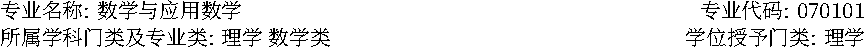
\includegraphics[width=\textwidth]{wku_programme_header.pdf}}{\textbf{Programme in Mathematical Sciences}\par\smallskip\hrule}
\vspace{18mm}
\begin{center}
\textbf{College of Science, Mathematics and Technology}\par
\medskip
\textbf{Wenzhou-Kean University}\par
\vspace{8mm}
\IfFileExists{WKU.png}{
\includegraphics[width=2.2055in,height=1.9055in]{WKU.png}}{\rule{0pt}{1.9055in}}\par
\vspace{25mm}
{\bfseries Parameter-Dependent Lie Symmetries\par
and Semi-Analytical Solutions\par
of Nonlinear PDEs\par}
\vspace{4mm}
Saint--Venant--Exner Case Studies\par
%{\small Lie-Invariant Reference Families and Targeted Corrections\par}
\vspace{3mm}
Undergraduate Dissertation (MATH 4890)
\end{center}
\vspace{10mm}
\noindent\begin{tabularx}{\textwidth}{@{}lX@{}}
\textbf{Student Name:} & \underline{Yihong Xiao}\\[4pt]
\textbf{Student ID:} & \underline{1308225}\\[4pt]
\textbf{Major:} & \underline{Mathematical Sciences}\\[-2pt]
 & \underline{(Data Analytics Option)}\\[4pt]
\textbf{Supervisor:} & \underline{Dr.\ Puneet Rana}\\[4pt]
\textbf{Review version:} & 26 November 2026
\end{tabularx}
\end{titlepage}
\hypersetup{pageanchor=true}
\setcounter{page}{2}
\chapter*{Author's Declaration}
\addcontentsline{toc}{chapter}{Author's Declaration}

\textbf{Draft declaration.}
I take responsibility for the final text, the attribution of sources and the
mathematical claims. I will verify that the submitted work and the disclosure
below meet the programme's requirements before signing.

\medskip
\noindent\textbf{AI assistance disclosure.}
ChatGPT drafted or revised explanatory prose in the introduction and the
chapter on Lie reduction, proposed the planar potential formulation and the
saddle determinant, and wrote first drafts of the benchmark code. Claude Opus 5.5
(in Cursor) helped design the SymPy Lie-reduction library for
$(1\text{--}3)+1$D SVE systems used in Chapter~\ref{ch:models} and implemented
the planar symbolic checks, the benchmark and the interval certifier of
Chapter~\ref{ch:computation}. Gemini drafted the prose of Chapters~3--5 from my
section-by-section decisions and styled the figures. Grok independently audited
the Python scripts. I checked every derivation and script by hand; formulas
first obtained with AI assistance are marked by footnotes, and every reported
number is produced by a committed script with a JSON record.

\vfill
\medskip

\noindent Date \rule[-.3ex]{3.5cm}{.4pt}\hfill Signature \rule[-.3ex]{5.5cm}{.4pt}

\clearpage


\begingroup\setstretch{1.0}\small
\chapter*{Abstract} %AlphaXiv-Skim format abstract
\addcontentsline{toc}{chapter}{Abstract}

\noindent\textbf{Goal.} Construct parameter-dependent Lie-invariant solutions of Saint--Venant--Exner (SVE) systems, extending them across declared physical domains and certifying approximations.

\medskip\noindent\textbf{Method.} Following the 2026 SVE symmetry and similarity-reduction method, we distinguish the printed scalar from its physically compatible counterpart. Determining kernels describe parameter strata; regular and Briot--Bouquet constructions describe reduced solution branches. A two-field planar potential formulation retains the three model parameters $m,K,G$. Exact reconstruction, analytic continuation, and interval-certified classical and learned profiles share one acceptance framework.

\medskip\noindent\textbf{Result.} The positive $(1+1)$ charts admit classical point-symmetry classification for every real $m\ge1$. The exponent $m=3$ adds a scaling, and $m=1$ adds a boost only to the printed scalar. Bed-drift solutions extend over their maximal positive-velocity interval. In the planar model a parameter-dependent determinant identifies nondegenerate saddles; a separate exact swirl has a convex bed for $1\le m<2$. For a non-rotating river bend with HEC-RAS bed-slope ratios $K/G\in[2,10]$, the threshold $c_*$ has a closed form. On held-out parameters, interval barriers certify the transcritical branch on $r\in[0.9,1.1]$ for Chebyshev, PINN, random-feature and gated networks (\NumCertAGated{} each); on $r\in[0.5,2]$ the gated cell certifies \NumCertBGated{} tuples and the plain PINN \NumCertBPinn. Learned warm starts reduce correction work, but no end-to-end cost advantage of learning is established. A whole-domain drift control is certified at \NumDriftCert{} held-out pairs. Local Taylor, Laurent and saddle constructions supply existence and convergence; neither general IBVP solvability nor a universal learning advantage is claimed.

\medskip\noindent\textbf{Keywords}\quad Parameter-dependent Lie symmetries, jet bundles, invariant reduction, Saint--Venant--Exner systems, material reconstruction, singular branches, fixed-point defect, structure-constrained approximation.

\section*{Notations}
{\footnotesize
\renewcommand{\arraystretch}{1.01}
\begin{tabularx}{\linewidth}{@{}p{.30\linewidth}X@{}}
\toprule
Symbol & Meaning\\\midrule
$\mathcal E_1,\mathcal E_P,\mathcal E_L$ & 2022 Eulerian SVE~\cite{sve2022}, 2026 printed scalar~\cite{sve2026}, compatible Lagrangian scalar derived from $\mathcal E_1$\\
$\mathcal E_2,\mathcal E_{2\text{-}\mathrm{exch}}$ & Rotating planar model and cubic exchange control\\
$\Delta_{i,j}$ & Eulerian residual. $i=1,2$ refers to the 2022 and 2026 papers, and $j=1,2,3$ to water mass, momentum and bed evolution.\\
$t,x,s,\phi(t,s)$ & Time, Eulerian position, mass label, inverse mass-coordinate function, $x=\phi(t,s)$\\
$h,u,B,b,q_b$ & Depth, velocity, Eulerian bed and its expression in mass coordinates, porosity-adjusted sediment flux\\
$L_0,H_0,U_0,T_0$ & Horizontal, depth, velocity and time scales, $T_0=L_0/U_0$\\
$g_{\rm d},A_{g,i,\rm d},\epsilon_{\rm bed}$ & Dimensional gravity, empirical Grass bedload coefficient and bed porosity\\
$g,m,\kappa_i,\kappa$ & Scaled gravity, transport exponent, bedload coefficient of source $i$, common coefficient $\kappa=\kappa_1=\kappa_2$\\
$\mathsf C,f,K,G$ & Coriolis matrix, Coriolis rate, bedload and bed-slope coefficients\\
$\Omega,\omega,k_d,k_e,D_a$ & Rotation and swirl rates, deposition and entrainment rates, mobile-load diffusivity\\
$Q_X,\mathscr D_\mu$ & Invariant-surface characteristic and on-shell determining operator\\
$F,p,L(z),I_0$ & Material profile, its derivative, common-scaling leading coefficient and first integral\\
$V,W,\Delta_c,\mathbf J_*$ & Radial and azimuthal velocities, radial leading coefficient, critical-point Jacobian\\
$c,C_j$ & Uniform bed drift and constants from ODE integration\\
$\mathcal T,\Lambda,\varpi$ & Profile fixed-point operator, contraction bound and prescribed trace\\\bottomrule
\end{tabularx}}
\endgroup
\clearpage
\tableofcontents
\clearpage
\pagenumbering{arabic}

\chapter{Introduction}\label{ch:introduction}
This dissertation follows the infinitesimal generators, one-dimensional subalgebra selection, and similarity reductions of Paliathanasis, Leon and Leach~\cite{sve2026}, together with the classical geometric foundations~\cite{olver,oliveri}. My motivation is mathematical: parameter changes can alter admitted symmetry directions, while singularities of a reduced equation can alter the existence of its solutions. I study these two mechanisms separately and use them to guide the construction, continuation and approximation of physically reconstructible profiles.

The Saint--Venant--Exner equations couple shallow-water motion with changes of the sediment bed. The HEC-RAS technical reference~\cite[Sec.~2.9, Eq.~(2-46)]{hecras2019} includes a slope-dependent bed-change term. It motivates retaining bed-slope effects in the planar reference model; the present idealized equations are not a reconstruction or calibration of HEC-RAS.

The first discriminant is the rank of a determining operator, which governs available group actions. The second is a vanishing coefficient in a reduced equation, which governs local solvability. We distinguish the printed material scalar $\mathcal E_P$ from the compatible equation $\mathcal E_L$ and reconstruct the Eulerian fields through a mass-coordinate inverse and a closed bed form. A planar potential formulation adds a spatial variable, a second unknown function, and a bed-slope parameter within a specified vorticity and circulation class.

The aim is an exact solution on its admissible domain whenever possible. Otherwise local analytic branches and their continuation provide the reference. Learning supplies candidate coefficients or profiles on the quotient; classical methods are independent controls. A continuous certificate, when available, is distinct from a sampled residual. General initial-boundary value problems, shocks and full planar group classification are outside the theorem scope.

\paragraph{Scope and overview.}
Chapter~\ref{ch:models} establishes the parameter-to-algebra map and reduction. Chapter~\ref{ch:continuation} develops the higher-dimensional model and its critical branches. Chapter~\ref{ch:computation} gives global reference solutions, continuation and parameter-conditioned approximation; the final chapter separates proved results from empirical findings. Figures~\ref{fig:workflow} and~\ref{fig:defect-workflow} show the reasoning chain.

\clearpage
\begin{figure}[!ht]\centering
\begin{tikzpicture}[
  flowbox/.style={draw=ink!65,fill=ink!4,rounded corners=2pt,text width=12.7cm,align=center,inner sep=5pt,font=\small},
  branch/.style={flowbox,text width=5.95cm,minimum height=1.05cm},
  route/.style={-{Latex[length=1.8mm]},draw=ink,line width=.8pt}]
\node[flowbox] (pde) {\textbf{Dimensionless SVE equations:} $\mathcal E_1,\ \mathcal E_P$};
\node[branch,below=5mm of pde.south west,anchor=north west] (lag)
 {Mass coordinates $x=\phi(t,s)$\quad (\S\ref{sec:physical-models})\\
 $\mathcal E_1\longrightarrow\mathcal E_L$};
\node[branch,below=5mm of pde.south east,anchor=north east] (plan)
 {Planar rotation and exchange\\
 $\mathcal E_2,\ \mathcal E_{2\text{-}\mathrm{exch}}$ (Ch.~\ref{ch:continuation})};
\draw[route] ([xshift=-3.2cm]pde.south)--(lag.north);
\draw[route] ([xshift=3.2cm]pde.south)--(plan.north);
\node[flowbox,below=19mm of pde] (lie)
 {\textbf{Find admitted generators} (\S\ref{sec:classification})\\
 $\mathscr D_\mu X=0$ with symbolic $m$: pivot minor and resonances, each candidate decided exactly};
\draw[route] (lag.south)--([xshift=-3.2cm]lie.north);
\draw[route] (plan.south)--([xshift=3.2cm]lie.north);
\node[flowbox,below=4mm of lie] (reduce)
 {\textbf{Reduce by invariant graphs} (\S\ref{sec:lie-tools})\\
 $Q_X=0$ on orbit chart $(z,v)$; accept if $\Delta=\mathsf M(z,v)\,\mathcal E[F](z)$, $\det\mathsf M\ne0$};
\draw[route] (lie)--(reduce);
\node[branch,below=5mm of reduce.south west,anchor=north west] (regular)
 {Regular profile equations\\ Invertible leading matrix};
\node[branch,below=5mm of reduce.south east,anchor=north east,fill=warm!6]
 (singular) {Singular profiles\\ Compatibility and adapted chart};
\draw[route] ([xshift=-3.2cm]reduce.south)--(regular.north);
\draw[route] ([xshift=3.2cm]reduce.south)--(singular.north);
\end{tikzpicture}
\caption[Analytical layer]{A change of coordinates expresses the physical equations in suitable variables. Lie invariance then reduces their independent variables. Parameter strata select the generators; profile singularities govern solvability.}
\label{fig:workflow}
\end{figure}

\begin{figure}[!ht]\centering
\begin{tikzpicture}[
  flowbox/.style={draw=ink!65,fill=ink!4,rounded corners=2pt,text width=12.7cm,align=center,inner sep=5pt,font=\small},
  branch/.style={flowbox,text width=5.95cm,minimum height=1.2cm},
  route/.style={-{Latex[length=1.8mm]},draw=ink,line width=.8pt}]
\node[flowbox] (data) {\textbf{Reduced equation and prescribed traces} (\S\ref{sec:records})};
\node[branch,below=5mm of data.south west,anchor=north west] (analytic)
 {Analytical and classical profiles\\ Closed forms, Taylor, Laurent, Chebyshev};
\node[branch,below=5mm of data.south east,anchor=north east] (learn)
 {Grey-box learning\\ Trace-exact gated residual cell};
\draw[route] ([xshift=-3.2cm]data.south)--(analytic.north);
\draw[route] ([xshift=3.2cm]data.south)--(learn.north);
\node[branch,below=4mm of analytic,fill=teal!6] (bound)
 {Continuous certificates\\ Series bounds and integral defect};
\node[branch,below=4mm of learn,fill=warm!6] (sample)
 {Sampled comparison\\ Held-out field errors and residuals};
\draw[route] (analytic)--(bound);
\draw[route] (learn)--(sample);
\node[flowbox,anchor=north] (recovery) at ($(bound.south)!0.5!(sample.south)+(0,-.5)$)
 {\textbf{Recover physical fields and substitute into the governing equations}};
\draw[route] (bound.south)--([xshift=-3.2cm]recovery.north);
\draw[route,dashed] (sample.south)--([xshift=3.2cm]recovery.north);
\end{tikzpicture}
\caption[Computational layer]{Chapter~\ref{ch:computation} establishes series convergence and continuous error bounds, and certifies the river-bend branch for classical and learned candidates (\S\ref{sec:comparison}); the tank polynomial replay is kept as a historical control (\S\ref{sec:replay}).}
\label{fig:defect-workflow}
\end{figure}

\chapter{SVE Models and Parameter-Dependent Reduction}\label{ch:models}
\section{Physical models and parameters}\label{sec:physical-models}

We start with the following two equations on positive-depth and positive-velocity charts. All fields and coefficients are dimensionless.

\paragraph{Eulerian system $\mathcal E_1$.} Equations (1)--(4) of the 2022 paper, \emph{Lie Symmetry Analysis of the One-Dimensional Saint--Venant--Exner Model}~\cite{sve2022}, give
\begin{equation}\label{eq:E}
\mathcal E_1:\quad
 \begin{cases}
 \Delta_{1,1}(t,x)=h_t+(hu)_x=0,\\
 \Delta_{1,2}(t,x)=u_t+uu_x+g(h+B)_x=0,\\
 \Delta_{1,3}(t,x)=B_t+\kappa_1(u^m)_x=0 .
 \end{cases}
\end{equation}

\paragraph{Printed scalar $\mathcal E_P$.} Equation (7) of the 2026 paper, \emph{Lie Symmetries and Similarity Solutions for a Shallow-Water Model with Bed Elevation in Lagrange Variables}~\cite{sve2026}, gives, for the unknown function $\phi(t,s)$ with $\phi_s,\phi_t>0$,
\begin{equation}\label{eq:P}
 \mathcal E_P[\phi](t,s)=D_t\left(\phi_s\phi_{tt}
       -g\frac{\phi_{ss}}{\phi_s^2}\right)
       -gm\kappa_2 D_s\left(\frac{\phi_t^{m-1}\phi_{ts}}{\phi_s}\right)=0.
\end{equation}

Here $D_t,D_s$ denote total derivatives with respect to $t,s$. For $\Delta_{i,j}$, $i=1,2$ identifies the source paper and $j=1,2,3$ the balance. With common scales and exponent, the two Eulerian systems differ at most in their bedload coefficients: $\Delta_{2,3}(t,x)=B_t+\kappa_2(u^m)_x$. Since the 2026 paper writes its flux derivative with $\beta=m\kappa_2$, we use $\kappa_i$ for both sources. Throughout the comparison we fix the same dimensionless parameters, $\kappa_1=\kappa_2=\kappa>0$, so $\Delta_{2,j}=\Delta_{1,j}$ for all $j$. The compatible Lagrangian scalar $\mathcal E_L$ will be derived from $\mathcal E_1$ below.

\paragraph{Physical interpretation.}
At horizontal position $x$ and time $t$, $B$ is the bed elevation from a fixed datum, $h>0$ the water depth and $u$ the depth-averaged velocity; $B+h$ is the surface elevation. The three balances in \eqref{eq:E} describe water mass with flux $hu$, acceleration due to the free-surface slope, and bed evolution due to sediment transport. The original conservative momentum residual $h\Delta_{1,2}+u\Delta_{1,1}$ gives the primitive equation when continuity holds on $h>0$.
The reference system uses hydrostatic, depth-averaged shallow-water flow on a horizontal scale large compared with the depth. Large Reynolds numbers motivate neglecting bulk viscosity. Omitting bed drag is a separate assumption about boundary stress~\cite{fernandez2017}. The shallow-water balances also omit dispersive corrections.

\paragraph{Nondimensionalization and the transport parameters.}
Let $L_0,H_0,U_0>0$ be horizontal, depth and velocity scales and $T_0=L_0/U_0$. Subscript $\mathrm d$ denotes dimensional quantities. With empirical Grass coefficient $A_{g,i,\rm d}$ in source $i$ and bed porosity $\epsilon_{\rm bed}\in[0,1)$, the effective flux is $q_{b,i,\rm d}=A_{g,i,\rm d}u_{\rm d}^m/(1-\epsilon_{\rm bed})$.
\[
 \begin{gathered}
 (x,\phi)=(x_{\rm d},\phi_{\rm d})/L_0,\quad
 t=t_{\rm d}/T_0,\quad (h,B,b,a)=(h_{\rm d},B_{\rm d},b_{\rm d},a_{\rm d})/H_0,\\
 (u,\mathbf w)=(u_{\rm d},\mathbf w_{\rm d})/U_0,\quad
 s=s_{\rm d}/(H_0L_0),\quad q_{b,i}=q_{b,i,\rm d}/(H_0U_0).
 \end{gathered}
\]
\begin{equation}\label{eq:dimensionless-params}
 g=\frac{g_{\rm d}H_0}{U_0^2},\qquad
 \kappa_i=\frac{A_{g,i,\rm d}U_0^{m-1}}{(1-\epsilon_{\rm bed})H_0},\quad
 q_{b,i}(u)=\kappa_i u^m\qquad(i=1,2).
\end{equation}
The units of $A_{g,i,\rm d}$ are $\mathrm{length}^{2-m}\mathrm{time}^{m-1}$. Both sources report the empirical range $1\le m\le4$~\cite{sve2022,sve2026}. We study the mathematical range $m\in[1,\infty)$, keeping $g,\kappa>0$ fixed while classifying each exponent. For $u>0$, $u^m=\exp(m\log u)$ is defined for every real $m$. At $m=0$ the flux is constant and the bed equation decouples from the velocity; for $0<m<1$ its derivative $mu^{m-1}$ is singular at $u=0$. We restrict the present theorem to $m\ge1$; behavior on $0\le m<1$ is a separate question.

\paragraph{Planar extension.}
Compared with $\mathcal E_1$, $\mathcal E_2$ uses horizontal vectors $\mathbf x=(x,y)$, $\mathbf w=(u,v)$ and adds Coriolis acceleration $\mathsf C\mathbf w=f\mathcal J\mathbf w$, where $\mathcal J(u,v)=(-v,u)$, and bed-slope transport with coefficient $G$~\cite{chesnokov,fernandez2017}. For general $m\ge1$, $K=\kappa=K_{\rm d}U_0^{m-1}/H_0$ and $G=G_{\rm d}U_0^{m-2}/L_0$ when the dimensional flux is written $|\mathbf w_{\rm d}|^{m-1}(K_{\rm d}\mathbf w_{\rm d}-G_{\rm d}\nabla B_{\rm d})$, with porosity absorbed. The exchange control uses $m=3$. The exchange variant adds centrifugal acceleration with frame rate $\Omega$ ($f=2\Omega$) and a mobile load $a=hC$, with concentration $C$, exchange rates $k_d,k_e$ and diffusivity $D_a$~\cite{parvin2026}. All rates, including $\omega$, scale by $T_0$ and $D_a=D_{a,\rm d}T_0/L_0^2$. The exchange closure is a model choice. Chapter~\ref{ch:continuation} specifies the planar system; Section~\ref{sec:exchange} defines the exchange control.

\section*{Eulerian to Lagrangian coordinates}
Let $s=s(t,x)$ represent a mass coordinate. We seek $s_x=h$ and $s_t=-hu$, so the compatibility condition $s_{xt}=s_{tx}$ is exactly $\Delta_{1,1}=0$. Equivalently, the one-form $h\,dx-hu\,dt$ is closed. On a simply connected local chart, it therefore has a primitive $s(t,x)$, unique up to a constant. Along $x(t)$ with $x'=u(t,x(t))$, the derivative of $s(t,x(t))$ vanishes. Thus $s$ labels a moving point of the depth-averaged flow.

Because $s_x=h>0$, the map $(t,x)\mapsto(t,s(t,x))$ has nonzero Jacobian $h$. The inverse function theorem supplies $x=\phi(t,s)$ with $\phi:\Omega_L\to\mathbb R$, where $\Omega_L$ is an open set in $\mathbb R^2$. Differentiating $s(t,\phi(t,s))=s$ with respect to $t$ and $s$ gives $s_t+s_x\phi_t=0$ and $s_x\phi_s=1$. Hence
\begin{equation}\label{eq:chain}
 \begin{gathered}
 h(t,\phi(t,s))=1/\phi_s,\qquad u(t,\phi(t,s))=\phi_t,\\
 \partial_x=\phi_s^{-1}D_s,\qquad
 \partial_t\big|_x=D_t-\frac{\phi_t}{\phi_s}D_s .
 \end{gathered}
\end{equation}
The derivative identities act on fields expressed in $(t,s)$. For example, define $b(t,s)=B(t,\phi(t,s))$. The chain rule gives
$b_t=B_t(t,\phi(t,s))+B_x(t,\phi(t,s))\phi_t$ and $b_s=B_x(t,\phi(t,s))\phi_s$. Consequently,
\[
 \boxed{B_t(t,\phi(t,s))=
 \underbrace{b_t}_{s\ \mathrm{fixed}}-
 \underbrace{\frac{\phi_t}{\phi_s}b_s}_{\mathrm{coordinate\ correction}}.}
\]
Here $\partial_t|_x$ keeps the physical position $x$ fixed; $D_t=\partial_t|_s$ differentiates along the moving mass label. This construction applies locally to any one-dimensional model with a source-free continuity equation and positive depth. Extra source terms change the compatibility condition, and in two spatial dimensions a single scalar mass label does not give an invertible spatial map.

For a fixed $\phi$, define two functions of $(t,s)$ by
\[
 \mathcal A[\phi](t,s)=\phi_s\phi_{tt}-g\phi_{ss}/\phi_s^2,\qquad
 T_m[\phi](t,s)=\phi_t^{m-1}\phi_{ts}/\phi_s .
\]
We abbreviate these as $\mathcal A(t,s)$ and $T_m(t,s)$. Under \eqref{eq:chain}, the Eulerian acceleration $u_t+uu_x$ becomes $\phi_{tt}$ and $h_x=-\phi_{ss}/\phi_s^3$. Multiplying momentum by $\phi_s$ and using the fixed-position bed derivative gives
\[
 \mathcal A(t,s)+gb_s=0,\qquad
 b_t-\frac{\phi_t}{\phi_s}b_s+m\kappa T_m(t,s)=0 .
\]
Eliminate $b$ by differentiating the two expressions for $b_s,b_t$ and equating $D_t b_s=D_s b_t$. This gives the compatible Lagrangian scalar
\begin{equation}\label{eq:M}
 \keyeq{\boxed{\mathcal E_L[\phi](t,s)=
 D_t\mathcal A-gm\kappa D_sT_m
 -D_s\left(\frac{\phi_t}{\phi_s}\mathcal A\right)=0.}}
\end{equation}
At the matched parameter $\kappa$, equation~\eqref{eq:P} omits the last term. In particular,
\[
 \boxed{\mathcal E_L[\phi]-\mathcal E_P[\phi]
 =-D_s\left(\frac{\phi_t}{\phi_s}\mathcal A\right).}
\]
The term is necessary because the Exner equation specifies the rate of change of the bed at fixed $x$. Using $b_t$ by itself replaces the Eulerian bed law by $B_t+uB_x+\kappa(u^m)_x=0$. The resulting scalar may thus have solutions and symmetries that are incompatible with the original Eulerian bed equation.\footnote{The source formula checks were set up with GPT assistance and checked by exact symbolic substitution in SymPy. See Appendix~\ref{app:audit} and the reproduction scripts.}

\begin{counterexample}\label{ex:p-neq-m}
For $\phi(t,s)=t+s+s^3/6$, we have $\phi_t=1$ and $\phi_s=q_1(s)=1+s^2/2>0$. Since $\mathcal A(t,s)=-gs/q_1(s)^2$ and $T_m=0$, the printed residual is $\mathcal E_{P}[\phi](t,s)=0$. The compatible residual is $\mathcal E_{L}[\phi](t,s)=-D_s(\mathcal A/\phi_s)=8g(2-5s^2)/(2+s^2)^4$ and equals $g$ at $s=0$.
\end{counterexample}

\begin{definition}[Physical reconstruction]\label{def:physical-reconstruction}
For a reduced or transformed solution function, physical reconstruction means recovering the original unknown fields through the inverse transformation and substituting them into all governing balances. For a solution $\phi(t,s)$ of $\mathcal E_L=0$, integrate the bed form for $b(t,s)$ and solve $x=\phi(t,s)$ for $s=s(t,x)$. The original fields are
\[
 h(t,x)=\frac{1}{\phi_s(t,s(t,x))},\quad
 u(t,x)=\phi_t(t,s(t,x)),\quad B(t,x)=b(t,s(t,x)).
\]
For an approximate profile, the same procedure evaluates the three residuals $\Delta_{1,j}$ of \eqref{eq:E}, provided the inverse is defined and a bed approximation is specified. A path integral of a nonclosed approximate bed form may depend on the path.
\end{definition}

\begin{proposition}[Local physical reconstruction]\label{prop:material}
On a simply connected material chart, let $\phi\in C^3(\Omega_L)$ with $\phi_s,\phi_t>0$. Every solution $\phi$ of $\mathcal E_{L}[\phi]=0$ determines a material bed elevation $b(t,s)$, unique up to an additive constant, through the exact one-form
\begin{equation}\label{eq:bed-form}
 \keyeq{db=\omega_{\mathcal E_{L}}=-\frac{\mathcal A(t,s)}{g}\,ds-\left(\frac{\phi_t\mathcal A(t,s)}{g\phi_s}+m\kappa T_m(t,s)\right)dt.}
\end{equation}
Since $\phi_s>0$, every point has a neighborhood on which $(t,s)\mapsto(t,\phi(t,s))$ is one-to-one. On that neighborhood, the lifted fields $h,u$ in \eqref{eq:chain} together with $B(t,\phi(t,s))=b(t,s)$ solve the Eulerian system $\mathcal E_1$.
\end{proposition}
\begin{proof}
Since $d\omega_{\mathcal E_{L}}=-\mathcal E_{L}[\phi](t,s)\,dt\wedge ds/g$, the form is closed. Its primitive on the simply connected chart recovers the two material balances. The continuity residual cancels under~\eqref{eq:chain}:

\[
 h_t+(hu)_x=\left(-\frac{\phi_{ts}}{\phi_s^2}+\frac{\phi_t\phi_{ss}}{\phi_s^3}\right)+\frac{1}{\phi_s}D_s\!\left(\frac{\phi_t}{\phi_s}\right)=0 .
\]
Since $\phi_s>0$, the inverse function theorem supplies a local lift, and the material balances become \eqref{eq:E}.
\end{proof}

\begin{remark}[Checks following from the scalar discrepancy]
Before eliminating a field, verify that the transformed balance uses the correct fixed variable. Before recovering physical fields, check positivity and local invertibility, and prescribe the bed constant. On a connected material domain the bed is single-valued precisely when every period $\oint_\Gamma\omega_{\mathcal E_L}$ vanishes; simple connectedness and closedness imply this. These checks distinguish admissible reductions from purely formal ones.
\end{remark}


\begin{figure}[!ht]\centering
\begin{tikzpicture}[x=1cm,y=1cm]
\node[box,text width=2.55cm,minimum height=1.03cm] (e) at (0,0)
 {\textbf{$\mathcal E_1$ in $(t,x)$}\\ Eulerian system};
\node[box,text width=3.0cm,minimum height=1.03cm] (l) at (4.55,0)
 {\textbf{Material system}\\ $(\phi,b)$ in $(t,s)$};
\node[box,text width=2.82cm,minimum height=1.03cm] (m) at (9.3,0)
 {\textbf{Scalar $\mathcal E_{L}$}\\ Closed bed form};
\node[warnbox,font=\small,text width=4.3cm,minimum height=.85cm] (p) at (4.55,-1.6)
 {\textbf{Printed $\mathcal E_{P}$}\\ $b_t+m\kappa T_m(t,s)=0$};
\draw[Latex-Latex,ink,thick] (e)--node[above,font=\scriptsize]{Mass map} (l);
\draw[Latex-Latex,ink,thick] (l)--node[above,font=\scriptsize]{Bed form} (m);
\draw[warr] (l)--node[right,font=\scriptsize]{Replace bed law} (p);
\end{tikzpicture}
\caption[Eulerian and material bed laws]{The mass map and bed primitive give a local correspondence on positive invertible charts with a chosen label origin and bed constant. The lower arrow changes the bed law to the advected form.}
\label{fig:material-chart}
\end{figure}

\section{Lie Reduction and Its Dependence on Parameters}\label{ch:lie}
Lie group reduction means expressing group-invariant solutions in fewer independent variables. Following the one-dimensional optimal system in~\cite{sve2026} and the foundations of Olver~\cite[Chs.~2--3]{olver} and Oliveri~\cite{oliveri}, I study how admitted generators vary with $\mu=(g,\kappa,m)$. Each fixed $\mu$ defines a separate PDE, with parameters constant under its symmetry action. Compared with fixed numerical coefficients, the additional task in the Python classification is to locate parameter values where $\ker\mathscr D_\mu$ changes, then solve and verify each branch. We first establish the common geometry.

\subsection{Jet coordinates, tangency and reduction}\label{sec:lie-tools}
Consider the compact representation $\Delta_\mu(x,U)=0$ of a PDE system, suppressing derivatives of $U$. Here $x=(x^1,\ldots,x^d)\in\Omega\subset\mathbb R^d$ contains the independent variables, including time, and $U:\Omega\to\mathbb R^r$ is the unknown vector-valued function. This extends the scalar $U=\phi$ in $\mathcal E_L$ to systems such as $U=(h,u,B)$ in $\mathcal E_1$. For order $n$ we write $\Delta_\mu(j^nU(x))=0$, where the jet $j^nU$ records $(x,U,(U^a_J))$ for multi-indices $J\in\mathbb N_0^d$, $1\le |J|\le n$, $1\le a\le r$. Each mixed partial occurs once. Full row rank of the residual differential makes the equation locus $\mathcal S_{\Delta_\mu}=\{q:\Delta_\mu(q)=0\}$ a submanifold. In point coordinates $U$ denotes the function values.

\begin{definition}[Classical point symmetry]
Let $\mathfrak X(E)$ denote the smooth vector fields on an open point chart $E\subset\Omega\times\mathbb R^r$. A smooth vector field $X\in\mathfrak X(E)$, with
$X=\sum_{i=1}^d\xi^i(x,U)\partial_{x^i}+\sum_{a=1}^r\eta^a(x,U)\partial_{U^a}$,
generates a local flow. It is a classical infinitesimal point symmetry if its prolongation is tangent to the regular equation locus, that is,
\[
 \pr^{(n)}X(q)\in T_q\mathcal S_{\Delta_\mu}
 \quad\Longleftrightarrow\quad
 \pr^{(n)}X(\Delta_\mu)(q)=0
 \qquad(q\in\mathcal S_{\Delta_\mu}).
\]
The prolongation is derived by differentiating the transformed graph: $\eta^a_\varnothing=\eta^a$ and $\eta^a_{J,i}=D_i\eta^a_J-\sum_j U^a_{J,j}D_i\xi^j$, where $D_i$ is the total derivative in $x^i$ and $J$ indexes derivatives~\cite[Chs.~2--3]{olver}. Its characteristic $Q_X^a=\eta^a-\sum_i\xi^i U_i^a$ measures the difference between the vertical motion and that required by graph tangency.
\end{definition}

Choose a finite-dimensional subalgebra $\mathfrak h$ of admitted generators $X_j=(\xi_j,\eta_j)$ with projectable coefficients $\xi_j(x)$. An invariant graph satisfies $Q_{X_j}=0$ for every generator. In a regular neighborhood assume the ranks of the base vectors $\xi_j$ and the point vectors $(\xi_j,\eta_j)$ are constant and equal to $k$. Figure~\ref{fig:orbit-geometry} illustrates the local section $x_\Sigma(z)$ with $d-k$ independent coordinates and the extension of a profile $F$ to an invariant graph $U=\ell[F]$. Define the reduced residual by
\begin{equation}\label{eq:reduction-map}
 \big(\mathcal R_{\mathfrak h}[\Delta](F)\big)(z)
 =c_\Sigma(z)\Delta(j^n\ell[F](x_\Sigma(z))),\quad c_\Sigma(z)\ne0.
\end{equation}
\begin{proposition}[Local reduction]\label{prop:regular-reduction}
On a regular jet chart and under these equal-rank and transverse-section hypotheses, the reduced solutions correspond locally to invariant solutions of the parent PDE. If $k=d-1$, the reduced system has one independent variable.
\end{proposition}
\begin{proof}
The equal ranks make the point-to-base orbit projection locally invertible along each orbit. The section fixes the local invariant extension. Prolonged symmetry flows preserve the equation locus, so the residual vanishes on the extension precisely when it vanishes on the section; multiplication by $c_\Sigma\ne0$ preserves this condition.
\end{proof}
For example, the purely vertical bed shift has $Q^B_{\partial_B}=1$, so a graph invariant under that generator alone does not exist. Singular orbits, conditional symmetries and boundary data require separate checks~\cite{anderson2000}.

\paragraph{Computing the quotient in $d$ variables.}
In two variables one can solve for the invariant $z(t,x)$ directly; with more variables this inversion is the hard step, and it can be avoided. Take $k=d-1$ generators whose coefficients are affine in $(x,U)$, so that each flow is a matrix exponential. Start from the profile graph $(x_\Sigma(z),F(z))$ on the section and move it by the group:
$(x,U)=\exp(v_1X_1)\cdots\exp(v_{d-1}X_{d-1})\,(x_\Sigma(z),F(z))$.
The group parameters $v$ and the section coordinate $z$ then serve as coordinates on the base, and $U=\ell[F](z,v)$ is the invariant graph written in them. Derivatives in $x$ follow from the chain rule $\partial_x=(\partial x/\partial(z,v))^{-\mathsf T}\partial_{(z,v)}$, so the invariants are never written explicitly. The reduction is accepted only after three exact identities: $Q_{X_j}[\ell[F]]=0$ for every $j$, $\det\partial x/\partial(z,v)\not\equiv0$, and
\begin{equation}\label{eq:weight-matrix}
 \Delta\big(j^n\ell[F]\big)(z,v)=\mathsf M(z,v)\,\mathcal E[F](z),\qquad \det\mathsf M\not\equiv0,
\end{equation}
with $\mathsf M$ free of $F$. This generalizes the scalar factor $c_\Sigma$ in \eqref{eq:reduction-map}: a rotation mixes the two momentum rows, so $\mathsf M$ is then a rotation matrix rather than diagonal. As a test independent of the SVE models, six seeded random scalar equations $u_t=\sum_i\nu_iu_{x_ix_i}+u\sum_ia_iu_{x_i}+\mu T$ in $(2+1)$D and $(3+1)$D, with a hidden coefficient or exponent in $T$, give eight strata with extra generators. Examples are a Galilean boost and a dilation at $\mu=0$ for $T=u$, and a dilation at $m=3$ for $T=\lambda u^m$. Each stratum reduces to an ODE through a closed subalgebra containing an extra generator.

\begin{figure}[!ht]\centering
\begin{tikzpicture}[x=1cm,y=1cm,
  panel/.style={anchor=west,font=\small\bfseries},
  tag/.style={font=\scriptsize,inner sep=2pt}]
\node[panel] at (0,2.74) {(a) Orbits and section};
\draw[arr] (.16,.33)--(4.55,.33) node[right,tag] {$t$};
\draw[arr] (.16,.33)--(.16,2.31) node[left,tag] {$s$};
\draw[authorblue,densely dashed,thick] (1.842,.33)--(1.842,2.27);
\node[tag,text=authorblue,anchor=south] at (1.842,2.28) {$\Sigma:\ t=t_*$};
\foreach \level/\idx in {.78/1,1.34/2,1.90/3}{
  \draw[teal,thick,domain=1.03:2.44,samples=46,variable=\u]
    plot ({.45+2.32*(\u-1)},{.33+\level/(\u*\u)});
  \draw[tarr,domain=1.74:2.08,samples=13,variable=\u]
    plot ({.45+2.32*(\u-1)},{.33+\level/(\u*\u)});
  \filldraw[fill=white,draw=authorblue,thick]
    (1.842,{.33+\level/(1.6*1.6)}) circle (1.55pt);
}
\node[tag,anchor=west,text=teal!80!ink,align=left] at (2.39,1.71)
  {Orbit label\\$\sigma=st^2$};
\node[tag,anchor=west] at (.15,.02) {$F(\sigma)=\phi(t_*,\sigma/t_*^2)$ on $\Sigma$};

\draw[ink!25] (4.98,-.07)--(4.98,2.62);
\node[panel] at (5.28,2.74) {(b) Two tangency tests};
\node[box,anchor=west,text width=5.70cm,font=\scriptsize,align=left,inner sep=4.5pt]
  (eqtest) at (5.35,2.11)
   {\textbf{Preserve the equation locus}\\
    $\pr^{(n)}X(\Delta)=0$ on $\Delta=0$};
\node[mlbox,anchor=west,text width=5.70cm,align=left,inner sep=4.5pt]
  (graphtest) at (5.35,1.10)
   {\textbf{Require an invariant graph}\\$Q_X=0$; for $Y_5$, this gives $\phi=F(st^2)$.};
\draw[arr] (graphtest.south)--($(graphtest.south)+(0,-.20)$);
\node[tag,anchor=north,align=center] at (8.34,.45)
  {Substitute the invariant graph in $\Delta$;\\
   evaluate on $\Sigma$ to get an ODE in $\sigma$.};
\end{tikzpicture}
\caption[Orbit section and the two tangency tests]{The section $\Sigma$ meets each displayed $Y_5$-orbit once. Its intersections, labelled by $\sigma=st^2$, represent the local quotient. Extending the trace $F$ along these orbits gives the invariant graph. The point field must be tangent to the graph; its prolongation must preserve the equation locus. The latter is why a reduced residual that vanishes on the section vanishes along the invariant extension.}
\label{fig:orbit-geometry}
\end{figure}

\section{Determining equations and the classification}\label{sec:classification}

For each fixed $\mu$ the on-shell determining operator $\mathscr D_\mu X=(\pr^{(n)}X\Delta_\mu)|_{\Delta_\mu=0}$ is linear in the coefficient functions of $X$. We eliminate the leading jet on a regular chart and split the prolonged identity by the remaining free jets. The splits force $\tau=\tau(t)$, $\xi=\xi(s)$ and an affine $\eta$, so the smooth problem collapses to a finite linear system $A_i(m)a=0$ for the slopes, with $m$ kept symbolic. Every resulting generator is then substituted into the full prolonged equation.\par
\begin{table}[!ht]\centering\small
\begin{tabularx}{\linewidth}{@{}lXll@{}}
\toprule
Equation & Basis present for all $m\ge1$ & Add at $m=1$ & Add at $m=3$\\\midrule
$\mathcal E_1$ & $X_1=\partial_t,\ X_2=\partial_x,\ X_3=\partial_B$,\newline
 $X_4=t\partial_t+x\partial_x$ & none & $X_5$\\
$\mathcal E_{L}$ & $Y_1=\partial_t,\ Y_2=\partial_\phi,\ Y_3=\partial_s$,\newline
 $Y_4=t\partial_t+s\partial_s+\phi\partial_\phi$ & none & $Y_5$\\
$\mathcal E_{P}$ & $Y_1,Y_2,Y_3,Y_4$ & $Y_6=t\partial_\phi$ & $Y_5$\\\bottomrule
\end{tabularx}
\[
 X_5=t\partial_t-u\partial_u-2h\partial_h-2B\partial_B,\qquad
 Y_5=t\partial_t-2s\partial_s .
\]
\caption{Generators on the positive charts. In the $\mathcal E_{L}$--$\mathcal E_1$ correspondence, indices $1,2,4,5$ give corresponding actions, with $5$ restricted to $m=3$. The bed constant and the mass-label origin are independent gauges.}
\label{tab:algebras}
\end{table}

\begin{theorem}[Point algebras of $\mathcal E_1$, $\mathcal E_{P}$, and $\mathcal E_{L}$]\label{thm:class}
For fixed $g,\kappa>0$ and any real $m\ge1$, the local smooth point-symmetry algebras of $\mathcal E_1$ (on $h,u>0$) and of $\mathcal E_{P}$ and $\mathcal E_{L}$ (on $\phi_t,\phi_s>0$) are precisely those listed in Table~\ref{tab:algebras}. Each algebra has dimension four except at the indicated exceptional exponents, where a single generator is added.
\end{theorem}
The four generic directions and the cubic extension were reported in~\cite{sve2022,sve2026}; Table~\ref{tab:algebras} corrects the former scaling and adds the printed scalar's linear-exponent boost. Appendix~\ref{app:proofs} proves the stated classification. A computation need only verify the generators it uses.

\begin{theorem}[Parameter-to-symmetry map and constant-rank continuation]\label{def:parameter-symmetry}
For $\mu=(g,\kappa,m)\in(0,\infty)^2\times[1,\infty)$, let $\mathcal G_i(\mu)=\ker\mathscr D_{i,\mu}$ denote the admitted point algebra for model $i\in\{1,P,L\}$. With the ordered candidate generators in Table~\ref{tab:algebras}, Theorem~\ref{thm:class} identifies a coefficient vector $a$ with $X=\sum_i a_iX_i$ or $Y=\sum_i a_iY_i$. The complete remaining constraints are
\begin{equation}\label{eq:parameter-kernel}
 \keyeq{A_1(m)=A_L(m)=(0,0,0,0,m-3),\quad
 A_P(m)=\begin{pmatrix}0&0&0&0&m-3&0\\0&0&0&0&0&m-1\end{pmatrix}.}
\end{equation}
Thus the kernel of $A_i(m)$ represents $\mathcal G_i(\mu)$ in its generating basis. For instance $m=5/2$ and $m=2$ give the same algebra. The family $\{(\mu,a):A_i(m)a=0\}$ has analytic defining equations and fibers of varying dimension. For any analytic finite determining matrix on a constant-rank analytic parameter stratum, its kernels form a local analytic vector bundle, and kernel dimension is upper semicontinuous on the whole parameter set. At a rank drop the exact kernel cannot be continuous in the gap topology along an approaching higher-rank stratum.
\end{theorem}
\begin{proof}
For rank $k$, select a nonzero $k$-minor and permute rows and columns to put it in a block $A_{11}$. The remaining variables are free, and the pivot variables equal $-A_{11}^{-1}A_{12}$ times them. The other rows impose no further restrictions on the constant-rank stratum. This gives an analytic frame. Nonvanishing minors make rank lower semicontinuous; hence kernel dimension is upper semicontinuous. For the three models, Theorem~\ref{thm:class} identifies the finite kernel exactly. In particular $(m-3)a_5=0$ and, for $\mathcal E_P$, $(m-1)a_6=0$ exclude continuation of the exceptional directions as nonzero exact extra generators off their strata. Approximate symmetries are not needed for this conclusion.
\end{proof}
The one-dimensional subalgebras are the lines $\mathbb P(\mathcal G_i(\mu))$. The parameter map is used with \eqref{eq:reduction-map} by selecting a projectable admitted line on a regular chart with equal positive base and point ranks. Adjoint equivalence only matters when inequivalent representatives are sought~\cite{olver}.

\subsection{Tools for parameter stratification}\label{sec:exceptional}
\paragraph{The cubic scaling at $m=3$.}
Under the dilation $Y_5=t\partial_t-2s\partial_s$, the material terms $D_t\mathcal A$ and $D_s(\phi_t\mathcal A/\phi_s)$ both carry weight $-1$, whereas $D_s T_m$ carries weight $2-m$; these weights coincide precisely when $m=3$. In Eulerian variables, the water mass and momentum balances are homogeneous under $X_5$, while the prolonged action on the bed law leaves the on-shell residual $(3-m)\kappa(u^m)_x$, which vanishes only at $m=3$.

Equivalently, consider the three-parameter scaling equivalence group $(t,x,u,h,B)\mapsto(Tt,Lx,(L/T)u,\chi h,\chi B)$ with $T,L,\chi>0$. Because the inertial terms scale by $L/T^2$ and $B_t$ scales by $\chi/T$, the dimensionless parameters transform as
\begin{equation}\label{eq:parameter-action}
 \widetilde g=g(L/T)^2/\chi,\qquad
 \widetilde\kappa=\kappa\chi(L/T)^{1-m},\qquad
 \keyeq{\widetilde{g\kappa}=g\kappa(L/T)^{3-m}.}
\end{equation}
For $m\ne3$, both positive coefficients can be normalized to unity. At $m=3$, $g\kappa$ is invariant and the stabilizer satisfies $\chi=(L/T)^2$. Its two generators are the common dilation $X_4$ and the extra scaling $X_5$. Indeed, $T=e^{a+b}$, $L=e^a$, $\chi=e^{-2b}$ give the flow of $aX_4+bX_5$.

\paragraph{The linear exponent at $m=1$.}
At $m=1$, a Galilean boost $x\mapsto x+\epsilon t$ reads $\phi\mapsto\phi+\epsilon t$ in material coordinates. It leaves both $\mathcal A$ and $T_1=\phi_{ts}/\phi_s$ invariant, and therefore generates the extra symmetry $Y_6=t\partial_\phi$ of $\mathcal E_{P}$. In $\mathcal E_{L}$, however, the fixed-position bed derivative contributes the extra term $-\epsilon D_s(\mathcal A/\phi_s)$ under the boost; because this term contains the free jet $\phi_{tts}$, it obstructs $Y_6$ from being a symmetry of $\mathcal E_{L}$.

\paragraph{Locating exceptional exponents.}
In the finite affine search, splitting powers $u^{am+b}$ is valid off coincidences $(a-a')m=b'-b$ on $u>0$, provided the coefficients do not depend on $u$. A nonzero generic maximal minor detects possible rank drops; add the power coincidences and any denominator exceptions and re-evaluate the original determining equations at each candidate. Table~\ref{tab:strata} records the affine search, not its extension to arbitrary coefficient functions. Appendix~\ref{app:proofs} supplies the smooth classifications.
\begin{table}[!ht]\centering\small
\begin{tabular}{@{}lllll@{}}\toprule
Model & Pivot-minor factors & Resonances & Jumps & Extra generators\\\midrule
$\mathcal E_1$ & $m,\ m-1,\ m-3$ & $1,2,3$ & $m=0,3$ & $X_5$ at $m=3$\\
$\mathcal E_P$ & $m,\ m-1,\ m-3$ & $0,\ldots,4$ & $m=0,1,3$ & $Y_6$ at $m=1$; $Y_5$ at $m=3$\\
$\mathcal E_L$ & $m,\ m-3$ & $0,\ldots,4$ & $m=0,3$ & $Y_5$ at $m=3$\\\bottomrule
\end{tabular}
\caption[Automatically detected parameter strata]{Affine determining search with symbolic $m$. Generic kernels are four-dimensional; every candidate is decided by exact specialization.}
\label{tab:strata}
\end{table}

\paragraph{Implementation.}
All symbolic computations use \texttt{SymPy} alone, because I do not work with Mathematica or Maple. Claude Opus 5.5 helped design this small Lie-reduction library for SVE systems with one to three spatial variables. I checked the scripts by hand so that every step stays exact: each generator is substituted into the full prolonged equation, and each reduced equation is accepted only through the identities \eqref{eq:weight-matrix}.

\subsection{Lie formulation of the bed-drift family}\label{sec:arbitrary-flux}
Replace $\kappa u^m$ in $\mathcal E_1$ by any $Q\in C^2(I)$, where $I\subset(0,\infty)$ is an open velocity interval. The system $\mathcal E_1[Q]$ retains both water balances and has $B_t+D_xQ(u)=0$. Berthon et al.~\cite[Prop.~2.1 and Eqs.~(10)--(12)]{berthon2012} derived a constant-discharge bed-drift solution for a family of sediment laws. Here we identify the common generating symmetry and give the local inverse criterion for arbitrary $C^2$ velocity fluxes. The kernel $\mathcal G[Q]=\ker\mathscr D_Q$ contains $\partial_t,\partial_x,\partial_B$ because the equations are autonomous and use only derivatives of $B$. There is no need to classify other symmetries for the following reduction.
\begin{proposition}[Bed-drift reduction for a general velocity flux]\label{prop:general-flux}
For every such $Q$ and $g>0$, $T_\alpha=\partial_t+\alpha\partial_B$ is admitted for any $\alpha\in\mathbb R$. Its base and point orbit ranks equal one. The invariant graph is $u(t,x)=U(x)$, $h(t,x)=H(x)$ and $B(t,x)=Z(x)+\alpha t$. On $H,U>0$, the three integrated equations are
\begin{equation}\label{eq:general-flux}
 \keyeq{HU=C,\qquad U^2/(2g)+H+Z=E,\qquad
 Q(U(x))=Q(U_0)-\alpha(x-x_0).}
\end{equation}
Here $U(x_0)=U_0\in I$, $C>0$, and $E$ is the prescribed Bernoulli constant. If $Q'(U_0)\ne0$, there is a unique local $C^2$ profile for these data, with $H=C/U$ and $Z=E-H-U^2/(2g)$. If $Q$ is analytic, the profile is analytic. For $\alpha\ne0$ and $Q'(U_0)=0$, no $C^1$ profile passes through $U_0$.
\end{proposition}
\begin{proof}
Substitution gives $(HU)'=0$, $UU'+g(H'+Z')=0$, and $\alpha+Q'(U)U'=0$. Integrate to obtain \eqref{eq:general-flux}; the inverse function theorem applies at $Q'(U_0)\ne0$. At $Q'(U_0)=0$, the third equation forces $\alpha=0$ for any finite $U'$. Restoring the invariant graph satisfies every original balance.
\end{proof}
\paragraph{Maximal regular domain.}
For a connected interval $I_*$ on which $Q'\ne0$, $Q$ is one-to-one. The profile in Proposition~\ref{prop:general-flux} is defined on exactly the component containing $x_0$ of
\[
 \{x: Q(U_0)-\alpha(x-x_0)\in Q(I_*)\}.
\]
This is the maximal interval within that monotonic regular chart. For $Q(u)=\kappa u^m$, $\kappa>0$, $m\ge1$, the positive branch is
\begin{equation}\label{eq:global-drift}
 U(x)=\left(U_0^m-\alpha(x-x_0)/\kappa\right)^{1/m}.
\end{equation}
Its domain is the entire half-line where the base is positive ($\mathbb R$ for $\alpha=0$). For $\alpha\ne0$, $U\to0$ at the finite endpoint and $H=C/U\to\infty$; no extension with finite positive depth crosses that endpoint. Reconstruction holds for all real $t$ on this spatial chart. This establishes a global invariant family, not an arbitrary-data solution.

For $Q(u)=\kappa u^m$ ($m\ge1$), $Q'>0$ on the positive chart. For example, $Q(u)=e^u$ gives $U(x)=\log(e^{U_0}-\alpha(x-x_0))$ locally. Every nonconstant $C^2$ flux on a connected interval has a regular velocity; constant $Q$ admits steady profiles with $\alpha=0$. This guarantee is local to the autonomous velocity-flux SVE family. Other constitutive dependencies, forcing and boundary data require separate checks.

\subsection{One-dimensional reductions}\label{sec:reductions}
We use the bed-drift and travelling-wave translations, the common and cubic scalings, and the printed scalar's $m=1$ boost. Their reduced equations follow here and in Section~\ref{sec:common-scale}; the boost combination $Y_3+Y_6$ is used in Appendix~\ref{app:historical-comparison}. All require a chart compatible with the prescribed data.

\begin{example}[Cubic Eulerian reduction]\label{ex:x5}
At $m=3$ use the generator $X_5$ from Table~\ref{tab:algebras}. On $t>0$, its base rank and point rank are both one. Integrating the equations of the group flow gives
$(t,x,u,h,B)\mapsto(e^\varepsilon t,x,e^{-\varepsilon}u,e^{-2\varepsilon}h,e^{-2\varepsilon}B)$.
The invariants are $x,tu,t^2h,t^2B$. Solving $Q_{X_5}=0$ is equivalent to $tu_t=-u$, $th_t=-2h$, $tB_t=-2B$, so
\[
 u(t,x)=U(x)/t,\qquad h(t,x)=H(x)/t^2,\qquad B(t,x)=Z(x)/t^2.
\]
The residuals in \eqref{eq:E} become $t^{-3}[(HU)'-2H]$, $t^{-2}[U(U'-1)+g(H'+Z')]$ and $t^{-3}[\kappa(U^3)'-2Z]$, respectively. Multiplying each by its positive power of $t$ gives
\begin{equation}\label{eq:eulerian-cubic}
 \keyeq{(HU)'=2H(x),\quad U(x)(U'-1)+g(H'+Z')=0,\quad \kappa(U^3)'=2Z(x).}
\end{equation}
This is the map from a three-field PDE to three ODEs. The closed-form profile is derived in Section~\ref{sec:closed-forms}.
\end{example}

\begin{example}[Cubic material reduction]\label{ex:y5}
For $Y_5$ the characteristic is $Q_{Y_5}=2s\phi_s-t\phi_t$. Its flow is $(t,s,\phi)\mapsto(e^\varepsilon t,e^{-2\varepsilon}s,\phi)$. Thus $\sigma=st^2$ is constant along the base orbits (Figure~\ref{fig:orbit-geometry}), giving $\phi(t,s)=F(\sigma)$.
Writing $p(\sigma)=F'(\sigma)>0$ on $\sigma>0$, the derivatives are $\phi_t=2\sigma p/t$, $\phi_s=t^2p$, $\phi_{tt}=(2\sigma p+4\sigma^2p')/t^2$ and $\phi_{ts}=2t(p+\sigma p')$. Substitution gives
\begin{equation}\label{eq:cubic-terms}
 \mathcal A_\sigma(\sigma)=2\sigma p(\sigma)^2+4\sigma^2p(\sigma)p'-gp'/p(\sigma)^2,\quad
 \mathcal J_\sigma(\sigma)=8\sigma^2 p(\sigma)(p(\sigma)+\sigma p'),
\end{equation}
so that $\mathcal A(t,s)=\mathcal A_\sigma(\sigma)$ and $T_3(t,s)=t^{-3}\mathcal J_\sigma(\sigma)$. Since $tD_s((\phi_t/\phi_s)\mathcal A)=2(\sigma\mathcal A_\sigma)'$, normalizing by $t>0$ puts both cubic scalar reductions on a common footing:
\begin{equation}\label{eq:cubic-reduced}
 t\mathcal E_{P}[\phi](t,s)=2\sigma\mathcal A_\sigma'-3g\kappa\mathcal J_\sigma',
 \qquad t\mathcal E_{L}[\phi](t,s)=-2\mathcal A_\sigma(\sigma)-3g\kappa\mathcal J_\sigma'.
\end{equation}
Since $\partial_\phi$ commutes with $Y_5$, both reduced equations depend on $p(\sigma)=F'(\sigma)$.
\end{example}

\paragraph{Translation and travelling-wave profiles.}
For the general translation combination $\phi(t,s)=\gamma t+F(z)$ with $z=s-ct$, write $p(z)=F'(z)$ and $u_\gamma(p)=\gamma-cp$. On the positive chart $p(z),u_\gamma(p(z))>0$, direct substitution gives
\begin{align}
 \mathcal E_{L}[\phi](t,s)&=(L_{c,\gamma}(p(z))p')',&
 L_{c,\gamma}(p)&=\gamma(g/p^3-c^2)+gm\kappa c\,u_\gamma(p)^{m-1}/p,\notag\\
 \mathcal E_{P}[\phi](t,s)&=(L^{\mathcal E_{P}}_{c,\gamma}(p(z))p')',&
 L^{\mathcal E_{P}}_{c,\gamma}(p)&=c(-c^2p+g/p^2+gm\kappa u_\gamma(p)^{m-1}/p).
 \label{eq:tilted}
\end{align}
Indeed, $\mathcal A(t,s)=(c^2p(z)-g/p(z)^2)p'$ and $T_m(t,s)=-cu_\gamma(p(z))^{m-1}p'/p(z)$; in $\mathcal E_{L}$, the coefficient of $\mathcal A'$ combines with the advection factor to produce $-(\gamma\mathcal A/p)'$. These equations are in divergence form. Their integrated solutions and the corresponding physical fields are given in Section~\ref{sec:closed-forms}.

\section{Common-scaling profile equation}\label{ch:series}\label{sec:common-scale}
The common scaling gives the first integral used in Chapter~\ref{ch:computation}.
Consider the common-scaling reduction under $Y_4$, given by $\phi(t,s)=tF(z)$ with similarity variable $z=s/t$, derivative $p(z)=F'(z)$, and velocity $v_*(z)=F(z)-zp(z)$, on the positive chart $t,p(z),v_*(z)>0$. Abbreviating $L(z)=L_{\mathcal E_{L}}(z,F(z),p(z))$, substitution into \eqref{eq:M} gives an exact derivative:
\begin{equation}\label{eq:Lc}
 \keyeq{t^2\mathcal E_{L}[\phi](t,s)=(L(z)F'')'},\quad
 L_{\mathcal E_{L}}(z,F,p)=F(g/p^3-z^2)+gm\kappa z(F-zp)^{m-1}/p.
\end{equation}
This follows from $\mathcal A(t,s)=F''(z^2p(z)-g/p(z)^2)/t$ and $T_m(t,s)=-zv_*(z)^{m-1}F''/(tp(z))$. Integrating once yields the first integral $I_0=L(z)F''$, which is constant along any $Y_4$-invariant profile.

Where $L(z)\ne0$, $F'=p$, $p'=I_0/L(z)$ (see Section~\ref{sec:series-solvability}).

\chapter{Higher-Dimensional SVE and Analytic Branches}\label{ch:continuation}
Having established the Lie-reduction tools in Chapter~\ref{ch:models}, we complete the semi-analytical workflow on a planar model built from the Eulerian system~\cite{sve2022} and the material setting~\cite{sve2026} by adding one horizontal spatial dimension and cited bed-slope parameter ranges. Symbolic reduction leaves coupled radial ordinary differential equations that numerical and certified computation complete. Learning is reserved for reduced branches where closed forms fail and singular continuation is difficult.

\section{Planar model and potential formulation}\label{sec:annular-model}
We formulate the planar Saint--Venant--Exner system $\mathcal E_2$ on an annulus and establish its two-field potential form in a fixed vorticity and circulation class. On an annulus $r=|\mathbf x|>0$, with $g,K,G>0$, $f\ge0$, and real $m\ge1$, define $\mathcal E_2$ by
\begin{align}\label{eq:planar}
 h_t+\nabla\cdot(h\mathbf w)&=0,\notag\\
 \mathbf w_t+(\mathbf w\cdot\nabla)\mathbf w+g\nabla(h+B)+f\mathcal J\mathbf w&=0,\notag\\
 B_t+\nabla\cdot\mathbf Q&=0,\notag\\
 \mathbf Q&=|\mathbf w|^{m-1}(K\mathbf w-G\nabla B),
\end{align}
where $\mathcal J(u,v)=(-v,u)$ is the quarter-turn rotation; $f=0$ represents a non-rotating river bend and $f>0$ a rotating frame. The bed-slope transport term is motivated by~\cite{fernandez2017,hecras2019}; because $G>0$ introduces diffusion into the Exner balance, $\mathcal E_2$ is mixed hyperbolic--parabolic rather than purely first-order hyperbolic.

\begin{proposition}[Two-field potential formulation]\label{prop:potential}
Assume smooth fields on an annulus $r=|\mathbf x|>0$ with $h>0$, $|\mathbf w|>0$, zero absolute vorticity $\operatorname{curl}\mathbf w+f=0$, and fixed circulation $2\pi C_2$ of $\mathbf w+(f/2)\mathcal J\mathbf x$ around the hole. Set
\begin{equation}\label{eq:potential-lift}
 \mathbf w=\nabla\psi+\left(C_2/r-fr/2\right)\mathbf e_\theta,
 \qquad \Xi=\psi_t+\tfrac12|\mathbf w|^2+gh .
\end{equation}
Choosing the time gauge of the single-valued potential $\psi(t,x,y)$, the compatible equations for the two scalar unknowns $h$ and $\psi$ are
\begin{equation}\label{eq:potential-pde}
 \keyeq{\begin{aligned}
 h_t+\nabla\cdot(h\mathbf w)&=0,\\
 \Xi_t&=\nabla\cdot\left[|\mathbf w|^{m-1}(gK\mathbf w+G\nabla\Xi)\right].
 \end{aligned}}
\end{equation}
Together with $B=-\Xi/g$, they recover all Eulerian balances of~\eqref{eq:planar} in the stated flow class.
\end{proposition}
The proof is in Appendix~\ref{app:potential-proof}; the lift, the vector identity and the reverse recovery are also exact SymPy checks in \code{verify_planar.py}.

The physical scope of $\mathcal E_2$ is intentionally restricted: it assumes zero absolute vorticity, no bed friction, no secondary helical circulation, and a power-law sediment flux. Real channel bends---for instance the EPFL laboratory flume~\cite{zeng2008}, which has centreline radius $1.7$\,m and width $1.3$\,m (placing the inner and outer banks near $r\approx0.62$--$1.38$ in units of the centreline radius)---exhibit both bed friction and helical secondary flow, so $\mathcal E_2$ serves as a mathematical seed for computation rather than a calibrated river model. Bed friction is not added here because a drag force is not a gradient, which breaks both the potential formulation and the azimuthal first integral. Within this model, I reserve learning strictly for hard reduced tasks: the primary target is the non-rotating ($f=0$) bend saddle branch of Section~\ref{sec:saddle}, which has no closed form, passes through a singular transcritical crossing, retains the non-integer power law $|\mathbf w|^{m-1}$, and varies with three active parameters.

\section{Rank-two reduction and radial integrals}\label{sec:radial}
We reduce $\mathcal E_2$ by two commuting symmetries to a radial system in one independent variable. For $f\ge0$, the parent system~\eqref{eq:planar} admits horizontal rotations and uniform time--bed shifts:
\[
 R=-y\partial_x+x\partial_y-v\partial_u+u\partial_v,
 \qquad T_c=\partial_t+c\partial_B .
\]
Away from the origin, the projected fields $\partial_\theta$ and $\partial_t$ commute and have rank two. In the potential chart~\eqref{eq:potential-lift}, the corresponding generators are rotation in $(x,y)$ and $\partial_t-gct\partial_\psi$, which fixes $\psi=\Psi(r)-gct^2/2$ up to the bed datum. The Eulerian invariant graphs take the form
\[
 h=H(r),\qquad \mathbf w=V(r)\mathbf e_r+W(r)\mathbf e_\theta,
 \qquad B=Z(r)+ct .
\]
For $H,r>0$ and nonzero radial velocity $V$, the mass, azimuthal momentum, and Exner balances integrate directly to three radial first integrals:
\[
 rHV=C_1,\qquad rW+fr^2/2=C_2,\qquad rQ+cr^2/2=C_3 .
\]
Because $rW+fr^2/2$ is constant, this branch lies inside the circulation class of Proposition~\ref{prop:potential}. Figure~\ref{fig:bend} illustrates the annular-sector bend geometry, the orbits of $\partial_\theta$, the transversal section $\theta=0$, and a sampled radial profile at the EPFL flume scale.

\begin{figure}[!ht]\centering
\IfFileExists{figures/planar/fig_bend.tex}{\begin{tikzpicture}
  % Left: plan view of annular-sector river bend (r in [0.62, 1.38], opening 120 deg)
  \begin{scope}[shift={(0,0)}]
    \def\Rsc{2.15} % cm per unit dimensionless radius
    \pgfmathsetmacro\Rin{0.62*\Rsc}
    \pgfmathsetmacro\Rmid{1.00*\Rsc}
    \pgfmathsetmacro\Rout{1.38*\Rsc}

    % Shaded sector
    \fill[teal!8]
      (0:\Rin) arc[start angle=0, end angle=120, radius=\Rin]
      -- (120:\Rout) arc[start angle=120, end angle=0, radius=\Rout] -- cycle;

    % Inner and outer walls
    \draw[ink, line width=0.9pt]
      (0:\Rin) arc[start angle=0, end angle=120, radius=\Rin];
    \draw[ink, line width=0.9pt]
      (0:\Rout) arc[start angle=0, end angle=120, radius=\Rout];

    % Upstream boundary (theta = 120 deg)
    \draw[ink!55, densely dashed, line width=0.6pt] (120:\Rin) -- (120:\Rout);

    % Radial construction lines from centre O
    \draw[black!35, densely dotted] (0,0) -- (0:\Rin);
    \draw[black!35, densely dotted] (0,0) -- (120:\Rin);
    \fill[ink] (0,0) circle (1.2pt) node[below left, font=\scriptsize, inner sep=1.5pt] {$O$};
    \draw[black!45, line width=0.45pt] (0:0.52) arc[start angle=0, end angle=120, radius=0.52];
    \node[font=\scriptsize, text=black!65] at (60:0.78) {$120^\circ$};

    % Orbits of \partial_\theta (rotation R): 3 dashed concentric arcs with arrowheads
    \foreach \rad in {0.78, 1.00, 1.22}{
      \pgfmathsetmacro\rr{\rad*\Rsc}
      \draw[teal!85!ink, densely dashed, line width=0.65pt]
        (114:\rr) arc[start angle=114, end angle=6, radius=\rr];
      \draw[-{Latex[length=1.45mm, width=1.1mm]}, teal!85!ink, line width=0.65pt]
        (68:\rr) arc[start angle=68, end angle=48, radius=\rr];
    }

    % Downstream transversal section theta = 0
    \draw[warm, line width=1.35pt] (0:\Rin) -- (0:\Rout);
    \node[font=\scriptsize, text=warm, anchor=north, inner sep=2pt]
      at (0:{0.5*(\Rin+\Rout)}) {section $\theta=0$};

    % Radius tick marks along theta = 0
    \foreach \val/\lbl in {0.62/$0.62$, 1.00/$1$, 1.38/$1.38$}{
      \pgfmathsetmacro\xx{\val*\Rsc}
      \draw[ink, line width=0.5pt] (\xx, 0.06) -- (\xx, -0.06);
      \node[font=\tiny, text=ink, anchor=north] at (\xx, -0.35) {\lbl};
    }
    \node[font=\scriptsize, text=ink, anchor=west, inner sep=2pt] at (\Rout+0.04, 0.02) {$r$};

    % Orbit label cleanly above the bend
    \node[font=\scriptsize, text=teal!85!ink, align=center]
      at (68:{\Rout+0.50}) {orbits of $\partial_\theta$ (rotation $R$)};
  \end{scope}

  % Right: elevation profiles along section theta = 0 from profile_B.dat
  \begin{axis}[
    at={(4.65cm,-0.32cm)},
    scale only axis,
    width=6.6cm,
    height=3.65cm,
    xmin=0.62, xmax=1.38,
    ymin=-3.0, ymax=2.40,
    xtick={0.7, 0.85, 1.0, 1.15, 1.3},
    ytick={-3, -2, -1, 0, 1, 2},
    tick label style={font=\scriptsize},
    label style={font=\footnotesize},
    xlabel={$r$},
    ylabel={elevation},
    ylabel style={yshift=-2pt},
    xlabel style={yshift=2pt},
    axis line style={ink!70},
    tick style={ink!70},
    restrict x to domain=0.62:1.38,
    unbounded coords=jump,
    title style={font=\footnotesize, yshift=-3pt},
    title={section $\theta=0$ profile},
  ]
    % Reference bottom path for bed fill
    \path[name path=bot] (axis cs:0.62,-3.0) -- (axis cs:1.38,-3.0);

    % Bed Z_ref
    \addplot[ink, line width=1.0pt, name path=bed]
      table[x=r, y=Z_ref] {figures/planar/profile_B.dat};

    % Free surface H_ref + Z_ref
    \addplot[teal, line width=1.1pt, name path=surf]
      table[x=r, y=HZ_ref] {figures/planar/profile_B.dat};

    % Shaded bed and water column
    \addplot[ink!12] fill between[of=bed and bot];
    \addplot[teal!14] fill between[of=bed and surf];

    % Re-stroke curves cleanly over fills
    \addplot[ink, line width=1.0pt]
      table[x=r, y=Z_ref] {figures/planar/profile_B.dat};
    \addplot[teal, line width=1.1pt]
      table[x=r, y=HZ_ref] {figures/planar/profile_B.dat};

    % Centreline marker r = 1
    \draw[black!35, densely dotted, line width=0.55pt]
      (axis cs:1.0,-3.0) -- (axis cs:1.0,2.40);

    % Curve labels placed cleanly away from ticks and dotted line
    \node[font=\scriptsize, text=teal!90!black, anchor=south east, inner sep=1.5pt]
      at (axis cs:1.28, 1.62) {$H+Z$};
    \node[font=\scriptsize, text=ink, anchor=north, inner sep=1.5pt]
      at (axis cs:1.10, -0.06) {$Z$};

    % Depth H indicator at r = 1.24
    \draw[{Latex[length=1.1mm]}-{Latex[length=1.1mm]}, teal!80!ink, line width=0.55pt]
      (axis cs:1.24, -0.22) -- (axis cs:1.24, 1.54)
      node[midway, right, font=\scriptsize, inner sep=1.5pt] {$H$};

    % Time-bed drift T_c arrow next to the bed
    \draw[-{Latex[length=1.6mm]}, warm, thick]
      (axis cs:1.04, -2.55) -- (axis cs:1.04, -1.45);
    \node[font=\scriptsize, text=warm, anchor=west, align=left, inner sep=2pt]
      at (axis cs:1.06, -2.02) {$T_c=\partial_t+c\,\partial_B$\\[-1pt](bed drift)};
  \end{axis}
\end{tikzpicture}
}{\fbox{fig\_bend pending}}
\caption[Annular-sector bend geometry and radial section]{Left: annular-sector bend with orbits of $\partial_\theta$, the transversal section $\theta=0$, and the uniform bed drift $T_c$; the inner and outer bank radii $r\approx0.62$--$1.38$ follow the EPFL flume aspect ratio~\cite{zeng2008} purely as a geometric scale. Right: reference bed $Z$ and free surface $H+Z$ along $\theta=0$ for one stage-B parameter tuple (sampled DOP853 reference, $Z(1)=0$).}
\label{fig:bend}
\end{figure}

Since a constant net water flux $2\pi C_1$ crosses every concentric circle, $C_1\ne0$ models an open bend reach rather than an impermeable closed tank. Exact symbolic checks in \code{verify_planar.py} confirm that $R$ and $T_c$ are admitted for every $(m,K,G,f)$, so no parameter stratum enters this reduction and the only remaining singularities are those of the reduced ODE. Defining $S=V^2+W^2$ with $V=C_1/(rH)$, $W=C_2/r-fr/2$, and $Q=C_3/r-cr/2$, the radial flux relation $Q=S^{(m-1)/2}(KV-GZ')$ yields $P_Z(r,H)=(KV-Q/S^{(m-1)/2})/G$, $\Delta_c=gH-V^2$, and $N(r,H)=H(S/r+fW-gP_Z)$. Under these integrals, exact symbolic checks verify that the mass, azimuthal, and Exner residuals vanish identically, the radial momentum residual equals $(\Delta_c H'-N)/H$, and $N$ is homogeneous of degree zero in $(K,c,C_3,G)$: the reduced profile therefore depends only on $(m,\kappa,\gamma,f)$ with $\kappa=K/G$ and $\gamma=c/G$. The reduced radial system is
\begin{equation}\label{eq:DN}
 \keyeq{\Delta_c H'=N,\qquad Z'=P_Z.}
\end{equation}

\section{Analytic crossing of a radial critical point}\label{sec:saddle}
Where $\Delta_c=0$ the reduced equation $\Delta_c H'=N$ is singular; a $C^1$ crossing requires $N=0$ as well, and the Jacobian $\mathbf J_*=D_{(r,H)}(\Delta_c,N)$ at the crossing decides the local branches.

\begin{theorem}[Two local analytic annular crossings]\label{thm:critical}
Under the chart and fixed constants of~\eqref{eq:DN}, suppose a positive point $(r_*,H_*)$ satisfies $\Delta_c(r_*,H_*)=N(r_*,H_*)=0$ and $\det\mathbf J_*<0$, where $\mathbf J_*=D_{(r,H)}(\Delta_c,N)(r_*,H_*)$. Then there are exactly two $C^1$ profile germs $H(r)$ passing through $(r_*,H_*)$. Both are real analytic and reconstruct classical invariant solutions of $\mathcal E_2$ once $Z(r_*)$ is fixed. Their slopes $\ell_\pm=H'(r_*)$ satisfy
\[
 (\Delta_c)_H\,\ell^2+((\Delta_c)_r-N_H)\ell-N_r=0,\qquad
 (\Delta_c)_r +(\Delta_c)_H\,\ell_\pm=\lambda_\pm,\quad \lambda_-<0<\lambda_+,
\]
where $\lambda_\pm$ are the eigenvalues of $\mathbf J_*$. Along either germ, $\Delta_c(r,H(r))$ has a simple zero at $r_*$. Moreover, the centered profiles depend analytically on the model and integration constants near each such saddle.
\end{theorem}
The proof is given in Appendix~\ref{app:saddle-proof}; Section~\ref{sec:series-solvability} records the desingularization and Taylor coefficient recurrence.

To study how the saddle condition varies with parameters before fixing any numerical range, we anchor $(r_*,H_*)=(1,1)$ with $g=C_1=C_2=1$ and symbolic $f\ge0$. Setting $W_0=1-f/2$, $S_0=(1-f/2)^2+1$, $P_*=2-f^2/4$, and
\[
 C_3=c/2+S_0^{(m-1)/2}(K-P_*G),
\]
exact symbolic evaluation gives $\Delta_c=N=0$, $P_Z=P_*$, and $(\Delta_c)_H=3$ at $(1,1)$. Differentiating $(\Delta_c,N)$ yields the general-$f$ determinant\footnote{The determinant was first derived with ChatGPT; I rederived it by hand and \code{verify_planar.py} checks it in SymPy for symbolic $f$.}
\[
 \det\mathbf J_*=\frac{3c}{G\,S_0^{(m-1)/2}}+\Phi_f(m,K/G),
\]
where $\Phi_f$ is the explicit rational function of $(f,m,K/G)$ recorded in Appendix~\ref{app:saddle-proof}. Because $\partial_c\det\mathbf J_*=3/(G\,S_0^{(m-1)/2})>0$, a unique threshold $c_*$ separates the saddle region $\det\mathbf J_*<0$ from $\det\mathbf J_*\ge0$. For the non-rotating river bend ($f=0$, where $S_0=2$ and $P_*=2$), the determinant and threshold simplify to
\begin{equation}\label{eq:bend-det}
 \keyeq{\begin{aligned}
 \det\mathbf J_*&=\frac{3\cdot2^{(1-m)/2}c+4G(m+1)+K(4-2m)}{G},\\
 c_*&=\frac{2^{(m+1)/2}\big(K(m-2)-2G(m+1)\big)}{3}.
 \end{aligned}}
\end{equation}
At $f=1$, where $S_0=5/4$ and $A_m=(5/4)^{(m-1)/2}$, the general formula reduces to the rotating-frame case
\begin{equation}\label{eq:full-saddle-det}
 \det\mathbf J_*=\frac{19}{2}+\frac{2K}{G}+\frac{3c}{GA_m}
 -\frac{13}{5}(m-1)\left(\frac KG-\frac74\right),
\end{equation}
which equals $(77+12c)/5$ at $m=3$, $K=G=1$ (exact SymPy check).

We now connect these algebraic quantities to cited sediment-transport parameter ranges. The HEC-RAS bed-slope coefficient $\alpha_{b0}\approx0.1$--$0.5$~\cite[Eq.~(2-48)]{hecras2019} corresponds to $G/K\in[0.1,0.5]$, or $\kappa=K/G\in[2,10]$. In terms of the scale-invariant drift $\gamma=c/G$, the threshold $\gamma_*=c_*/G$, and the saddle margin $\delta=\gamma_*-\gamma>0$, Figure~\ref{fig:saddle-region} shows the bend saddle region $\gamma<\gamma_*(m;\kappa)$ at $f=0$.

\begin{figure}[!ht]\centering
\IfFileExists{figures/planar/fig_saddle_region.tex}{\begin{tikzpicture}
  \begin{axis}[
    scale only axis,
    width=10.6cm,
    height=3.95cm,
    xmin=1, xmax=4,
    ymin=-18, ymax=22,
    xtick={1, 1.5, 2, 2.5, 3, 3.5, 4},
    ytick={-15, -10, -5, 0, 5, 10, 15, 20},
    tick label style={font=\scriptsize},
    label style={font=\footnotesize},
    xlabel={$m$},
    ylabel={$\gamma = c/G$},
    ylabel style={yshift=-2pt},
    xlabel style={yshift=2pt},
    axis line style={ink!75},
    tick style={ink!75},
    ymajorgrids=true,
    grid style={black!8},
    samples=120,
    domain=1:4,
    clip mode=individual,
  ]
    % Baseline for saddle shading
    \path[name path=base] (axis cs:1,-18) -- (axis cs:4,-18);

    % Zero line
    \draw[black!30, dotted, line width=0.6pt] (axis cs:1,0) -- (axis cs:4,0);

    % Threshold curves gamma_*(m; kappa) = 2^((m+1)/2) * (kappa*(m-2) - 2*(m+1)) / 3
    \addplot[ink, line width=1.05pt, name path=k10]
      {pow(2,(x+1)/2)*(10*(x-2)-2*(x+1))/3}
      coordinate[pos=1] (endk10);
    \addplot[ink!80, line width=0.95pt, densely dashdotted, name path=k5]
      {pow(2,(x+1)/2)*(5*(x-2)-2*(x+1))/3}
      coordinate[pos=1] (endk5);
    \addplot[ink!70, line width=0.95pt, dash pattern=on 2.2pt off 1.6pt, name path=k2]
      {pow(2,(x+1)/2)*(2*(x-2)-2*(x+1))/3}
      coordinate[pos=1] (endk2);

    % Progressive shading below each threshold (darkest below all three)
    \addplot[ink!5] fill between[of=k10 and base];
    \addplot[ink!5] fill between[of=k5 and base];
    \addplot[ink!6] fill between[of=k2 and base];

    % Re-stroke threshold curves over shading
    \addplot[ink, line width=1.05pt]
      {pow(2,(x+1)/2)*(10*(x-2)-2*(x+1))/3};
    \addplot[ink!80, line width=0.95pt, densely dashdotted]
      {pow(2,(x+1)/2)*(5*(x-2)-2*(x+1))/3};
    \addplot[ink!70, line width=0.95pt, dash pattern=on 2.2pt off 1.6pt]
      {pow(2,(x+1)/2)*(2*(x-2)-2*(x+1))/3};

    % Benchmark band: kappa=6, m in [1.5, 3.5], gamma in [gamma_*-3, gamma_*-1]
    \addplot[teal, densely dashed, line width=0.9pt, domain=1.5:3.5, samples=80, name path=btop]
      {pow(2,(x+1)/2)*(6*(x-2)-2*(x+1))/3 - 1};
    \addplot[teal, densely dashed, line width=0.9pt, domain=1.5:3.5, samples=80, name path=bbot]
      {pow(2,(x+1)/2)*(6*(x-2)-2*(x+1))/3 - 3};
    \addplot[teal!24] fill between[of=btop and bbot];

    % Vertical closing edges of the benchmark band at m=1.5 and m=3.5
    \draw[teal, densely dashed, line width=0.9pt]
      (axis cs:1.5, {pow(2,1.25)*(6*(-0.5)-5)/3 - 3}) --
      (axis cs:1.5, {pow(2,1.25)*(6*(-0.5)-5)/3 - 1});
    \draw[teal, densely dashed, line width=0.9pt]
      (axis cs:3.5, {pow(2,2.25)*(6*(1.5)-9)/3 - 3}) --
      (axis cs:3.5, {pow(2,2.25)*(6*(1.5)-9)/3 - 1});

    % Common crossing point at m = 2
    \fill[ink] (axis cs:2, {-4*sqrt(2)}) circle (1.3pt);

    % Region annotations
    \node[font=\scriptsize, text=ink!85, anchor=west]
      at (axis cs:1.10, 15.0) {$\det\mathbf J_* > 0$ \ (no saddle)};
    \node[font=\scriptsize, text=ink, anchor=west]
      at (axis cs:1.10, -14.8) {saddle region ($\det\mathbf J_* < 0$, $\gamma < \gamma_*$)};

    % Benchmark band label with clean leader arrow landing on top edge of band
    \node[font=\scriptsize, text=teal!90!black, anchor=west, align=left]
      (blbl) at (axis cs:1.10, 6.0)
      {benchmark ($\kappa=6$, $\delta\in[1,3]$)};
    \draw[-{Latex[length=1.4mm]}, teal, line width=0.7pt]
      (blbl.south) -- (axis cs:2.55, {pow(2,1.75)*(6*(0.5)-7)/3 - 1.0});
  \end{axis}

  % Right-end curve labels placed outside the right axis spine
  \node[font=\scriptsize, text=ink, anchor=west, inner sep=3.5pt] at (endk10) {$\kappa=10$};
  \node[font=\scriptsize, text=ink!85, anchor=west, inner sep=3.5pt] at (endk5) {$\kappa=5$};
  \node[font=\scriptsize, text=ink!75, anchor=west, inner sep=3.5pt] at (endk2) {$\kappa=2$};
\end{tikzpicture}
}{\fbox{fig\_saddle\_region pending}}
\caption[Non-rotating bend saddle region]{Saddle region $\gamma<\gamma_*(m;\kappa)$ at $f=0$ for $\kappa=2,5,10$, together with the primary benchmark band $\delta=\gamma_*-\gamma\in[1,3]$ shown at $\kappa=6$.}
\label{fig:saddle-region}
\end{figure}

Theorem~\ref{thm:critical} is strictly local under the hypothesis $\det\mathbf J_*<0$ (equivalently $c<c_*$ or $\delta>0$). When continued outward or inward from $r=1$, a local germ can stop only at a boundary of the admissible chart: a dry bed ($H\to0$), stagnation ($S\to0$), a second zero of the divided leading coefficient $\Delta_c/\rho$, or the endpoint of the declared radial slice.

\section{Exact convex-bed reference family}\label{sec:bowl}
We record a separate $V=0$ exact global family of $\mathcal E_2$ for $f>0$ to provide a closed-form check alongside the local crossing branches. Setting $V=0$, $C_2=0$, and $W=-fr/2$ makes the mass and azimuthal balances vanish without dividing by $V$; rotation $f>0$ is required because at $f=0$ there is no swirl to drive sediment transport. For $c>0$ and $C_3=0$, taking a reference radius $r_0>0$ gives
\begin{align}
 Z(r)&=Z_0+\frac{c}{2G(f/2)^{m-1}}\int_{r_0}^{r}s^{2-m}\,ds,\notag\\
 H(r)&=E-Z(r)-\frac{f^2r^2}{8g}.\label{eq:bowl}
\end{align}
The integral equals $(r^{3-m}-r_0^{3-m})/(3-m)$ for $m\ne3$ and $\log(r/r_0)$ for $m=3$. On any finite annulus, choosing $E$ above the maximum of $Z+f^2r^2/(8g)$ guarantees positive depth. Exact SymPy checks in \code{verify_planar.py} confirm that the Exner and radial momentum residuals vanish identically and that $Z''/(c(2-m))>0$, so $Z'>0$ and $Z''>0$ yield a convex radial bowl for $c>0$ and $1\le m<2$; floating-point sampling over the plotted profiles gives radial momentum residual at most $\NumBowlResidual$. Figure~\ref{fig:bowl} displays the exact beds and a representative water column.

\begin{figure}[!ht]\centering
\IfFileExists{figures/planar/fig_bowl.tex}{\begin{tikzpicture}
  % Panel 1: convex-bed family Z(r) for m = 1, 1.5, 2, 3
  \begin{axis}[
    name=leftax,
    scale only axis,
    width=4.0cm,
    height=3.4cm,
    xmin=0.6, xmax=1.8,
    ymin=-1.15, ymax=1.35,
    xtick={0.6, 1.0, 1.4, 1.8},
    ytick={-1, -0.5, 0, 0.5, 1},
    tick label style={font=\scriptsize},
    label style={font=\footnotesize},
    xlabel={$r$},
    ylabel={$Z(r)$},
    ylabel style={yshift=-2pt},
    xlabel style={yshift=2pt},
    axis line style={ink!75},
    tick style={ink!75},
    title style={font=\footnotesize, yshift=-3pt},
    title={exact beds $Z(r)$},
    legend pos=north west,
    legend style={font=\scriptsize, draw=none, fill=none,
      inner sep=1.5pt, row sep=-1.5pt},
    legend cell align=left,
    domain=0.6:1.8,
    samples=80,
  ]
    \draw[black!25, dotted, line width=0.5pt] (axis cs:0.6,0) -- (axis cs:1.8,0);
    \addplot[ink, line width=1.0pt] {0.5*(x^2 - 1)/2};
    \addlegendentry{$m=1$}
    \addplot[ink!65!teal, line width=1.0pt] {pow(2,-0.5)*(pow(x,1.5) - 1)/1.5};
    \addlegendentry{$m=1.5$}
    \addplot[ink!30!teal, line width=1.0pt] {x - 1};
    \addlegendentry{$m=2$}
    \addplot[teal, line width=1.0pt] {2*ln(x)};
    \addlegendentry{$m=3$}
    \fill[ink] (axis cs:1,0) circle (1.2pt);
  \end{axis}

  % Panel 2: water column for m = 1.5 (E = 2.6)
  \begin{axis}[
    name=midax,
    at={($(leftax.south east)+(1.35cm,0)$)},
    anchor=south west,
    scale only axis,
    width=4.0cm,
    height=3.4cm,
    xmin=0.6, xmax=1.8,
    ymin=-0.45, ymax=3.15,
    xtick={0.6, 1.0, 1.4, 1.8},
    ytick={0, 1, 2, 3},
    tick label style={font=\scriptsize},
    label style={font=\footnotesize},
    xlabel={$r$},
    ylabel={elevation},
    ylabel style={yshift=-3pt},
    xlabel style={yshift=2pt},
    axis line style={ink!75},
    tick style={ink!75},
    title style={font=\footnotesize, yshift=-3pt},
    title={water column ($m=1.5$)},
    domain=0.6:1.8,
    samples=80,
  ]
    \path[name path=bot] (axis cs:0.6,-0.45) -- (axis cs:1.8,-0.45);
    \addplot[ink, line width=1.0pt, name path=bed] {pow(2,-0.5)*(pow(x,1.5) - 1)/1.5};
    \addplot[teal, line width=1.05pt, name path=surf] {2.6 - x^2/8};

    \addplot[ink!12] fill between[of=bed and bot];
    \addplot[teal!12] fill between[of=bed and surf];

    % Re-stroke curves cleanly
    \addplot[ink, line width=1.0pt] {pow(2,-0.5)*(pow(x,1.5) - 1)/1.5};
    \addplot[teal, line width=1.05pt] {2.6 - x^2/8};

    \node[font=\scriptsize, text=teal!90!black, anchor=south west, inner sep=1.5pt]
      at (axis cs:0.65, 2.58) {$H+Z=E-r^2/8$};
    \node[font=\scriptsize, text=ink, anchor=north west, inner sep=1.5pt]
      at (axis cs:1.42, 0.28) {$Z$};
    \draw[{Latex[length=1.1mm]}-{Latex[length=1.1mm]}, teal!80!ink, line width=0.55pt]
      (axis cs:1.20, 0.16) -- (axis cs:1.20, 2.40)
      node[midway, right, font=\scriptsize, inner sep=1.5pt] {$H$};
  \end{axis}

  % Element 3: minimal 3D annulus kinematic sketch
  \begin{scope}[shift={($(midax.east)+(2.05cm,-0.08cm)$)}]
    \node[font=\footnotesize, anchor=south] at (0, 1.72) {kinematic sketch};

    % Annulus top surface and subtle depth rim
    \fill[teal!10, even odd rule]
      (0,0) ellipse (1.42cm and 0.48cm)
      (0,0) ellipse (0.78cm and 0.26cm);
    \draw[ink, line width=0.75pt] (0,0) ellipse (1.42cm and 0.48cm);
    \draw[ink, line width=0.75pt] (0,0) ellipse (0.78cm and 0.26cm);
    \draw[ink!55, line width=0.6pt]
      (-1.42cm,0) -- (-1.42cm,-0.32cm)
      (1.42cm,0) -- (1.42cm,-0.32cm);
    \draw[ink!55, line width=0.6pt]
      (-1.42cm,-0.32cm) arc[start angle=180, end angle=360, x radius=1.42cm, y radius=0.48cm];

    % Rotation axis
    \draw[-{Latex[length=1.5mm]}, ink, densely dashed, line width=0.75pt]
      (0,-0.42cm) -- (0,1.25cm)
      node[right, font=\scriptsize, inner sep=2pt] {$f>0$};

    % Radius arrow pointing up-left, well clear of swirl arrow
    \draw[-{Latex[length=1.25mm]}, ink, line width=0.7pt]
      (0,0) -- (-1.04cm,0.16cm)
      node[above, pos=0.65, font=\scriptsize, inner sep=1.5pt] {$r$};

    % Clockwise swirl arrow W = -fr/2 along front-right of annulus
    \draw[-{Latex[length=1.5mm]}, teal, thick]
      (1.06cm, -0.06cm) arc[start angle=-8, end angle=-74, x radius=1.10cm, y radius=0.37cm];
    \node[font=\scriptsize, text=teal!90!black, anchor=north]
      at (0, -0.92cm) {$W = -fr/2$};
  \end{scope}
\end{tikzpicture}
}{\fbox{fig\_bowl pending}}
\caption[Exact convex-bed reference family]{Left: exact bed profiles $Z(r)$ from~\eqref{eq:bowl} for $m=1,1.5,2,3$ ($g=f=G=c=1$, $r_0=1$, $Z_0=0$). Centre: bed and free surface for $m=1.5$ with $E=2.6$. Right: minimal three-dimensional kinematic sketch of the rotating annulus ($W=-fr/2$).}
\label{fig:bowl}
\end{figure}

Every invariant solution in this chapter has $B(t,r)=Z(r)+ct$, so its bed shape is frozen in time and merely translates vertically at rate $c$. Genuine morphodynamic bed-shape evolution requires an initial-boundary-value problem, which is left for future work.

Comparing Sections~\ref{sec:saddle} and~\ref{sec:bowl} clarifies the computational split ahead. The rotating bowl~\eqref{eq:bowl} is an exact global family in closed form on any finite annulus with $E$ sufficiently large, whereas the non-rotating bend crossing of Section~\ref{sec:saddle} is proved only locally and admits no closed form. In Chapter~\ref{ch:computation}, exact families serve as input checks and controls, while the bend saddle branch is the primary target for certified continuation and parameter-conditioned learning.

\chapter{Global Reference Solutions and Certified Approximation}\label{ch:computation}
\setstretch{1.0}
Solvability criteria decide what a reduced equation can deliver before any numerical solver or network is run. Within its declared affine search class, the symbolic reducer of Chapter~\ref{ch:models} reduces Saint--Venant--Exner systems with up to three spatial variables ($(3+1)$D) to ordinary differential equations. What remains after symbolic reduction---the ``ashes''---is an exact global profile, a singular local germ, or an unresolved obstruction. For $G>0$, $\mathcal E_2$ is mixed hyperbolic--parabolic, so its reduced ODE combines a characteristic singularity ($\Delta_c=0$) with a diffusive bed relation. This chapter extends the germs to declared domains and assigns learning only to the hard branch (Figure~\ref{fig:workflow-recap}).

\begin{figure}[!ht]\centering
\IfFileExists{figures/planar/fig_workflow_recap.tex}{\begin{tikzpicture}[
  wbox/.style={box, font=\scriptsize, inner sep=3.2pt, minimum height=6.6mm},
  wml/.style={mlbox, font=\scriptsize, inner sep=3.2pt, minimum height=6.6mm},
  wwarn/.style={warnbox, font=\scriptsize, inner sep=3.2pt, minimum height=6.6mm},
]
  % Column 1: symbolic reduced ODE
  \node[wbox] (ode)
    {\textbf{Reduced ODE}\\(symbolic)};

  % Column 2: three symbolic outcomes (matched width)
  \node[wbox, minimum width=3.35cm, right=4.5mm of ode] (germ)
    {\textbf{Singular germ}\\Briot--Bouquet / saddle};
  \node[wbox, draw=teal!80!ink, fill=teal!5, minimum width=3.35cm, above=2.5mm of germ] (exact)
    {Exact global profile};
  \node[wwarn, minimum width=3.35cm, below=2.5mm of germ] (obs)
    {Unresolved / obstruction};

  % Column 3: certified continuation
  \node[wbox, right=4.0mm of germ] (cont)
    {\textbf{Certified}\\\textbf{continuation}\\interval barrier\\on declared slice};

  % Column 4: learned or spectral candidate + same certificate
  \node[wml, right=4.0mm of cont] (cand)
    {\textbf{Learned / spectral}\\candidate +\\same certificate};

  % Column 5: outcome status
  \node[wbox, right=4.0mm of cand] (stat)
    {\textbf{Status}\\certified, failed,\\or obstruction};

  % Branching junction from reduced ODE
  \coordinate (split) at ($(ode.east)!0.48!(germ.west)$);
  \draw[ink, thick] (ode.east) -- (split);
  \draw[tarr] (split) |- (exact.west);
  \draw[arr] (split) -- (germ.west);
  \draw[warr] (split) |- (obs.west);

  % Main certification chain from singular germ
  \draw[arr] (germ.east) -- (cont.west);
  \draw[arr] (cont.east) -- (cand.west);
  \draw[arr] (cand.east) -- (stat.west);
\end{tikzpicture}
}{\fbox{fig\_workflow\_recap pending}}
\caption[Symbolic-first computational workflow]{Symbolic reduction runs first; each reduced outcome is labelled by its mathematical status before continuation, spectral collocation, or learning is applied.}
\label{fig:workflow-recap}
\end{figure}

\section{Solvability criteria for the reduced equation}\label{sec:solver-criteria}
We test local existence and regularity directly on each implicit reduced system $M(z,Y;\mu)Y'=N(z,Y;\mu)$ with square leading matrix $M$ before attempting numerical continuation. Higher-order ODEs are first written in a valid first-order form.
\begin{itemize}\setlength{\itemsep}{1pt}
 \item \emph{Regular:} if $\det M(z_0,Y_0;\mu)\ne0$, pass to $Y'=M^{-1}N$. Continuity in $z$ and local Lipschitz continuity in $Y$ give a unique local solution; analytic coefficients give a convergent Taylor series. For the arbitrary velocity flux this is the test $Q'(U_0)\ne0$ in Proposition~\ref{prop:general-flux}.
 \item \emph{Singular:} test compatibility $N(z_0,Y_0;\mu)\in\operatorname{im}M(z_0,Y_0;\mu)$ before dividing. Failure excludes any $C^1$ solution through the given data; compatibility prompts an adapted chart, including a pole balance where appropriate.
 \item \emph{Briot--Bouquet:} if the adapted analytic chart takes the form $\rho w'=f(\rho,w)$ with $w(0)=0$ and $f(0,0)=0$, apply Proposition~\ref{prop:bb} below; any normal form that cannot be justified remains unresolved.
\end{itemize}
\begin{proposition}[Briot--Bouquet test]\label{prop:bb}
Suppose $f$ is holomorphic near $(0,0)\in\mathbb C\times\mathbb C^d$, $f(0,0)=0$, and $J=\partial_w f(0,0)$. If $\operatorname{spec}J\cap\{1,2,3,\ldots\}=\varnothing$, there is a unique holomorphic germ $w$ with $w(0)=0$~\cite[Prop.~2.1]{rong2013}. Its coefficients satisfy
\begin{equation}\label{eq:bb-recurrence}
 \keyeq{(nI-J)a_n=[\rho^n]f\left(\rho,\sum_{j=1}^{n-1}a_j\rho^j\right),\quad n\ge1.}
\end{equation}
At an integer resonance, the right-hand side must lie in $\operatorname{im}(nI-J)$; incompatibility for every admissible lower-order choice excludes an analytic germ, while compatible resonances require separate analysis.
\end{proposition}
Series substitution yields~\eqref{eq:bb-recurrence} and the theorem supplies convergence. For the planar saddle of Theorem~\ref{thm:critical}, each eigenvector slope gives $J=\lambda_o/\lambda-1<-1$, so the nonresonance test passes; Appendix~\ref{app:saddle-proof} proves convergence directly and establishes uniqueness among $C^1$ crossings. For a Laurent pole, the pole order and leading coefficient must balance first (Section~\ref{sec:series-solvability} and Appendix~\ref{app:laurent-proof}). The verification scripts record the operator, data, chart, and outcome (verified explicit solution, regular germ, singular germ, incompatible data, or unresolved); failure of closed-form search alone never proves nonexistence.

\section{Exact global profiles}\label{sec:closed-forms}
We collect the closed-form global families obtained from symbolic reduction and evaluate a positive learned control on the $\mathcal E_1$ drift family.

\paragraph{Cubic and travelling profiles.}
For the cubic Eulerian system~\eqref{eq:eulerian-cubic}, substituting $U(x)=ax$, $H(x)=dx^2$, and $Z(x)=ex^2$ with $d>0$ gives $3a=2$, $2e=3\kappa a^3$, and $a(a-1)+2g(d+e)=0$, hence
\[
 U(x)=\frac{2x}{3},\qquad H(x)=\frac{(1-4g\kappa)x^2}{9g},\qquad Z(x)=\frac{4\kappa x^2}{9},
\]
which has positive depth on $x,t>0$ whenever $4g\kappa<1$ (restoring the bed constant after lifting). For the translation reduction~\eqref{eq:tilted}, integrating $\mathcal E_L=0$ once gives $\int_{p_0}^{p(z)}L_{c,\gamma}(v)\,\mathrm dv=I(z-z_0)$ wherever $L_{c,\gamma}(p)\ne0$. Integrating the bed one-form~\eqref{eq:bed-form} via $b_s=-\mathcal A/g$ and $b_t+cb_s=I/g$ produces the explicit Eulerian lift
\begin{equation}\label{eq:tilt-lift}
 \begin{gathered}x=\gamma t+F(z),\quad h(t,x)=1/p(z),\quad u(t,x)=u_\gamma(p(z)),\\ B(t,x)=b_0-1/p(z)-c^2p(z)^2/(2g)+(I/g)t,\end{gathered}
\end{equation}
with travelling-frame discharge $h(u-\gamma)=-c$. Setting $\gamma=0$ (requiring $c<0$) recovers the Eulerian bed-drift family $X_1+\alpha X_3$ with $U(x)^m=A_2-\alpha x/\kappa$ and $\alpha=I/g$; for $c=0$ and $\gamma>0$, $p'=Ip^3/(\gamma g)$ gives a rigid wave moving at speed $\gamma$, while $\phi(t,s)=\gamma s+G(t)$ reduces both scalars to $G'''=0$. Together with the rotating convex-bed bowl~\eqref{eq:bowl} of Section~\ref{sec:bowl} and the $\mathcal E_1$ drift family~\eqref{eq:global-drift}, these supply exact global references on their declared charts. Historical rotating-exchange controls, the swirl polynomial replay, and earlier trace-only benchmarks are preserved in Appendix~\ref{app:historical-controls}.

\paragraph{Positive learned control on the $\mathcal E_1$ drift family.}
As a baseline check of defect training and interval certification on an exact global family, take~\eqref{eq:global-drift} with $x_0=0$, $\alpha=1/4$, $\kappa=1/2$, $g=C=1$, $E=2$, $m\in[1,4]$, and $U_0\in[1,1.4]$. Then
\[
 U(x)=(U_0^m-x/2)^{1/m}\ge1/2,\qquad x\in[0,1],
\]
with $h=1/U$ and $B=2-h-U^2/2+t/4$ exact for all $t$. We fit $\widehat U(x;m,U_0)=U_0+xR_\theta(x,(m,U_0))$ using a random-feature readout with $6$ Chebyshev spatial modes and $15$ parameter features ($1$, normalized $\hat\nu$, and $12$ fixed $\tanh$ features, seed $27$) over $30$ training pairs, minimizing the label-free integral defect
\begin{equation}\label{eq:flux-defect}
 D_\theta=(\widehat U^m-U_0^m)/2+x/4 .
\end{equation}
By the mean-value theorem applied to $u\mapsto u^m/2$, if $\xi>0$ is a certified lower bound on both $U$ and $\widehat U$ over $[0,1]$, then $\|\widehat U-U\|_\infty\le\frac{2}{m\xi^{m-1}}\|D_\theta\|_\infty$. Interval certification on $500$ cells (Appendix~\ref{app:interval-params}) certifies \NumDriftCert{} held-out $(m,U_0)$ pairs, with maximum sampled velocity error $\NumDriftErr$ and maximum certified upper bound $\NumDriftBound$; the certified mean-value factor is at most $\NumDriftFactorMax$, compared with $\NumDriftCrudeMax$ under the uniform bound $\xi=1/2$. Because~\eqref{eq:global-drift} is already closed form, the exact family remains the preferred solver.

\section{Singular germs and local convergence}\label{sec:series-solvability}
When symbolic reduction yields no closed form, we construct convergent local series around regular points, characteristic poles, and transcritical saddles.

Regular points carry a certified Taylor radius from a disk-algebra contraction, and the vanishing of the common-scaling coefficient $L(z)$ marks tangency of a similarity ray to an Eulerian characteristic; both are recorded in Appendix~\ref{app:regular}.

\paragraph{Cubic Laurent branch.}\label{sec:laurent}
As $g\kappa\uparrow1/4$, the Eulerian simple wave loses positive depth ($H\propto1-4g\kappa\to0$). At $g\kappa=1/4$, substituting $F(\sigma)=-w_0/\sigma+O(1)$ ($w_0>0$) into the $Y_5$-reduced equation~\eqref{eq:cubic-reduced} annihilates the leading residual $(12-48g\kappa)w_0^2/\sigma^3$. With $\xi=g\sigma^4/w_0^3$ and $Y(\xi)=\sigma^2F'(\sigma)/w_0$, the reduced $\mathcal E_L$ equation becomes
\[
 3\xi Y''+\frac{3\xi(Y')^2}{Y(\xi)}+Y'-\frac{\xi Y'}{4Y(\xi)^3}+\frac{1}{8Y(\xi)^2}=0 .
\]
\begin{proposition}[Cubic Laurent branch]\label{prop:laurent}
At $g\kappa=1/4$ the equation above has a unique germ $Y$ with $Y(0)=1$, holomorphic on $|\xi|<1/4$, and
\[
 F(\sigma)=F_0+\frac{w_0}{\sigma}\sum_{n\ge0}\frac{y_n\xi^n}{4n-1}
   =F_0-\frac{w_0}{\sigma}-\frac{g\sigma^3}{24w_0^2}-\frac{g^2\sigma^7}{512w_0^5}+O(\sigma^{11})
\]
with free constants $F_0$ and $w_0>0$. For $\vartheta=4g|\sigma|^4/w_0^3<1$ the truncation $F^{[N]}$ at $n=N$ satisfies
$|F-F^{[N]}|\le\frac{17w_0}{16|\sigma|}\frac{\vartheta^{N+1}}{(4N+3)(1-\vartheta)}$.
\end{proposition}
The contraction proof is in Appendix~\ref{app:laurent-proof}. On the positive chart,~\eqref{eq:bed-form} and $3g\kappa\mathcal J_\sigma'=-2\mathcal A_\sigma$ give the lifted bed $b(t,s)=b_0+3\kappa\mathcal J_\sigma(\sigma)/(2t^2)$.

\paragraph{Planar saddle germ.}\label{sec:saddle-convergence}
For each saddle slope $\ell\in\{\ell_-,\ell_+\}$ of Theorem~\ref{thm:critical} at the anchored crossing $(1,1)$, setting $\rho=r-1$ and $H=1+\rho(\ell+w)$ desingularizes~\eqref{eq:DN} into
\[
 \rho w'=a w+\Psi(\rho,w)=\mathfrak f(\rho,w),\qquad
 \mathfrak f(\rho,w)=\frac{N}{\Delta_c}-\ell-w,
\]
with $a=\lambda_o/\lambda-1<-1$ and $\Psi(0,0)=\Psi_w(0,0)=0$. Appendix~\ref{app:saddle-proof} proves analytic convergence and uniqueness among $C^1$ crossings. Because $k-a>0$ for all integers $k\ge1$, the Taylor coefficients of the starting germ $w(\rho)=\sum_{k\ge1}w_k\rho^k$ follow recursively from
\begin{equation}\label{eq:saddle-taylor}
 (k-a)w_k=[\rho^k]\mathfrak f\!\left(\rho,\sum_{j=1}^{k-1}w_j\rho^j\right),\qquad k\ge1 .
\end{equation}
Theorem~\ref{thm:critical} is strictly local; continuation across a macroscopic radial slice requires the real barrier below.

\section{Certified continuation on slices}\label{sec:records}\label{sec:defect}
We fix the record structure for reduced profiles and establish the real interval barrier that certifies continuation of a local saddle germ across a declared radial slice.

\begin{definition}[Reference record]\label{def:record}
A reference record specifies the governing model and parameter stratum, subalgebra, chart and lift, traces, and selected branch. A fit adds the trial basis, coefficients, source revision, and run settings. A certificate adds the admissible domain, norm, barrier or contraction constants, and certified error bound.
\end{definition}

For any Banach contraction $\mathcal T:\mathcal B\to\mathcal B$ with Lipschitz constant $0\le\Lambda<1$ and fixed point $Y^*$, the triangle inequality on $Y-\mathcal T[Y]=(Y-Y^*)-(\mathcal T[Y]-\mathcal T[Y^*])$ gives the general defect enclosure
\begin{equation}\label{eq:defect-bounds}
 \keyeq{\frac{\norm{Y-\mathcal T[Y]}}{1+\Lambda}
 \le \norm{Y-Y^*}
 \le \frac{\norm{Y-\mathcal T[Y]}}{1-\Lambda}}
 \qquad (Y\in\mathcal B).
\end{equation}
The Laurent proof (Appendix~\ref{app:laurent-proof}), the local saddle contraction (Appendix~\ref{app:saddle-proof}), and the historical rotating-tank replay (Appendix~\ref{app:historical-controls}) each supply their own balls and constants for~\eqref{eq:defect-bounds}. \label{sec:physical-errors}In material lifts, error transfers directly to physical coordinates: if $\phi_s\ge\mu>0$ and $\|\widehat\phi_s-\phi_s\|_\infty\le e_s<\mu$, then $|\widehat h-h|\le e_s/(\mu(\mu-e_s))$ at a matched label, while at a common Eulerian position $x$ the label shift satisfies $|\widehat s-s|\le\|\widehat\phi-\phi\|_\infty/\mu$.

To continue the planar saddle germ beyond a small contraction ball on a declared slice side $s=|\rho|\in[0,s_{\max}]$ ($\rho=\pm s$), we use a real barrier tube of exponentially growing width $e(s)=e_0e^{\beta s}$ ($e_0>0$, $\beta\ge0$).

\begin{theorem}[Real continuation barrier]\label{thm:barrier}
Let $\rho w'=\mathfrak f(\rho,w)$ be the analytic desingularization of~\eqref{eq:DN} at a saddle slope $\ell$ with $w(0)=\widehat w(0)=0$, and let $\widehat w\in C^1$ be a candidate profile on a declared slice side $\rho=\pm s$, $s\in[0,s_{\max}]$. Set $e(s)=e_0e^{\beta s}$ ($e_0>0$, $\beta\ge0$). If on every $s$ in a contiguous prefix $[0,\mathrm{reach}]\subseteq[0,s_{\max}]$ the closed tube $|w-\widehat w(\rho)|\le e(s)$ satisfies the chart gates $\inf H>0$, $\inf S>0$, and $\inf|\Delta_c/\rho|>0$, together with the strict inward barrier signs
\begin{equation}\label{eq:barrier-signs}
 \keyeq{\begin{aligned}
 \mathfrak f(\rho,\widehat w+e)-\rho\widehat w'-\beta s e&<0,\\
 \mathfrak f(\rho,\widehat w-e)-\rho\widehat w'+\beta s e&>0,
 \end{aligned}}
\end{equation}
then the selected local saddle germ extends continuously over $[0,\mathrm{reach}]$ with $|w-\widehat w|\le e(s)$ and $|H-\widehat H|\le s\,e(s)$.
\end{theorem}
\begin{proof}
In the outward variable $s=|\rho|$, the desingularized equation reads $s\,dw/ds=\mathfrak f(\pm s,w)$ and $s\,de/ds=\beta se$. The analytic germ satisfies $w(0)=\widehat w(0)=0$, so it starts strictly inside the tube $|w-\widehat w|<e(s)$. Along the upper boundary $w=\widehat w+e$, the first inequality of~\eqref{eq:barrier-signs} gives $s\,d(w-\widehat w-e)/ds<0$; along the lower boundary $w=\widehat w-e$, the second gives $s\,d(w-\widehat w+e)/ds>0$. A first exit through either boundary contradicts these strict inward signs. Away from $s=0$, the closed tube is compact inside the regular chart where $H,S,|\Delta_c/\rho|>0$, so standard ODE continuation~\cite{teschl2012} excludes finite-time termination inside the tube. Multiplying $|w-\widehat w|\le e(s)$ by $s=|\rho|$ gives $|H-\widehat H|\le s\,e(s)$.
\end{proof}

Error transfers to the reconstructed bed elevation $Z(r)$ directly from $Z'=P_Z(r,H)$: if $L_Z\ge\sup|(P_Z)_H|$ on the closed tube and the candidate matches $Z(1)$, then integrating $|P_Z(r,H)-P_Z(r,\widehat H)|\le L_Z s\,e_{\max}$ gives $|Z-\widehat Z|\le L_Z e_{\max}s^2/2$ for an exactly integrated candidate (numerical quadrature of $\widehat Z$ requires its own error bound).

Every slice side evaluated by the barrier receives one of three predeclared labels: \code{boundary_reached} when the certified prefix reaches $s_{\max}$, \code{obstruction_numerical} as described next, and \code{certification_failed} otherwise. The records keep the gate enclosures $\inf H$, $\inf S$ and $\inf|\Delta_c/\rho|$, so a stop caused by a failing chart gate can be distinguished from a failing barrier sign. A side that is not certified to $s_{\max}$ is labelled \code{obstruction_numerical} instead when the numerical reference itself terminates before $s_{\max}$ and the certified reach comes within $10\%$ of the reference extent; this label reports sampled numerical behaviour and is not a proof of a maximal endpoint.

The sampled numerical reference is SciPy's \code{DOP853}, the Dormand--Prince explicit Runge--Kutta pair of order $8$ with embedded $5$th- and $3$rd-order error estimators and a $7$th-order dense-output interpolant~\cite{hairer1993}. For each tuple and branch, it starts from the order-$16$ Taylor germ~\eqref{eq:saddle-taylor} at $s_0=10^{-3}$ and integrates $s\,dw/ds=\mathfrak f(\pm s,w)$ outward with relative tolerance $10^{-12}$ and absolute tolerance $10^{-13}$. Terminal events halt integration if $\Delta_c/s$ nearly vanishes (a second critical point) or if $H<10^{-3}$ (approaching a dry bed); such early termination is the precondition of the \code{obstruction_numerical} label. Because adaptive step control estimates local error rather than proving a global continuum bound, \code{DOP853} serves strictly as a sampled reference. Implementation details of the interval barrier certifier---outward rounding, truncated Taylor jets, cancellation-free divided forms, centred-form evaluation, cell sizing, and tube escalation---are given in Appendix~\ref{app:interval-params}.

\section{Five-route parameter-conditioned learning}\label{sec:comparison}
We benchmark classical spectral collocation, the sampled \code{DOP853} reference, and three parameter-conditioned neural networks on the non-rotating bend saddle branch under the same interval certifier.

\paragraph{Problem setup and five routes.}
The primary target is the positive-eigenvalue bend saddle branch $\ell_+$ at $f=0$ over active parameters $\nu=(m,\kappa,\delta)$ in the primary box $m\in[1.5,3.5]$, $\kappa\in[2,10]$, $\delta\in[1,3]$; a harder near-threshold box keeps the same $(m,\kappa)$ ranges and shrinks the margin to $\delta\in[0.05,0.25]$. A fixed set of $48$ training tuples (seed $27$) and $8$ held-out test tuples (seed $29$) is drawn before training. Two radial slices transverse to the $\langle R,T_c\rangle$ orbits are declared: stage~A ($r\in[0.9,1.1]$, $s_{\max}=0.1$ on both sides) and stage~B ($r\in[0.5,2]$, $s_{\max}=0.5$ inward and $s_{\max}=1$ outward). All learned candidates enforce value and slope at the crossing identically through $\widehat H=1+\rho(\ell+\widehat w)$ with $\widehat w=\rho R(\hat\rho,\hat\nu)$, where $\hat\rho,\hat\nu\in[-1,1]$.

Five routes share the same slices, parameter tuples, crossing trace and slope, tolerance, and interval certifier:
\begin{enumerate}\setlength{\itemsep}{1pt}
 \item \emph{Chebyshev collocation:} classical per-tuple solver (degree $12$ on stage~A; degree $28$ outward and $24$ inward on stage~B)~\cite{trefethen}.
 \item \emph{\code{DOP853} reference:} sampled reference only, used to measure sampled errors and detect numerical obstructions.
 \item \emph{Plain residual PINN:} a $4$--$32$--$32$--$1$ $\tanh$ multilayer perceptron trained on the raw differential residual $\Delta_c H'-N$~\cite{mishra2023}.
 \item \emph{Random-feature $\tanh\times$Chebyshev network (RF):} fixed random $\tanh$ parameter features paired with a Chebyshev spatial basis via a learned readout.\footnote{The random-feature $\tanh\times$Chebyshev architecture was designed with the help of ChatGPT and Claude; interval certification does not depend on how a candidate is designed.}
 \item \emph{Gated residual cell:} an LNN-inspired width-$32$ block~\cite{tao2026},
 \[
  v_0=\tanh(Ax+b),\qquad v_1=v_0+\tanh(d)\odot\tanh(Wv_0),\qquad
  R=\sum_{i=1}^{32}v_{1,i}\big((1,\hat\nu)\Theta\big)_i .
 \]
\end{enumerate}
The three neural routes have matched parameter counts (on stage~A: $\NumTrainAPinnParams$ for PINN, $\NumTrainARfParams$ for RF, $\NumTrainAGatedParams$ for the gated cell; on stage~B: $\NumTrainBPinnParams$, $\NumTrainBRfParams$, $\NumTrainBGatedParams$) and the same L-BFGS budget of $3000$ iterations. Both RF and the gated cell minimize the desingularized defect loss $\rho\widehat w'-(N/\Delta_c-\ell-\widehat w)$; training nodes beyond a training tuple's \code{DOP853} reach are dropped ($\NumTrainAPoints$ active points on stage~A and $\NumTrainBPoints$ on stage~B).

My hypothesis for the gated cell is not that it outperforms Chebyshev collocation on a single tuple, but that one trained parameter-conditioned model can amortize over many parameter queries and provide continuous parameter-dependent warm starts. Section~\ref{sec:cost} tests this hypothesis at matched tolerance, and any negative outcome is reported directly.

\paragraph{Held-out accuracy and certified coverage.}
Table~\ref{tab:param-results} summarizes held-out accuracy and barrier certification on the primary box. On stage~A, all four approximation routes certify \NumCertACheb{} held-out tuples across both sides. On stage~B, Chebyshev certifies \NumCertBCheb{}, the gated cell certifies \NumCertBGated{}, RF certifies \NumCertBRf{}, and the plain residual PINN certifies \NumCertBPinn{}. The PINN fails on stage~B with sampled error $\NumErrBPinn$ and final training RMS residual $\NumTrainBPinnRms$: a genuine negative result caused by ill-conditioning of the undivided residual $\Delta_c H'-N$ across the wide slice. Figures~\ref{fig:param-branches} and~\ref{fig:param-errors} compare the branch profiles, coverage bars, and error scaling against $\delta$.

\begin{table}[!ht]\centering\small
\begin{tabularx}{\linewidth}{@{}Xrrrrrrr@{}}\toprule
 & \multicolumn{3}{c}{Stage~A ($r\in[0.9,1.1]$)} & \multicolumn{4}{c}{Stage~B ($r\in[0.5,2]$)}\\\cmidrule(lr){2-4}\cmidrule(l){5-8}
Route & Sampled err. & Cert. & Max $H$ bnd & Sampled err. & Cert. & Max $H$ bnd & Cov.\ (\%)\\\midrule
Chebyshev & $\NumErrACheb$ & \NumCertACheb & $\NumBoundACheb$ & $\NumErrBCheb$ & \NumCertBCheb & $\NumBoundBCheb$ & \NumCovBCheb\\
PINN & $\NumErrAPinn$ & \NumCertAPinn & $\NumBoundAPinn$ & $\NumErrBPinn$ & \NumCertBPinn & $\NumBoundBPinn$ & \NumCovBPinn\\
RF & $\NumErrARf$ & \NumCertARf & $\NumBoundARf$ & $\NumErrBRf$ & \NumCertBRf & $\NumBoundBRf$ & \NumCovBRf\\
Gated cell & $\NumErrAGated$ & \NumCertAGated & $\NumBoundAGated$ & $\NumErrBGated$ & \NumCertBGated & $\NumBoundBGated$ & \NumCovBGated\\
\bottomrule
\end{tabularx}
\caption[Held-out bend saddle approximation and certification]{Held-out primary-box tuples ($\ell_+$ branch, both sides). Continuous $H$ bounds are rounded upward; ``Cert.'' counts tuples where the full declared slice is certified on both sides, and ``Cov.'' is mean certified slice coverage.}
\label{tab:param-results}
\end{table}

On the near-threshold box ($\delta\in[0.05,0.25]$), all four routes again certify all held-out tuples on stage~A (\NumCertNearACheb{}, with gated max bound $\NumBoundNearAGated$ and Chebyshev bound $\NumBoundNearACheb$). On stage~B, Chebyshev certifies \NumCertNearBCheb{} (max bound $\NumBoundNearBCheb$) and the gated cell certifies \NumCertNearBGated{} (max bound $\NumBoundNearBGated$), whereas RF certifies \NumCertNearBRf{} and the PINN certifies \NumCertNearBPinn{}. On the negative-eigenvalue branch $\ell_-$, the sampled reference often terminates on inward sides before $s_{\max}$, and those sides are labelled \code{obstruction_numerical} or \code{certification_failed}: Chebyshev certifies the full slice on both sides for \NumCertAChebMinus{} tuples on stage~A (mean coverage \NumCovAChebMinus\%) and \NumCertBChebMinus{} on stage~B (mean coverage \NumCovBChebMinus\%).

\begin{figure}[!ht]\centering
\IfFileExists{figures/planar/fig_branches.tex}{\begin{tikzpicture}
  % Left panel: stage A, two saddle branches through (1,1)
  \begin{axis}[
    name=axA,
    scale only axis,
    width=4.95cm,
    height=3.85cm,
    xmin=0.9, xmax=1.1,
    ymin=0.90, ymax=1.11,
    xtick={0.9, 0.95, 1.0, 1.05, 1.1},
    ytick={0.90, 0.95, 1.00, 1.05, 1.10},
    tick label style={font=\scriptsize},
    label style={font=\footnotesize},
    xlabel={$r$},
    ylabel={$H(r)$},
    ylabel style={yshift=-2pt},
    xlabel style={yshift=2pt},
    axis line style={ink!75},
    tick style={ink!75},
    title style={font=\footnotesize, yshift=-3pt},
    title={stage A},
    unbounded coords=jump,
  ]
    \draw[black!25, dotted, line width=0.55pt] (axis cs:1.0,0.90) -- (axis cs:1.0,1.11);

    \addplot[teal, line width=1.15pt]
      table[x=r_plus, y=H_plus] {figures/planar/branches_A.dat};
    \addplot[warm, line width=1.15pt]
      table[x=r_minus, y=H_minus] {figures/planar/branches_A.dat};

    % Critical point (1,1)
    \fill[black] (axis cs:1,1) circle (1.7pt);
    \node[font=\scriptsize, anchor=north, inner sep=4.5pt] at (axis cs:1,0.992) {$(1,1)$};

    % Branch labels
    \node[font=\scriptsize, text=teal!90!black, anchor=south east]
      at (axis cs:1.09, 1.083) {$\ell_+$};
    \node[font=\scriptsize, text=warm, anchor=north east]
      at (axis cs:1.09, 0.922) {$\ell_-$};
  \end{axis}

  % Right panel (top): stage B profiles on [0.5, 2]
  \begin{axis}[
    name=axB,
    at={($(axA.north east)+(1.75cm,0)$)},
    anchor=north west,
    scale only axis,
    width=6.15cm,
    height=2.39cm,
    xmin=0.5, xmax=2.0,
    ymin=0, ymax=9.5,
    xtick={0.5, 1.0, 1.5, 2.0},
    xticklabels={},
    ytick={0, 3, 6, 9},
    tick label style={font=\scriptsize},
    label style={font=\footnotesize},
    ylabel={$H(r)$},
    ylabel style={yshift=-2pt},
    axis line style={ink!75},
    tick style={ink!75},
    title style={font=\footnotesize, yshift=-3pt},
    title={stage B},
    unbounded coords=jump,
    legend pos=north west,
    legend style={font=\scriptsize, draw=none, fill=white, fill opacity=0.88,
      text opacity=1, inner sep=1.5pt, row sep=-1pt},
    legend cell align=left,
    legend columns=2,
  ]
    \draw[black!25, dotted, line width=0.55pt] (axis cs:1.0,0) -- (axis cs:1.0,9.5);

    \addplot[warm, line width=0.9pt]
      table[x=r, y=H_pinn] {figures/planar/profile_B.dat};
    \addlegendentry{PINN}
    \addplot[black!50, line width=1.05pt]
      table[x=r, y=H_rf] {figures/planar/profile_B.dat};
    \addlegendentry{RF}
    \addplot[teal, line width=1.35pt]
      table[x=r, y=H_gated] {figures/planar/profile_B.dat};
    \addlegendentry{gated}
    \addplot[black, densely dashed, line width=0.85pt]
      table[x=r, y=H_ref] {figures/planar/profile_B.dat};
    \addlegendentry{ref.}
  \end{axis}

  % Right panel (bottom strip): certified radial coverage from coverage_B.dat
  \begin{axis}[
    name=axCov,
    at={($(axB.south west)+(0,-0.28cm)$)},
    anchor=north west,
    scale only axis,
    width=6.15cm,
    height=1.18cm,
    xmin=0.5, xmax=2.0,
    ymin=-0.65, ymax=3.65,
    y dir=reverse,
    xtick={0.5, 1.0, 1.5, 2.0},
    ytick={0, 1, 2, 3},
    yticklabels={Cheb., PINN, RF, gated},
    tick label style={font=\scriptsize},
    ytick style={draw=none},
    label style={font=\footnotesize},
    xlabel={$r$},
    xlabel style={yshift=2pt},
    axis line style={ink!75},
    tick style={ink!75},
    unbounded coords=jump,
  ]
    \draw[black!25, dotted, line width=0.55pt] (axis cs:1.0,-0.65) -- (axis cs:1.0,3.65);

    % Draw each route's certified radial interval directly from coverage_B.dat
    \addplot[ink, line width=2.4pt,
      quiver={u=\thisrow{r_hi}-\thisrow{r_lo}, v=0},
      restrict y to domain=0:0]
      table[x=r_lo, y=route_index] {figures/planar/coverage_B.dat};
    \addplot[warm, line width=2.4pt,
      quiver={u=\thisrow{r_hi}-\thisrow{r_lo}, v=0},
      restrict y to domain=1:1]
      table[x=r_lo, y=route_index] {figures/planar/coverage_B.dat};
    \addplot[black!55, line width=2.4pt,
      quiver={u=\thisrow{r_hi}-\thisrow{r_lo}, v=0},
      restrict y to domain=2:2]
      table[x=r_lo, y=route_index] {figures/planar/coverage_B.dat};
    \addplot[teal, line width=2.4pt,
      quiver={u=\thisrow{r_hi}-\thisrow{r_lo}, v=0},
      restrict y to domain=3:3]
      table[x=r_lo, y=route_index] {figures/planar/coverage_B.dat};

    % Subtle inline label explaining the strip
    \node[font=\tiny, text=black!55, anchor=east, inner sep=1pt]
      at (axis cs:1.97, 1) {certified coverage};
  \end{axis}
\end{tikzpicture}
}{\fbox{fig\_branches pending}}
\caption[Bend saddle branches and stage-B certified coverage]{Left: stage-A saddle branches $\ell_\pm$ through $(1,1)$ at one held-out tuple. Right: stage-B depth profiles of the sampled \code{DOP853} reference and the three neural routes, with horizontal bars showing certified radial coverage.}
\label{fig:param-branches}
\end{figure}

\begin{figure}[!ht]\centering
\IfFileExists{figures/planar/fig_errors.tex}{\begin{tikzpicture}
  \begin{groupplot}[
    group style={
      group size=2 by 1,
      horizontal sep=7.5mm,
      y descriptions at=edge left,
    },
    scale only axis,
    width=5.85cm,
    height=2.85cm,
    xmin=0.88, xmax=3.05,
    ymode=log,
    ymin=1e-15, ymax=3e1,
    xtick={1.0, 1.5, 2.0, 2.5, 3.0},
    ytick={1e-15, 1e-12, 1e-9, 1e-6, 1e-3, 1e0},
    tick label style={font=\scriptsize},
    label style={font=\footnotesize},
    xlabel={$\delta = \gamma_* - \gamma$},
    xlabel style={yshift=2pt},
    axis line style={ink!75},
    tick style={ink!75},
    ymajorgrids=true,
    grid style={black!9},
    unbounded coords=jump,
    title style={font=\footnotesize, yshift=-3pt},
  ]
    % Left: stage A
    \nextgroupplot[
      title={stage A},
      ylabel={$\max |H - \widehat H|$},
      ylabel style={yshift=-2pt},
      legend to name=planarerrlegend,
      legend columns=4,
      legend style={
        font=\scriptsize,
        draw=ink!30,
        fill=white,
        inner sep=2pt,
        row sep=-1pt,
        column sep=4pt,
        /tikz/every even column/.append style={column sep=6pt},
      },
      legend cell align=left,
    ]
      % Sampled (filled)
      \addplot[only marks, ink, mark=square*, mark size=1.5pt]
        table[x=delta, y=chebyshev_sampled] {figures/planar/errors_A.dat};
      \addlegendentry{Chebyshev (sampled)}
      \addplot[only marks, warm, mark=triangle*, mark size=1.8pt]
        table[x=delta, y=pinn_sampled] {figures/planar/errors_A.dat};
      \addlegendentry{PINN (sampled)}
      \addplot[only marks, black!55, mark=diamond*, mark size=1.9pt]
        table[x=delta, y=rf_sampled] {figures/planar/errors_A.dat};
      \addlegendentry{RF (sampled)}
      \addplot[only marks, teal, mark=*, mark size=1.5pt]
        table[x=delta, y=gated_sampled] {figures/planar/errors_A.dat};
      \addlegendentry{gated (sampled)}

      % Certified bounds (open)
      \addplot[only marks, ink, mark=square, mark size=2.1pt,
        mark options={fill=none, line width=0.65pt}]
        table[x=delta, y=chebyshev_bound] {figures/planar/errors_A.dat};
      \addlegendentry{Chebyshev (bound)}
      \addplot[only marks, warm, mark=triangle, mark size=2.4pt,
        mark options={fill=none, line width=0.65pt}]
        table[x=delta, y=pinn_bound] {figures/planar/errors_A.dat};
      \addlegendentry{PINN (bound)}
      \addplot[only marks, black!55, mark=diamond, mark size=2.5pt,
        mark options={fill=none, line width=0.65pt}]
        table[x=delta, y=rf_bound] {figures/planar/errors_A.dat};
      \addlegendentry{RF (bound)}
      \addplot[only marks, teal, mark=o, mark size=2.1pt,
        mark options={fill=none, line width=0.65pt}]
        table[x=delta, y=gated_bound] {figures/planar/errors_A.dat};
      \addlegendentry{gated (bound)}

    % Right: stage B
    \nextgroupplot[
      title={stage B},
    ]
      % Sampled (filled)
      \addplot[only marks, ink, mark=square*, mark size=1.5pt]
        table[x=delta, y=chebyshev_sampled] {figures/planar/errors_B.dat};
      \addplot[only marks, warm, mark=triangle*, mark size=1.8pt]
        table[x=delta, y=pinn_sampled] {figures/planar/errors_B.dat};
      \addplot[only marks, black!55, mark=diamond*, mark size=1.9pt]
        table[x=delta, y=rf_sampled] {figures/planar/errors_B.dat};
      \addplot[only marks, teal, mark=*, mark size=1.5pt]
        table[x=delta, y=gated_sampled] {figures/planar/errors_B.dat};

      % Certified bounds (open; nan rows skipped automatically)
      \addplot[only marks, ink, mark=square, mark size=2.1pt,
        mark options={fill=none, line width=0.65pt}]
        table[x=delta, y=chebyshev_bound] {figures/planar/errors_B.dat};
      \addplot[only marks, warm, mark=triangle, mark size=2.4pt,
        mark options={fill=none, line width=0.65pt}]
        table[x=delta, y=pinn_bound] {figures/planar/errors_B.dat};
      \addplot[only marks, black!55, mark=diamond, mark size=2.5pt,
        mark options={fill=none, line width=0.65pt}]
        table[x=delta, y=rf_bound] {figures/planar/errors_B.dat};
      \addplot[only marks, teal, mark=o, mark size=2.1pt,
        mark options={fill=none, line width=0.65pt}]
        table[x=delta, y=gated_bound] {figures/planar/errors_B.dat};
  \end{groupplot}

  % Shared legend centered above both panels
  \node[anchor=south, inner sep=0pt]
    at ($(group c1r1.north)!0.5!(group c2r1.north)+(0, 5.2mm)$)
    {\pgfplotslegendfromname{planarerrlegend}};
\end{tikzpicture}
}{\fbox{fig\_errors pending}}
\caption[Sampled errors and certified bounds versus saddle margin]{Sampled maximum depth error and certified continuous upper bound plotted against the saddle margin $\delta=\gamma_*-\gamma$ for each route on stage~A (left) and stage~B (right).}
\label{fig:param-errors}
\end{figure}

\paragraph{Rotating-frame ($f=1$) review control.}
As a control, we rerun the rotating box $m\in[2.9,3.1]$, $K,G\in[.99,1.01]$, $c\in[-7.05,-6.95]$ at $f=1$ on stage~A. Interval evaluation of the Jacobian over $4^4$ sub-boxes encloses $\det\mathbf J_*\in[\NumReviewDetLo,\NumReviewDetHi]$, so the whole box lies in the saddle region. Outward sides certify on the full interval (\NumReviewOutCert{} across both branches and all eight tuples). Inward, the \code{DOP853} reference terminates early at $|\rho|\in[\NumReviewRefPlusLo,\NumReviewRefPlusHi]$ ($\ell_+$) and $[\NumReviewRefMinusLo,\NumReviewRefMinusHi]$ ($\ell_-$), and the certified inward reach lies in $[\NumReviewInPlusLo,\NumReviewInPlusHi]$ ($\ell_+$) and $[\NumReviewInMinusLo,\NumReviewInMinusHi]$ ($\ell_-$). The certificate thus stops short of $90\%$ of the reference extent, and these sides are labelled \code{certification_failed}; the early termination of the reference is sampled evidence of an obstruction, not a certified endpoint.

\paragraph{Certified parameter neighbourhoods.}
Around each held-out stage-A tuple, we test uniform certification on three-parameter boxes of half-widths $(0.03,0.12,0.03)\times s$ in $(m,\kappa,\gamma)$ at scales $s\in\{1,1/3,1/10,1/30\}$, passing interval parameters, the interval slope $\ell$, and the closed-form interval threshold $\gamma_*$ into the barrier after verifying $\det\mathbf J_*<0$ on the box. Table~\ref{tab:boxes} compares the gated cell (evaluated directly on interval parameters) against Chebyshev (with coefficients frozen at the box centre). The interval enclosure of $\ell$ is roughly \NumEllOver{} times wider than its corner range due to interval dependency, which is the dominant factor limiting box size. An independent \code{mpmath} cross-check at \NumCrossPoints{} points found \NumCrossViol{} enclosure violations, and the floating-point elementary functions deviate from \code{mpmath} by at most \NumUlpMax{} ulp, well within the $4$-ulp outward padding of the certifier.

\begin{table}[!ht]\centering\small
\begin{tabularx}{\linewidth}{@{}Xcccccccc@{}}\toprule
 & \multicolumn{2}{c}{$s=1$} & \multicolumn{2}{c}{$s=1/3$} & \multicolumn{2}{c}{$s=1/10$} & \multicolumn{2}{c}{$s=1/30$}\\\cmidrule(lr){2-3}\cmidrule(lr){4-5}\cmidrule(lr){6-7}\cmidrule(l){8-9}
Route & Cert. & Max bnd & Cert. & Max bnd & Cert. & Max bnd & Cert. & Max bnd\\\midrule
Gated cell & \NumBoxGatedOne & $\NumBoxBoundGatedOne$ & \NumBoxGatedThird & $\NumBoxBoundGatedThird$ & \NumBoxGatedTenth & $\NumBoxBoundGatedTenth$ & \NumBoxGatedThirtieth & $\NumBoxBoundGatedThirtieth$\\
Chebyshev (frozen) & \NumBoxChebOne & $\NumBoxBoundChebOne$ & \NumBoxChebThird & $\NumBoxBoundChebThird$ & \NumBoxChebTenth & $\NumBoxBoundChebTenth$ & \NumBoxChebThirtieth & $\NumBoxBoundChebThirtieth$\\
\bottomrule
\end{tabularx}
\caption[Certified stage-A parameter neighbourhoods]{Boxes of half-widths $(0.03,0.12,0.03)\times s$ in $(m,\kappa,\gamma)$ around the eight held-out stage-A tuples ($\ell_+$ branch), certified uniformly in space and parameters.}
\label{tab:boxes}
\end{table}

\section{Cost at equal tolerance}\label{sec:cost}
We compare classical collocation, learned-only evaluation, and learned warm starts at a single certified depth tolerance to test whether training cost is recovered over repeated parameter queries.

All routes are judged by the same interval barrier with $e_0=\mathrm{tol}/s_{\max}$ and $\beta=0$ at $H$-tolerance $\NumTolA$ on stage~A and $\NumTolB$ on stage~B. At this common tolerance, cold Chebyshev collocation certifies \NumChebTolA{} held-out tuples on stage~A and \NumChebTolB{} on stage~B, taking $\NumClassicalSecA$\,s per tuple on stage~A and $\NumClassicalSecB$\,s on stage~B (including interval certification) with $\NumColdNfevA$ and $\NumColdNfevB$ total residual evaluations across the $16$ side queries, respectively.

\begin{table}[!ht]\centering\small
\begin{tabularx}{\linewidth}{@{}Xrrrrrr@{}}\toprule
 & \multicolumn{3}{c}{Stage~A ($\mathrm{tol}=\NumTolA$, cold: \NumColdNfevA)} & \multicolumn{3}{c}{Stage~B ($\mathrm{tol}=\NumTolB$, cold: \NumColdNfevB)}\\\cmidrule(lr){2-4}\cmidrule(l){5-7}
Route & Warm evals & Learned-only & Break-even & Warm evals & Learned-only & Break-even\\\midrule
PINN & \NumWarmNfevAPinn & \NumOnlyTolAPinn & \NumBreakFixAPinn & \NumWarmNfevBPinn & \NumOnlyTolBPinn & \NumBreakFixBPinn\\
RF & \NumWarmNfevARf & \NumOnlyTolARf & \NumBreakFixARf & \NumWarmNfevBRf & \NumOnlyTolBRf & \NumBreakFixBRf\\
Gated cell & \NumWarmNfevAGated & \NumOnlyTolAGated & \NumBreakFixAGated & \NumWarmNfevBGated & \NumOnlyTolBGated & \NumBreakFixBGated\\
\bottomrule
\end{tabularx}
\caption[Equal-tolerance evaluation counts and break-even queries]{Residual evaluations for warm-started Chebyshev across all $16$ side queries, held-out tuples accepted by learned-only certification at the common tolerance, and break-even query counts for the warm-start route; ``not resolved'' marks a wall-time difference below $\NumGainMin\%$ of the classical cost and ``never'' a resolved loss.}
\label{tab:cost}
\end{table}

Table~\ref{tab:cost} separates the two deployment modes. Learned-only evaluation never breaks even: certifying a network at the common tolerance takes longer per tuple than solving and certifying Chebyshev from scratch ($\NumOnlySecAGated$\,s versus $\NumClassicalSecA$\,s for the gated cell on stage~A, and $\NumOnlySecBGated$\,s versus $\NumClassicalSecB$\,s on stage~B), and on stage~B neither the PINN nor RF passes the tolerance certificate on any held-out tuple. Warm-starting Chebyshev from a trained network cuts stage-A residual evaluations from $\NumColdNfevA$ to $\NumWarmNfevAGated$ for the gated cell (\NumWarmOkAGated{} side queries succeed). Collocation, however, is a small share of the per-tuple time, which is dominated by the interval certificate, so the largest wall-time saving of any route is $\NumGainFixMaxA\%$ on stage~A and $\NumGainFixMaxB\%$ on stage~B. I treat any difference below $\NumGainMin\%$ of the classical time as unresolved, because timings with parallel certification workers vary by a few percent between runs; Table~\ref{tab:cost} therefore reports no break-even count for these routes. On stage~B, the PINN warm start degrades to $\NumWarmNfevBPinn$ evaluations and fails on $4$ of $16$ side queries (\NumWarmOkBPinn{} succeed), RF reduces evaluations from $\NumColdNfevB$ to $\NumWarmNfevBRf$, and the gated cell matches the cold count (\NumWarmNfevBGated{}). On this benchmark, learning gives no end-to-end cost advantage at equal certified tolerance.
\FloatBarrier

\setstretch{1.05}
\chapter{Conclusion}\label{ch:conclusion}
Table~\ref{tab:status} separates every main result of this dissertation by its mathematical and computational status.

\begin{table}[!ht]\centering\small
\renewcommand{\arraystretch}{1.15}
\begin{tabularx}{\linewidth}{@{}p{.50\linewidth}X@{}}\toprule
Result & Status\\\midrule
Point-algebra classification of $(1+1)$D models ($\mathcal E_1,\mathcal E_P,\mathcal E_L$) & Proved\\
Parameter-to-symmetry map and constant-rank continuation & Proved\\
Potential formulation of $\mathcal E_2$ in the circulation class & Proved; Exact check\\
Rank-two reduction, radial integrals, $R$ and $T_c$ for all parameters & Exact check\\
General-$f$ saddle determinant and threshold $c_*$ & Exact check\\
Local analytic saddle germs (Theorem~\ref{thm:critical}) & Proved (local)\\
Exact convex-bed bowl family ($f>0$) & Exact check (global on any annulus)\\
$\mathcal E_1$ drift family and learned control & Exact check; Certified on stated domain (\NumDriftCert)\\
Bend branch $\ell_+$, stage~A ($r\in[0.9,1.1]$), four routes & Certified on stated domain (\NumCertAGated{} each)\\
Bend branch $\ell_+$, stage~B ($r\in[0.5,2]$) & Certified on stated domain (Cheb.\ \NumCertBCheb, gated \NumCertBGated, RF \NumCertBRf, PINN \NumCertBPinn)\\
Stage-A parameter boxes around held-out tuples & Certified on stated domain (gated \NumBoxGatedThirtieth{} at $s=1/30$; smaller at larger $s$)\\
$\ell_-$ inward sides and $f=1$ control inward sides & Sampled (numerical obstruction)\\
Warm-start savings and break-even counts & Sampled (timing; not resolved)\\
Shape evolution IBVP, friction model, $c\ge c_*$, maximal continuation & Open\\
\bottomrule
\end{tabularx}
\caption[Summary of claims by mathematical and computational status]{Main results separated into proved theorems, exact SymPy checks (\code{verify_planar.py}), continuous interval certificates on declared domains, sampled numerical evidence, and open problems.}
\label{tab:status}
\end{table}

On the analytical side, this study extends the symmetry--similarity strategy of~\cite{sve2026} into a workflow that separates determining-rank changes from singularities of the reduced equations. The finite determining kernel classifies the point algebras of $\mathcal E_1$, $\mathcal E_P$, and $\mathcal E_L$ on positive charts for every real $m\ge1$, and distinguishes the compatible material scalar $\mathcal E_L$ from the printed scalar $\mathcal E_P$. In the planar extension $\mathcal E_2$, the two-field potential formulation recovers all parent balances in the fixed-circulation class, the commuting generators $R$ and $T_c$ are admitted for every $(m,K,G,f)$, and the explicit general-$f$ determinant locates the nondegenerate saddle region where Theorem~\ref{thm:critical} guarantees two local analytic crossing branches.

On the computational side, interval barriers certify continuous depth bounds on declared radial slices and nonzero three-parameter neighbourhoods, independently of how a candidate profile is constructed. Across the five-route benchmark on the non-rotating bend saddle branch, the gated residual cell certifies \NumCertBGated{} held-out tuples on the wide stage-B slice where the plain residual PINN fails (\NumCertBPinn); on this benchmark, training on the desingularized defect avoids the ill-conditioning of the raw residual. Classical Chebyshev collocation nonetheless remains the strongest per-tuple solver; learned-only evaluation never breaks even because interval certification of a network costs more per tuple than solving and certifying Chebyshev directly, and warm starts reduce residual evaluations without a resolvable wall-time saving, since the certificate dominates the cost of every query.

Three concrete problems remain open. First, genuine morphodynamic bed-shape evolution goes beyond the uniform-drift ansatz $B=Z(r)+ct$ and requires an initial-boundary-value formulation. Second, adding bed friction to the planar bend introduces a non-gradient drag term that breaks both the potential formulation and the azimuthal first integral, requiring a new reduction. Third, the non-saddle regime $c\ge c_*$ (degenerate and node-type crossings) and certified maximal continuation up to physical or characteristic boundaries require separate local and global analysis.

\appendix
\chapter{Determining-system proofs and source checks}\label{app:proofs}

\section{The compatible material scalar}
\begin{proof}
For $\mathcal E_L$, take unrestricted smooth $(\tau,\xi,\eta)(t,s,\phi)$ and split the determining identity in free jet variables. This is the worked symbolic classification used below.
\begin{enumerate}\setlength{\itemsep}{2pt}
\item Write $p_1=\phi_t>0$ and $q_1=\phi_s>0$. Since $\phi_{ttt}$ appears linearly in $\mathcal E_{L}=0$ with nonvanishing coefficient $q_1$, we eliminate $\phi_{ttt}$ on the equation locus.
\item Setting all second jets to zero isolates the third-order terms. Multiplying the coefficient of the free jet $\phi_{tts}$ by $q_1^4$ and splitting by powers of $q_1$, the $q_1^5$ and $q_1^2$ terms force $\xi_t=\xi_\phi=\tau_s=0$. The $q_1^3$ term then splits in the free variable $p_1$ to give $\tau_\phi=\eta_s=0$, after which the $q_1^4$ term yields $\eta_t=0$.
\item With these dependencies established---so $\tau=\tau(t)$, $\xi=\xi(s)$, and $\eta=\eta(\phi)$---removing positive factors from the coefficient of the free jet $\phi_{tss}$ leaves
\[
  3\eta_\phi=\xi_s+2\tau_t,\qquad
  (m-3)(\eta_\phi-\tau_t)=0 .
\]
Because each derivative in the first relation depends on a different variable, all three derivatives must be constant.
\item Integrating gives the generic four-dimensional span $\langle Y_1,Y_2,Y_3,Y_4\rangle$ together with the exceptional generator $Y_5$ when $m=3$. Direct translation and scaling-weight checks confirm that every generator satisfies the full prolongation condition.
\end{enumerate}
The following sections establish necessity and sufficiency for $\mathcal E_1$ and $\mathcal E_P$.
\end{proof}

\section{The first-order Eulerian system}\label{app:eulerian}
Write $\mathbf U(t,x)=(h(t,x),u(t,x),B(t,x))$ and $q_u(u)=m\kappa u^{m-1}>0$, so that $\mathcal E_1$ takes the quasilinear form
\[
 A_E(\mathbf U)=\begin{pmatrix}u&h&0\\ g&u&g\\0&q_u(u)&0\end{pmatrix},
 \qquad \mathcal E_1:\ \mathbf U_t+A_E(\mathbf U(t,x))\mathbf U_x=0 .
\]
Start with unrestricted $\tau,\xi,\eta$ on $(t,x,\mathbf U)$. Eliminate $\mathbf U_t=-A_E\mathbf U_x$ in the first prolongation. In an eigenbasis of $A_E$, the coefficient of $(\mathbf U_x)_i(\mathbf U_x)_j$ ($i\ne j$) in component $i$ is $(\lambda_i-\lambda_j)(\lambda_i r_j-s_j)$, with $r=\partial_{\mathbf U}\tau$, $s=\partial_{\mathbf U}\xi$. For $S=\operatorname{diag}(g/h,1,g/q_u)$, the matrix $S^{1/2}A_ES^{-1/2}$ is real symmetric tridiagonal with both adjacent off-diagonal entries nonzero. Its recurrence fixes an eigenvector from its first entry, so the eigenvalues are simple. The two indices $i\ne j$ force $r_j=s_j=0$ for every $j$.

Set $\alpha(t,x)=\tau_t-\xi_x$, $\zeta(t,x)=\tau_x$, $\chi_1(t,x)=\xi_t$, and $J_\eta(t,x,\mathbf U)=\partial_{\mathbf U}\eta$. The spatial-jet coefficient is
\[
 \mathsf L(t,x,\mathbf U)=A_EJ_\eta-J_\eta A_E+\eta\cdot\partial_{\mathbf U}A_E
   +\alpha A_E+\zeta A_E^2-\chi_1 I .
\]
Trace against $I$, $A_E$ and $\operatorname{adj}(A_E)$ to eliminate the commutator. The first gives $\eta^u=3\chi_1/2-\alpha u-\zeta[u^2+g(h+q_u)]$. Substituting into the third yields
\[
 \begin{split}
 0={}&g h(\zeta g m q_u+\chi_1)+\alpha g q_u u(m-3)
 +\zeta gq_u u^2(m-2)+\zeta g^2m q_u^2\\
 &+\chi_1gq_u(1-3m/2)-\chi_1u^2 .
 \end{split}
\]
The $h$-coefficient gives $\chi_1=-\zeta gm q_u$. For $m>1$, $q_u$ varies with $u$, hence $\zeta=\chi_1=0$ and $(m-3)\alpha=0$. At $m=1$, $(gq_u/2)(-4\alpha u+3\zeta gq_u)=0$ gives $\alpha=\zeta=\chi_1=0$. The second trace yields $\eta^h=-2\alpha h$. Entries $(2,1)$, $(3,1)$ and $(2,3)$ give $\eta^B=-2\alpha B+d(t,x)$.

The zero-jet equation $\eta_t+A_E\eta_x=0$ gives $2\alpha_t+3u\alpha_x=0$, hence $\alpha_t=\alpha_x=d_t=d_x=0$. This gives the affine generators in Table~\ref{tab:algebras}. Their first prolongation leaves only $(3-m)\alpha\kappa(u^m)_x$ on shell.

\section{The printed scalar and reproduction audit}\label{app:audit}
For $\mathcal E_{P}=0$, eliminate $\phi_{ttt}$ with $p_1=\phi_t>0$, $q_1=\phi_s>0$ and unrestricted $(\tau,\xi,\eta)(t,s,\phi)$. The $\phi_{sss}$ and $\phi_{tts}$ coefficients reduce successively to $\xi_t+p_1\xi_\phi$ and $\tau_s+q_1\tau_\phi$, giving $\xi=\xi(s)$ and $\tau=\tau(t)$. The $\phi_{tt}\phi_{ts}$ term forces $\eta_s=0$. The free $\phi_{tt}$ coefficient $4p_1\eta_{\phi\phi}-3\tau''+4\eta_{t\phi}$ gives $\eta=A(t)\phi+C(t)$ and $4A'=3\tau''$. The $\phi_{tss}$ split yields $3A=2\tau'+\xi'$. Differentiating this with respect to $t$ and $s$ gives constant slopes. The remaining constraints are $(m-3)(A-\tau')=(m-1)C'=0$. At $m=1$, $q_1C'''+\phi_{ts}C''=0$ forces $C''=0$. Translations, weights and the boost prove sufficiency.

\smallskip
\noindent\textbf{Checks against the published sources.}
In the 2022 paper~\cite{sve2022}, Eq.~(25) has continuity defect $-(hu)_x$ and Eq.~(78) swaps depth and bed coefficients at $\zeta=3\kappa$. In the 2026 paper~\cite{sve2026}, Eq.~(7) uses the advected bed law of \S\ref{sec:physical-models}. At $m=1$, $Y_6$ changes the count in Proposition~1. At $m=3$, conjugation cannot remove the $\delta Y_2$ component of $Y_5+\delta Y_2$ omitted by Table~3. See~\eqref{eq:cubic-reduced} for the common cubic chart.

\section{Coordinate reduction recipe}
\label{app:charts}
For $X=\tau(t)\partial_t+\xi(x)\partial_x+\eta(t,x,U)\cdot\partial_U$, take $t=t_*$ when $\tau(t_*)\ne0$ or $x=x_*$ when $\xi(x_*)\ne0$, writing $x=s$ for the scalars. The surviving coordinate labels the orbits and the fields on the section give $F$. On the corresponding chart,

\begin{equation}\label{eq:chart-reduction}
 U_t=\frac{\eta(t,x,U(t,x))-\xi(x)U_x}{\tau(t)},\qquad
 U_x=\frac{\eta(t,x,U(t,x))-\tau(t)U_t}{\xi(x)},
\end{equation}
For $\mathcal E_1$, substitution into the quasilinear system of Appendix~\ref{app:eulerian} gives

\[
 \begin{aligned}
  (\tau(t_*)A_E(F(x))-\xi(x)I)F'+\eta(t_*,x,F(x))&=0,\\
  (\xi(x_*)I-\tau(t)A_E(F(t)))F'+A_E(F(t))\eta(t,x_*,F(t))&=0,
 \end{aligned}
\]
The two lines correspond to $t=t_*$ and $x=x_*$, with primes in the surviving coordinate. For either scalar, differentiate the invariant-surface identity to obtain jets through order three before restricting to the section. Check positivity after any adjoint transformation; for instance the $m=1$ boost can send $\phi_t>0$ to $\phi_t=0$.

\section{Connected-adjoint representatives for the printed scalar}\label{app:optimal}
The source's $(X_1,X_2,X_3,X_4,X_5)$ correspond to $(Y_1,Y_3,Y_2,Y_4,Y_5)$ here. The following catalogue uses the source order, connected inner adjoints and nonzero line rescaling. At generic $m\ne1,3$ the translation lines are projective: $X_1+aX_2+bX_3$, $X_2+aX_3$, $X_3$. A nonzero dilation coefficient removes all translation terms and gives $X_4$.

At $m=3$, let $A=aX_4+bX_5$, $(a:b)\in\mathbb{RP}^1$. The weights on the translations are $-(a+b),-(a-2b),-a$. A nonzero weight removes the associated translation by conjugation. A zero weight leaves a term with coefficient normalized to $0,1,-1$ by positive scaling after fixing the direction $A$:
\[
 X_5+dX_3,\qquad X_4-X_5+dX_1,\qquad X_4+X_5/2+dX_2.
\]
Translation-only representatives are $X_1,X_2,X_3,X_1\pm X_2,X_3\pm X_1,X_3\pm X_2,X_3\pm X_1+kX_2$ ($k\ne0$). This follows by the diagonal action $(v_1,v_2,v_3)\mapsto\lambda(e^\epsilon v_1,e^{-2\epsilon}v_2,v_3)$, including support strata. For $m=1$ the added $X_6=t\partial_\phi$ satisfies $[X_1,X_6]=X_3$. Connected representatives are
\[
 \begin{gathered}
 X_4+aX_6,\quad X_6,\quad X_6\pm X_1+aX_2,\quad X_6\pm X_2,\\
 X_1+aX_2,\quad X_2+aX_3,\quad X_3 .
 \end{gathered}
\]
Indeed, if the $X_4$ coefficient is nonzero, translation adjoints remove all three translation coefficients; if only the $X_6$ coefficient is nonzero, translations remove $X_3$ and positive common scaling fixes the nonzero $X_1$ or $X_2$ magnitude. In pure translations the $X_6$ adjoint shifts the $X_3$ coefficient when $X_1$ is nonzero. These are algebraic line classes, not automatically admissible invariant graphs: trace, ranks and positivity still need checking. This catalogue and the individual formula audit are recorded by the source replay in the Reproducibility section.

\section{Source reduction audit}
The printed and compatible cubic powers differ: for $\phi=A(st^2)^{1/3}$ their amplitude conditions are respectively $(1-12g\kappa)A^3=27g$ and $(1-4g\kappa)A^3=27g$. At the printed travelling chart, if $p=F'$ and $L_P(p)p'$ is the integrated flux coefficient from~\eqref{eq:tilted}, the substitution $W(p)=\int^p L_P(v)\,dv$ gives $(W(p(z)))''=0$ wherever $L_P\ne0$. This supplies the secondary linearization without identifying the printed law with the compatible physical law. Source Sections 3.1--3.3 require chart/vertical-graph checks; 3.4--3.5 require the common and cubic scaling substitutions, including the additional nonzero Jacobian condition on the Abel chart; 3.6--3.9 require the travelling and tilted translation substitutions, including the reversed graphs and qualified Eq.~(32). The replay has individual equation records for these cases; it records failed printed identities and corrected forms rather than asserting completeness of the printed closed forms. A fresh replay at Taylor order six checked nine source sections, eleven displayed equation audits and 23 Taylor jets, with failures and corrections recorded individually.

\section{Proof of the planar potential formulation}\label{app:potential-proof}
We establish Proposition~\ref{prop:potential} on an annulus $r=|\mathbf x|>0$ in the stated zero-absolute-vorticity, fixed-circulation class.\footnote{The potential formulation was first proposed with the help of ChatGPT; I checked it by hand, and \code{verify_planar.py} checks the lift, the vector identity and the reverse recovery exactly.}
\begin{proof}[Proof of Proposition~\ref{prop:potential}]
\emph{Gradient decomposition.} Let $\mathbf w_0=(C_2/r-fr/2)\mathbf e_\theta$. On the annulus $r>0$, direct computation gives $\operatorname{curl}\mathbf w_0=-f$ and $\oint_{r=r_0}(\mathbf w_0+(f/2)\mathcal J\mathbf x)\cdot d\mathbf s=2\pi C_2$. Hence $\mathbf w-\mathbf w_0$ has zero curl and zero period around the hole, so there exists a single-valued smooth scalar $\psi(t,x,y)$ satisfying $\mathbf w=\nabla\psi+(C_2/r-fr/2)\mathbf e_\theta$, which is~\eqref{eq:potential-lift}.

\emph{Momentum cancellation and Bernoulli gauge.} Substituting the vector identity $(\mathbf w\cdot\nabla)\mathbf w=\nabla(|\mathbf w|^2/2)+(\operatorname{curl}\mathbf w)\mathcal J\mathbf w$ together with $\operatorname{curl}\mathbf w+f=0$ into the momentum balance of~\eqref{eq:planar} cancels the Coriolis term $f\mathcal J\mathbf w$ identically, leaving
\[
 \nabla\bigl(\psi_t+\tfrac12|\mathbf w|^2+gh+gB\bigr)=\nabla(\Xi+gB)=0 .
\]
Thus $\Xi+gB$ depends only on $t$; adding a time-only primitive of this spatial constant to $\psi$ (which leaves $\mathbf w=\nabla\psi+\mathbf w_0$ unchanged) fixes the time gauge $\Xi+gB=0$, i.e., $B=-\Xi/g$.

\emph{Exner substitution and reverse recovery.} Substituting $B=-\Xi/g$ into $B_t+\nabla\cdot[|\mathbf w|^{m-1}(K\mathbf w-G\nabla B)]=0$ and multiplying by $-g$ gives the second equation of~\eqref{eq:potential-pde}, while continuity is the first. Conversely, given any smooth solution $(h,\psi)$ of~\eqref{eq:potential-pde} with $h>0$ and $|\mathbf w|>0$, defining $\mathbf w$ by~\eqref{eq:potential-lift} and $B=-\Xi/g$ automatically satisfies $\operatorname{curl}\mathbf w=-f$, recovers the Eulerian momentum balance from $\nabla(\Xi+gB)=0$ and the vector identity, and recovers the Exner balance from the second equation of~\eqref{eq:potential-pde}. This equivalence holds inside the stated vorticity--circulation class and is not a reduction of the unrestricted four-component system.
\end{proof}

\section{Annular saddle convergence and general-\texorpdfstring{$f$}{f} determinant}\label{app:saddle-proof}
\begin{proof}[Proof of Theorem~\ref{thm:critical}]
\emph{Slopes.} At the critical point $(\Delta_c)_H=3g$, so $\mathbf J_*(0,1)^{\mathsf T}=(3g,N_H)^{\mathsf T}$ and both eigenvectors of the saddle $\det\mathbf J_*<0$ can be written $(1,\ell_\pm)$. The first-order terms of $\Delta_cH'=N$ give the same slope equation for every $C^1$ profile, and along it $\Delta_c(r_*+\rho,H(r_*+\rho))=\lambda_\pm\rho+o(\rho)$, a simple zero.

\emph{Desingularization.} Fix a slope $\ell$ with eigenvalue $\lambda$ and opposite eigenvalue $\lambda_o$, and write $H(r_*+\rho)=H_*+\rho(\ell+w(\rho))$. Dividing $\Delta_c$ and $N$ by $\rho$ gives holomorphic $d(\rho,w),n(\rho,w)$ with $d(0,0)=\lambda\ne0$. Since $N_H-\ell(\Delta_c)_H=\operatorname{tr}\mathbf J_*-\lambda=\lambda_o$,
\[
 \rho w'=a w+\Psi(\rho,w),\qquad a=\lambda_o/\lambda-1<-1,\qquad \Psi(0,0)=\Psi_w(0,0)=0,
\]
a Briot--Bouquet equation~\cite{westreich1982} with $b=-a>1$ nonresonant.

\emph{Contraction and uniqueness.} On a polydisc $|\rho|\le R$, $|w|\le R_w$ with $|\Psi(\rho,0)|\le K_\Psi|\rho|$, $|\Psi_w|\le L_\Psi<b$ and $K_\Psi R/(b+1)+L_\Psi R_w/b<R_w$, the operator $(\mathcal T[w])(\rho)=\int_0^1q^{b-1}\Psi(q\rho,w(q\rho))\,dq$ maps the disk-algebra ball into itself with Lipschitz constant $L_\Psi/b<1$. Any real $C^1$ germ of slope $\ell$ satisfies $\tfrac{d}{dq}(q^bw(q\rho))=q^{b-1}\Psi$, hence $w=\mathcal T[w]$, so it is the fixed point; conjugation shows it is real for real parameters. Analytic dependence on parameters follows from the implicit-function theorem at $\det\mathbf J_*\ne0$ and uniform contraction; integrating $Z'=P_Z(r,H(r))$ reconstructs $\mathcal E_2$.
\end{proof}
The Taylor coefficients of $H$ follow from the undivided residual,
\[
 a_n=-\frac{[\rho^n]\big(\Delta_c(r_*+\rho,H_{n-1})H_{n-1}'-N(r_*+\rho,H_{n-1})\big)}{n\lambda-\lambda_o},\qquad n\ge2,
\]
whose denominator never vanishes because $\lambda\lambda_o<0$. Cauchy's inequalities give $|a_n|\le R_w/R^{n-1}$, so on $|\rho|\le\vartheta R$ the degree-$L$ truncation has value error at most $R_wR\vartheta^{L+1}/(1-\vartheta)$.

\paragraph{Anchored general-$f$ determinant.}
With $g=C_1=C_2=1$, $(r_*,H_*)=(1,1)$, $W_0=1-f/2$, $S_0=(1-f/2)^2+1$, $P_*=2-f^2/4$, and $C_3=c/2+S_0^{(m-1)/2}(K-P_*G)$, the determinant $\det\mathbf J_*=3c/(G\,S_0^{(m-1)/2})+\Phi_f(m,K/G)$ of Section~\ref{sec:saddle} has the explicit rational part (verified symbolically in \code{verify_planar.py} for symbolic $f$)
\[
 \Phi_f(m,\kappa)=\frac{\splitfrac{3f^4(m+1)-24f^3-40f^2m+120f^2-128f+128(m+1)}{+12\kappa f^2m-4\kappa f^2-32\kappa f-64\kappa m+128\kappa}}{4(f^2-4f+8)},
 \qquad \kappa=\frac{K}{G}.
\]
Setting $f=0$ gives $4(m+1)+(K/G)(4-2m)$ and~\eqref{eq:bend-det}; setting $f=1$ gives~\eqref{eq:full-saddle-det}.

\section{Regular series radius and characteristic tangency}\label{app:regular}
For the first-order common-scaling system $y(z)=(F(z),p(z))$ with right-hand side $f(z,y)=(p,I_0/L_{\mathcal E_L}(z,F,p))$ of Section~\ref{sec:common-scale}, fix a closed polydisk $|z-z_0|\le R_0$, $\|y-y_0\|_\infty\le a$ on which $f$ is holomorphic in an open neighborhood (principal positive branch of $v_*^{m-1}$ for non-integer $m$). If $K_f\ge\sup\|f\|_\infty$ and $L_f\ge\sup\|\partial_y f\|_\infty$ there, Banach contraction on the disk algebra gives the certified radius of analytic convergence
\begin{equation}\label{eq:regular-radius}
 R_{\rm reg}=\min\{R_0,a/(2K_f),1/(2L_f)\},
\end{equation}
with Taylor recurrence $(n+2)(n+1)a_{n+2}=[\rho^n]\big(I_0/L_{\mathcal E_L}(z_0+\rho,F_{n+1},F_{n+1}')\big)$. For $m=2$, $g=I_0=1$, $\kappa=1/2$, and $(z_0,F_0,p_0)=(0,1,1)$ on $R_0=a=1/16$, the estimates $|L_{\mathcal E_L}-1|<1/2$, $|(L_{\mathcal E_L})_F|<2$, and $|(L_{\mathcal E_L})_p|<5$ yield $K_f=2$, $L_f=28$, and the certified radius $R_{\rm reg}=1/64$. Rewriting~\eqref{eq:bed-form} in $(\log t,z)$ gives $b(t,s)=B_*(z)+(I_0/g)\log(t/t_*)+b_0$, so $I_0/g$ measures bed growth along a similarity ray (an exact horizontal current~\cite{druzhkov2024}, distinct from Noether's variational setting~\cite{noether1918}). Along $z=\mathrm{const}$, the Eulerian matrix $A_E$ of Appendix~\ref{app:eulerian} satisfies $\det(A_E-F(z)I)=p(z)^2L(z)$, so $\keyeq{L(z)=0}$ means that the similarity ray is tangent to an Eulerian characteristic and forces $I_0=0$ at any $C^2$ tangency. At $m=3$ and $4g\kappa<1$, $F(z)=A_0z^{1/3}$ with $A_0^3=27g/(1-4g\kappa)$ satisfies $L(z)\equiv0$ and $I_0=0$, recovering the $X_5$-invariant Eulerian simple wave of~\eqref{eq:eulerian-cubic}.

Away from criticality, an independent regular-chart rational interval check on $500$ cells of $[1,21/20]$ certifies the box $H(1)\in[1.199,1.201]$, $g,K,G,f,C_1,C_2\in[.999,1.001]$, $c\in[-7.001,-6.999]$, $C_3\in[-4.4385,-4.4365]$, with $H>1.1581$, $S>.8436$, and $\Delta_c>.4772$ throughout~\cite{theoremartifact}.

\section{Proof of the cubic Laurent branch}\label{app:laurent-proof}
\begin{proof}[Proof of Proposition~\ref{prop:laurent}]
Set $v=Y'$ and $Y(\xi)=1+\xi\int_0^1v(r\xi)\,dr$. Inverting $3\xi v'+v$ along rays gives $v=\mathcal T_{\mathrm L}[v]$ with
\[
 (\mathcal T_{\mathrm L}[v])(\xi)=\int_0^1 r^{-2/3}\Big[-\frac{1}{24Y(r\xi)^2}
   +r\xi\Big(-\frac{v(r\xi)^2}{Y(r\xi)}+\frac{v(r\xi)}{12Y(r\xi)^3}\Big)\Big]dr .
\]
On the ball $\|v\|_\infty\le1/4$ over $|\xi|\le1/4$ one has $|Y|\ge15/16$; the triangle inequality and $\int_0^1r^{1/3}dr=3/4$, $\int_0^1r^{4/3}dr=3/7$ give $\|\mathcal T_{\mathrm L}[v]\|_\infty<0.160$ and $\operatorname{Lip}(\mathcal T_{\mathrm L})<0.142$. Banach's theorem gives the germ. In $Y=\sum y_n\xi^n$ the coefficient of $y_n$ is $8n(3n-2)\ne0$, so the series is recursive; Cauchy's estimate $|y_n|\le(17/16)4^n$ and integration of $F'=w_0\sigma^{-2}Y$ give the expansion and the geometric tail.
\end{proof}

\section{Interval arithmetic for the parameter experiments}\label{app:interval-params}
The current barrier certifier (\code{delivery/planar/\{ivl,model,cands,certify\}.py}) implements real \code{float64} interval arithmetic with outward rounding: every elementary arithmetic operation is widened by $1$\,ulp and each transcendental call ($\exp,\log,\tanh,\sqrt{\cdot}$) is widened by $4$\,ulp. Network layers use a midpoint--radius matrix--vector product whose radius is rounded upward with the factor $\gamma_n=nu/(1-nu)$ for $n$-term dot products; scaling constants such as $1/r_s$ and $2/s_{\max}$ and the gate $\tanh(d)$ of the gated cell enter as intervals. Against high-precision \code{mpmath}, the floating-point elementary functions have maximum error $\NumUlpMax$\,ulp, and an independent \code{mpmath} cross-check at $\NumCrossPoints$ points recorded $\NumCrossViol$ enclosure violations. Truncated Taylor jets propagate $(\widehat w,\widehat w')$ and first-order spatial derivatives of the cell functions through all arithmetic and activation layers.

\paragraph{Cancellation-free divided forms.}
At the anchored crossing with $r=1+\rho$, $Y=\ell+w$, $H=1+\rho Y$, $V=1/(rH)$, $W=1/r-fr/2$, $W_0=1-f/2$, $S_0=W_0^2+1$, $a=(m-1)/2$, and $Q_0/G=S_0^a(\kappa-P_*)$, the certifier evaluates $d=\Delta_c/\rho$ and $n=N/\rho$ without $0/0$ cancellation via
\[
 d=\frac{(2+\rho)H^3+Y(3+3\rho Y+\rho^2Y^2)}{r^2H^2},\qquad
 v_d=-\frac{1+Y+\rho Y}{rH},\qquad
 w_d=-\frac{1}{r}-\frac{f}{2},
\]
together with $s_d=v_d(V+1)+w_d(W+W_0)$ (so $S-S_0=\rho s_d$ identically) and $q_d=-C_3/(Gr)-\gamma/2$. The power difference is enclosed by the mean-value form $(S^{-a}-S_0^{-a})/(S-S_0)\in M=-a\,\xi^{-a-1}$ with $\xi\in\operatorname{hull}(S_0,S)$, yielding
\[
 p_d=\kappa v_d-q_d S^{-a}-(Q_0/G)s_d M,\qquad
 n=H\bigl[(s_d-S_0)/r+fw_d-p_d\bigr],\qquad
 \mathfrak f=n/d-\ell-w .
\]
On cells away from $\rho=0$, a centred (mean-value) enclosure built from first-order Taylor jets is intersected with the natural divided enclosure to suppress wrapping.

\paragraph{Cells, tube search, and drift certificate.}
For a candidate tube $e(s)=e_0e^{\beta s}$, the grid uses uniform cells of width about $e_0/20$ below $s_{\text{switch}}=\operatorname{clip}(10^{-10}/e_0,10^{-9},10^{-3})$, followed by geometric cells of ratio $1+q$ with $q=\operatorname{clip}(\sqrt{e_0/20},2\times10^{-4},2\times10^{-3})$. Failing cells are subdivided up to three times. To pick $(e_0,\beta)$, a floating-point screen over cell midpoints ranks the three best pairs across $\beta\in\{0,1,3,10,30\}$, escalates $e_0$ by factors of $3$ up to $1$, and refines by three bisection steps; the certified reach is the end of the contiguous passing prefix. Trained network weights are fixed binary floats, while model parameters enter either as points (slice certificates) or as intervals (neighbourhood boxes, together with interval $\ell$ and closed-form interval $\gamma_*$). For the $\mathcal E_1$ drift control of Section~\ref{sec:closed-forms}, the certifier encloses the integral defect~\eqref{eq:flux-defect} over $500$ cells of $[0,1]$ by the centred form and multiplies by the certified mean-value factor $2/(m\xi^{m-1})$. No complex analyticity assumption on a trained network is used for these real-domain bounds.

\section{Historical controls: exchange tank and swirl replay}\label{app:historical-controls}
We retain the earlier rotating-exchange model, its exact swirl profile, and the reproducible polynomial defect replay as historical controls alongside the planar bend benchmarks.

\subsection{Auxiliary exchange model}\label{sec:exchange}
Use the rotating frame and mobile-load parameters from \S\ref{sec:physical-models}, taking $B\ge0$ and retaining the cubic flux of $\mathcal E_2$. Set $f=2\Omega$ and include $-\Omega^2\mathbf x$ in momentum. The exchange equations in $\mathcal E_{2\text{-}\mathrm{exch}}$ are
\begin{equation}\label{eq:exchange}
 \keyeq{B_t+\nabla\cdot\mathbf Q=J(t,\mathbf x)},\qquad
 a_t+\nabla\cdot(a\mathbf w-D_a h\nabla C)=-J(t,\mathbf x),
\end{equation}
with linear exchange rate $J(t,\mathbf x)=k_d a(t,\mathbf x)-k_e B(t,\mathbf x)$. See \S\ref{sec:physical-models} for their scales. Adding the equations gives a local balance for $B+a$ with combined boundary flux~\cite{parvin2026}.

Rotations about the centrifugal axis preserve both the governing PDEs and the annular domain. Writing $h(t,\mathbf x)=H(t,r)$, $\mathbf w(t,\mathbf x)=V(t,r)\mathbf e_r+W(t,r)\mathbf e_\theta$, and keeping $B(t,r),a(t,r),J(t,r)$ for the fields expressed in axisymmetric coordinates produces the $(t,r)$ quotient system
\begin{gather*}
 H_t+r^{-1}\partial_r(rHV)=0,\quad W_t+V(t,r)(W_r+W(t,r)/r+2\Omega)=0,\\
 V_t+V(t,r)V_r-W(t,r)^2/r+g(H+B)_r-2\Omega W(t,r)-\Omega^2r=0,\\
 B_t+r^{-1}\partial_r(rQ_r)=J(t,r),\quad Q_r(t,r)=(V(t,r)^2+W(t,r)^2)(KV(t,r)-GB_r),\\
 a_t+r^{-1}\partial_r\!\left[r(aV-D_aH\partial_r(a/H))\right]=-J(t,r).
\end{gather*}
Subsection~\ref{sec:swirl-profile} selects a one-variable solution of this quotient PDE.

\subsection{Rotating-tank reference profile}\label{sec:swirl-profile}
For the benchmark take $V(t,r)=0$, $W(t,r)=\omega r$, $D_a=0$, $B_s(r)=1/(10r^2)$, $g=K=G=1$, $\omega=1/2$, $\Omega=1/3$, $k_d=2$ and $k_e=1$. Only the offset $b(t)$ remains to be determined:
\begin{align}\label{eq:swirl-exact}
 H(t,r)&=1+\tfrac12(\omega+\Omega)^2r^2-B_s(r),\qquad B(t,r)=B_s(r)+b(t),\notag\\
 a(t,r)&=\tfrac12B_s(r)+9/20-b(t),\qquad b'=9/10-3b(t).
\end{align}
The gradient $g(H+B)_r=(\omega+\Omega)^2r$ balances centripetal, Coriolis and centrifugal terms. The constant $rQ_r(t,r)=2G\omega^2/10=1/20$ makes the bed flux divergence zero. Water and load fluxes through the rims vanish. Then $J(t,r)=9/10-3b(t)$ and the bed and load residuals are $\pm(b'-J)$. On $r\in[1,1.5]$, $t\in[0,1]$ and $b_{\rm i}=b(0)\in[.08,.20]$, the fields $h,B,a$ are positive, with $b(t)=3/10+(b_{\rm i}-3/10)e^{-3t}$.

The offset direction is the vertical field $e^{-(k_d+k_e)t}(\partial_B-\partial_a)$. Its prolonged action annihilates the water, momentum and bed residuals on shell; the load residual leaves $-e^{-(k_d+k_e)t}\big[h^2(rV)_r+D_a h(h_r+rh_{rr})-D_a r h_r^2\big]$, which vanishes when $D_a=0$ and $(rV)_r=0$. The swirl is a separable solution family admitting a restricted solution shift. Because the field is vertical ($Q=e^{-(k_d+k_e)t}\neq0$), it gives no Lie quotient of its own.

\begin{figure}[!ht]\centering
\begin{minipage}[c]{.66\linewidth}\small
\textbf{Hydrostatic columnar lift.} Extend $\mathbf w$ uniformly in $\zeta_v$ between $B$ and $B+h$. For fields evaluated at $(t,\mathbf x)$,
\[
 \begin{aligned}
 w_v(t,\mathbf x,\zeta_v) &= B_t+\mathbf w\cdot\nabla B-(\zeta_v-B)\nabla\cdot\mathbf w,\\
 \pi_h(t,\mathbf x,\zeta_v) &= g(B+h-\zeta_v).
 \end{aligned}
\]
The divergence vanishes. At the bed and surface the velocity is the material speed of each boundary, using continuity at the surface. For the swirl $w_v(t,\mathbf x,\zeta_v)=b'(t)$. The scales for $\zeta_v,w_v$ and gauge pressure per density $\pi_h$ are $H_0,H_0/T_0,U_0^2$.
\end{minipage}\hfill
\begin{minipage}[c]{.31\linewidth}\centering
\begin{tikzpicture}[x=.65cm,y=.62cm]
  \fill[teal!9,even odd rule] (0,0) ellipse (2.50 and .80) (0,0) ellipse (1.65 and .53);
  \draw[ink] (0,0) ellipse (2.50 and .80);
  \draw[ink] (0,0) ellipse (1.65 and .53);
  \draw[ink!65] (0,-.30) ellipse (2.50 and .80);
  \draw[ink!65] (-2.5,0)--(-2.5,-.30) (2.5,0)--(2.5,-.30);
  \draw[arr,dashed] (0,0)--(0,1.45) node[above,font=\small] {$\Omega$};
  \draw[arr] (0,0)--(1.40,.26) node[above,near end,font=\small] {$r$};
  \draw[tarr] (1.58,-.45) arc[start angle=-39,end angle=18,x radius=2.03,y radius=.70];
  \node[font=\small] at (0,-1.55) {$\mathbf w=\omega r\,\mathbf e_\theta$};
\end{tikzpicture}
\end{minipage}
\caption[Hydrostatic lift of the rotating-tank swirl]{The annular lift extends the horizontal swirl through the water column. The arrow $\Omega$ marks the rotation axis and $r$ the horizontal radius. The offset $b(t)$ sets the vertical speed.}
\label{fig:swirl}
\end{figure}

\subsection{Reproducible rotating-tank test}\label{sec:replay}
In the swirl family~\eqref{eq:swirl-exact}, one offset determines the bed and mobile load at each physical point. Take $t\in[0,1]$ and $b(0)=3/20$. The operator is
\[
 (\mathcal T[\widehat b])(t)=\frac{3}{20}+\int_0^t\left(\frac{9}{10}-3\widehat b(s)\right)ds .
\]
Because $L_f=3$, choosing the weight $\gamma=4$ gives $\operatorname{Lip}_4(\mathcal T)\le 3/4$. The constant equilibrium profile $b_e(t)=3/10$ has defect norm $3/20$ (since $\mathcal T[b_e]\equiv 3/20$), so the closed ball of radius $3/5$ around $b_e$ is mapped into itself: $3/20+(3/4)(3/5)=3/5$.

Both degree-ten candidates impose the same trace. The fit minimizes defect at 17 equally spaced nodes; Taylor uses $\theta_{j+1}=(\mathbf 1_{j=0}(9/10)-3\theta_j)/(j+1)$ and $\theta_0=3/20$. The 128 cells give fill distance $1/256$; a rational Bernstein derivative bound controls between-node error. Exact integration, ball membership and all five Cartesian residuals are checked. The exponential solution is used for sampled evaluation. Water continuity and both momentum balances vanish, and bed/load residuals are opposite and continuously enclosed.

\paragraph{A sharper uniform bound for the same trials.}
For $e=\widehat b-b^*$ and $d=\widehat b-\mathcal T[\widehat b]$, the identity $d(t)=e(t)+3\int_0^te(s)\,ds$ gives
\[
 e(t)=d(t)-3\int_0^te^{-3(t-s)}d(s)\,ds,\qquad
 \|e\|_\infty\le (2-e^{-3})\|d\|_\infty\le2\|d\|_\infty .
\]
To reproduce the supplemental bound, use the rational trial coefficients from the replay JSON. On each cell $i=0,\ldots,127$, expand $d((i+y)/128)=\sum_{k=0}^{n}a_{ik}y^k$, where $n=\deg d$ and $0\le y\le1$. Its Bernstein coefficients are $\sum_{k=0}^j a_{ik}\binom jk/\binom nk$ for $j=0,\ldots,n$. Twice their maximum absolute value across all cells encloses $\|e\|_\infty$. This also bounds the errors in the lifted $B$ and $a$. The sampled error and the original weighted and residual bounds are retained in Table~\ref{tab:replay}.

\begin{table}[htb]\centering\small
\begin{tabularx}{\linewidth}{@{}Xrr@{}}\toprule
 Quantity & Defect fit & Taylor\\\midrule
 Sampled offset error & $2.25\times10^{-10}$ & $5.31\times10^{-4}$\\
 Continuous weighted offset error, upper bound & $3.59\times10^{-8}$ & $2.78\times10^{-3}$\\
 Continuous bed and load residual, upper bound & $1.90\times10^{-7}$ & $7.61\times10^{-3}$\\
Uniform offset error, supplemental bound & $4.762\times10^{-10}$ & $1.332\times10^{-3}$\\
 \bottomrule
\end{tabularx}
\caption[Rotating-tank error enclosures]{Bounds at fixed degree and trace, rounded upward. The supplementary uniform bound uses a cellwise Bernstein enclosure and the explicit inverse of the offset defect.}
\label{tab:replay}
\end{table}

\section{Historical trace-conditioned profile comparisons}\label{app:historical-comparison}
We compare trial families on four dimensionless linear ODEs with known solutions. The trial inputs are the reduced operator and prescribed traces. Tasks~1 and~3 use different coordinates and data within one travelling-bed family.

\begin{enumerate}\setlength{\itemsep}{2pt}
 \item \emph{$\mathcal E_1$ bed drift.} At $m=2$, $\kappa=1/2$, and $g=1$, solve $Y'/2+1/4=0$ for $Y(x)=u(t,x)^2$ on $x\in[0,1]$ with trace $\varpi=Y(0)\in[1,1.4]$. Reconstruct $h(t,x)=1/u(t,x)$ and $B(t,x)=t/4+2-Y(x)/2-h(t,x)$, and sample the physical fields at $t=1/2$.
 \item \emph{Published scalar $\mathcal E_{P}$.} At $m=1$, $g=1$, and $\kappa=1/10$, use the $(\partial_s+t\partial_\phi)$-invariant graph $\phi(t,s)=ts+F(t)$ on $t\in[1,2]$ and solve $tF''=\varpi$ for $\varpi\in[.6,1]$ with $F(1)=0$, $F'(1)=1/2$. The exact profile is $F(t)=(t-1)/2+\varpi(t\log t-t+1)$. Sample the position function at $s=1.25$ and evaluate the third-order residual $(tF'')'$.
 \item \emph{Material travelling wave.} At $m=2$, $c=-1$, $g=1$, and $\kappa=1/20$, solve $Y'=1/5$ for $Y(z)=F'(z)$ on $z\in[0,1]$ with $\varpi=Y(0)\in[1,1.4]$. At $t=1/2$ and $x=\phi(t,s)$, the lift gives $(h,u)(t,x)=(1/Y(z),Y(z))$ and $B(t,x)=3-1/Y(z)-Y(z)^2/2-1/100$, with exact lifted Exner residual $\Delta_{1,3}(t,x)=2\kappa(Y'-1/5)$.
 \item \emph{Rotating exchange.} Learn the time offset $b(t)$ on $t\in[0,1]$ in~\eqref{eq:swirl-exact} from $b'+3b(t)=9/10$ with $\varpi=b(0)\in[.08,.20]$, and sample the lifted fields at $r=1.25$.
\end{enumerate}

For $k$ prescribed initial derivatives through order $k-1$, each trial model combines an exact trace lift $Y_0(z,\varpi)$ with a trace-vanishing remainder:
\begin{align*}
 Y_\theta(z,\varpi)&=Y_0(z,\varpi)+(z-z_0)^k(1,\widehat\varpi)\Theta v_1(\widehat z),\\
 v_1(\widehat z)&=v_0(\widehat z)+\operatorname{diag}(\tanh\mathbf d_g)\tanh(Wv_0(\widehat z)),&
 v_0(\widehat z)&=\tanh(a\widehat z+b).
\end{align*}
The affine inputs $\widehat z,\widehat\varpi$ lie in $[-1,1]$. The network is a six-feature feed-forward cell inspired by the liquid-residual block~\cite{tao2026}. Across the five training traces, it jointly fits the reduced differential residual at 24 midpoints per trace by SciPy least squares (seed 27, 150 function evaluations). Chebyshev uses a degree-15 remainder and the same exact trace lift, solving one collocation system per requested trace~\cite{trefethen}. Taylor uses two linked degree-22 charts. All methods share four held-out traces and 401 interior evaluation points per trace. Exact values enter only at evaluation.

The three routes play different roles. Symbolic substitution together with Taylor recurrences detects closed-form and polynomial profiles exactly, within the proposed classes; this does not enumerate all analytic or closed-form solutions. Taylor charts inside the certified radius and Chebyshev collocation are the baseline series solvers. The gated cell is a grey-box trial family: the trace lift and the factor $(z-z_0)^k$ are fixed by the reduced equation, and only $\Theta,W,a,b,\mathbf d_g$ (66 parameters) are learned. Its intended use is a parameter neighbourhood or a higher-order system, where one fit replaces repeated collocation.

A method is selected without the exact profile. It is admissible if its trace error is at most $10^{-8}$ and its sampled residual in the original balance is at most $10^{-6}$; among admissible methods we take the smallest residual, then the lowest cost. Exact solutions enter only afterwards, as validation. Table~\ref{tab:new-results} gives the outcome. Taylor is selected on Tasks~1, 3 and~4. On $\mathcal E_P$, where $t\log t$ limits the series, Taylor's residual reaches $1.9\times10^{-5}$ and Chebyshev is selected. The gated cell is admissible only on Task~3; on $\mathcal E_P$ its field error is $1.30\times10^{-6}$ while the differentiated diagnostic $(te'')'$ for $e=\widehat F-F$ reaches $1.17\times10^{-2}$.

\begin{table}[htb]\centering\small
\begin{tabular}{@{}lrrrrl@{}}\toprule
Case & \shortstack{Gated cell\\field error} & \shortstack{Chebyshev\\field error} & \shortstack{Taylor\\field error} & \shortstack{Gated cell\\residual} & Selected\\\midrule
Eulerian drift & $6.06\times10^{-8}$ & $4.44\times10^{-16}$ & $0$ & $2.24\times10^{-6}$ & Taylor\\
Published scalar & $1.30\times10^{-6}$ & $3.11\times10^{-15}$ & $3.63\times10^{-9}$ & $1.17\times10^{-2}$ & Chebyshev\\
Material wave & $7.64\times10^{-8}$ & $4.44\times10^{-16}$ & $4.44\times10^{-16}$ & $3.58\times10^{-7}$ & Taylor\\
Rotating exchange & $1.48\times10^{-6}$ & $1.22\times10^{-15}$ & $1.11\times10^{-16}$ & $1.77\times10^{-4}$ & Taylor\\
\bottomrule\end{tabular}
\caption[Controlled profile comparisons]{Maximum sampled field errors and gated-cell residuals over four held-out traces and 401 points each. The last column applies the residual rule above, which does not use the exact profile.}
\label{tab:new-results}
\end{table}

For a profile bounded by $M_\varrho$ and holomorphic on a Bernstein ellipse ($\varrho>1$), the degree-$d$ truncation error is at most $2M_\varrho\varrho^{-d}/(\varrho-1)$~\cite{trefethen}. Task~2 has its logarithmic singularity at $-3$ after $t\mapsto2t-3$, allowing $1<\varrho<3+2\sqrt{2}$. Table~\ref{tab:profile-costs} separates the one-time fit from the cost of answering new traces. Per trace, the cell is about $3\times10^{-3}$\,s cheaper than Chebyshev, so its $1.9$\,s fit is recovered only after roughly $600$ traces; the crossover is a timing-only extrapolation. Taylor costs vary by task; no matched-accuracy or certified-cost crossover has been established. Verification time is not included.

\begin{table}[!ht]\centering\small
\begin{tabular}{@{}lcc@{}}\toprule
Method & One-time setup & Four new traces\\\midrule
Gated cell & $1.79$--$1.92$ (fit) & $0.0018$--$0.0020$\\
Chebyshev & none & $0.013$--$0.014$\\
Taylor & none & $0.0015$--$0.0045$\\
\bottomrule\end{tabular}
\caption[Profile costs]{Seconds, ranges over the four tasks; median of three single-thread replays (AMD EPYC 9V74). Classical times include construction at each trace.}
\label{tab:profile-costs}
\end{table}


\normalsize
\begingroup
\small
\raggedright
\setstretch{0.97}
\setlength{\bibsep}{1pt plus .3pt minus .3pt}
\begin{thebibliography}{99}
\addcontentsline{toc}{chapter}{References}
\bibitem[Fern\'andez-Nieto et~al.(2017)]{fernandez2017}
Enrique D. Fern\'andez-Nieto, Tom\'as Morales de Luna, Gladys Narbona-Reina, and Jean de Dieu Zabsonr\'e. Formal deduction of the Saint--Venant--Exner model including arbitrarily sloping sediment beds and associated energy. \emph{ESAIM: M2AN}, 51(1):115--145, 2017. \doi{10.1051/m2an/2016018}.

\bibitem[Olver(1993)]{olver}
Peter~J. Olver. \emph{Applications of Lie Groups to Differential Equations}. Springer, 2nd edition, 1993. \doi{10.1007/978-1-4612-4350-2}. Consulted: corrected third printing (1998).

\bibitem[Anderson et~al.(2000)Anderson, Fels, and Torre]{anderson2000}
Ian~M. Anderson, Mark~E. Fels, and Charles~G. Torre. Group Invariant Solutions without Transversality. \emph{Communications in Mathematical Physics}, 212(3):653--686, 2000. \doi{10.1007/s002200000215}.

\bibitem[Paliathanasis(2022)]{sve2022}
Andronikos Paliathanasis. Lie Symmetry Analysis of the One-Dimensional Saint-Venant-Exner Model. \emph{Symmetry}, 14:1679, 2022. \doi{10.3390/sym14081679}.

\bibitem[Paliathanasis et~al.(2026)Paliathanasis, Leon, and Leach]{sve2026}
Andronikos Paliathanasis, Genly Leon, and Peter G.~L. Leach. Lie Symmetries and Similarity Solutions for a Shallow-Water Model with Bed Elevation in Lagrange Variables. \emph{Mathematics}, 14:433, 2026. \doi{10.3390/math14030433}.

\bibitem[Druzhkov and Cheviakov(2024)]{druzhkov2024}
Kostya Druzhkov and Alexei Cheviakov. Invariant Reduction for Partial Differential Equations. I: Conservation Laws and Systems with Two Independent Variables. Preprint, 2024. \url{https://arxiv.org/abs/2412.02965v1}.

\bibitem[USACE HEC(2019)]{hecras2019}
U.S. Army Corps of Engineers, Hydrologic Engineering Center.
\emph{HEC-RAS Two-Dimensional Sediment Transport Technical Reference Manual}.
Beta Release Draft, October 2019, Sec.~2.9, Eq.~(2-46).
\href{https://www.hec.usace.army.mil/software/hec-ras/documentation/HEC-RAS_2DSedimentTechnicalReference_(BetaReleaseDraft).pdf}{Technical reference manual}.

\bibitem[Zeng et~al.(2008)Zeng, Constantinescu, Blanckaert, and Weber]{zeng2008}
Jie Zeng, George Constantinescu, Koen Blanckaert, and Larry Weber.
Flow and bathymetry in sharp open-channel bends: Experiments and predictions.
\emph{Water Resources Research}, 44(9):W09401, 2008. \doi{10.1029/2007WR006303}.

\bibitem[Hairer et~al.(1993)Hairer, N{\o}rsett, and Wanner]{hairer1993}
Ernst Hairer, Syvert P. N{\o}rsett, and Gerhard Wanner.
\emph{Solving Ordinary Differential Equations I: Nonstiff Problems}.
Springer Series in Computational Mathematics 8, 2nd revised edition, Springer, 1993, Sec.~II.5--II.6. \doi{10.1007/978-3-540-78862-1}.

\bibitem[Chesnokov(2008)]{chesnokov}
Alexander Chesnokov. Symmetries and exact solutions of the rotating shallow water equations.
Preprint, arXiv:0808.1490v1, 2008. \url{https://arxiv.org/abs/0808.1490v1}.

\bibitem[Berthon et~al.(2012)]{berthon2012}
Christophe Berthon, St\'ephane Cordier, Olivier Delestre, and Minh Hoang Le. An analytical solution of the shallow water system coupled to the Exner equation. \emph{Comptes Rendus Math\'ematique}, 350:183--186, 2012. \doi{10.1016/j.crma.2012.01.007}.

\bibitem[Teschl(2012)]{teschl2012}
Gerald Teschl. \emph{Ordinary Differential Equations and Dynamical Systems}, GSM 140. American Mathematical Society, 2012. \url{https://www.mat.univie.ac.at/~gerald/ftp/book-ode/ode.pdf}. Consulted: author preliminary version; manifold Theorems 9.4--9.6, printed pp. 259--260 (PDF pp. 270--271).

\bibitem[Arora et~al.(2024)Arora, Bihlo, and Valiquette]{arora2023}
Shivam Arora, Alex Bihlo, and Francis Valiquette.
Invariant Physics-Informed Neural Networks for Ordinary Differential Equations.
\emph{Journal of Machine Learning Research}, 25(233):1--24, 2024. \url{https://jmlr.org/papers/v25/23-1511.html}.

\bibitem[Mishra and Molinaro(2023)]{mishra2023}
Siddhartha Mishra and Roberto Molinaro. Estimates on the generalization error of physics-informed neural networks for approximating PDEs. \emph{IMA Journal of Numerical Analysis}, 43(1):1--43, 2023. \doi{10.1093/imanum/drab093}. Consulted preprint: \url{https://arxiv.org/abs/2006.16144v3}.

\bibitem[Trefethen(2000)]{trefethen}
Lloyd N. Trefethen. \emph{Spectral Methods in MATLAB}. SIAM, Philadelphia, 2000. \doi{10.1137/1.9780898719598}. Method passage checked in the official author sample, Chapter 6.

\bibitem[Lie--ML Project(2026b)]{theoremartifact}
Lie--ML PDE Solver Project. A Local Smooth Transcritical Continuation Theorem
for the Coupled Annular Saint--Venant--Exner System. Proof and replay package,
1 November 2026. Archived replay:
\href{https://github.com/CarlXerophilem/Lie-ML_PDES/tree/f498d648cce0633007430063bea008a2f4aac52a/delivery/annular-transcritical-theorem-20261101}{Proof, source audit and replay package}.

\bibitem[Deng and Reid(2024)]{dengreid2024}
Siyuan Deng and Gregory Reid. Contributions to the Algorithmic Foundations of
Approximate Lie Symmetry Algebras of Differential Equations. Preprint,
arXiv:2410.20608v1, 2024. Project-supplied PDF, abstract and introduction.
\url{https://arxiv.org/abs/2410.20608v1}.

\bibitem[Noether(1918)]{noether1918}
Emmy Noether. Invariant Variation Problems. M.~A. Tavel's English translation
of the 1918 paper, \emph{Transport Theory and Statistical Physics},
1(3):183--207, 1971. Project-supplied reproduction,
arXiv:physics/0503066v3; consulted Section~1.

\bibitem[Rong(2013)]{rong2013}
Feng Rong. The Briot--Bouquet systems and the center families for holomorphic dynamical systems. \emph{Advances in Mathematics}, 245:237--249, 2013. \doi{10.1016/j.aim.2013.06.021}. Proposition~2.1.

\bibitem[Westreich and Podolak(1982)]{westreich1982}
David Westreich and Ester Podolak. Systems of Briot--Bouquet Equations with
Analytic Solutions. \emph{Canadian Mathematical Bulletin}, 25(2):230--233,
1982. \doi{10.4153/CMB-1982-032-0}. Cited for the classical singular-ODE
setting; the nonresonant saddle contraction used here is proved explicitly.


\bibitem[Oliveri(2026)]{oliveri}
Francesco Oliveri. \emph{Lie Symmetries of Differential Equations: Theory, Applications, and Symbolic Computation}. Birkh\"auser, Cham, 2026. \doi{10.1007/978-3-032-12791-4}.

\bibitem[Tao et~al.(2026)Tao, Wang, and Liu]{tao2026}
Ze Tao, Hanxuan Wang, and Fujun Liu. LNN-PINN: A Unified Physics-Only Training Framework with Liquid Residual Blocks. \emph{Computer Physics Communications}, 326:110237, 2026. \doi{10.1016/j.cpc.2026.110237}.

\bibitem[Parvin et~al.(2026)Parvin, Samaey, and Koellermeier]{parvin2026}
Afroja Parvin, Giovanni Samaey, and Julian Koellermeier. A Hyperbolic Moment-Based
Shallow Water Model for Coupled Bedload--Suspended Load Morphodynamics with
Variable Density. Preprint, arXiv:2505.22278v2, 2026. \url{https://arxiv.org/abs/2505.22278v2}.

\bibitem[Klausen et~al.(2026)]{klausen2026}
Ren\'e P.~Klausen, Ivan Timofeev, Jonas Naujoks, Johannes Frank, Thomas Wiegand, Sebastian Lapuschkin, and Wojciech Samek.
LieSolver: PDE-Constrained Learning for IBVPs via Lie Symmetries.
Preprint, arXiv:2510.25731v2. \url{https://arxiv.org/abs/2510.25731v2}.

\end{thebibliography}
\endgroup

\section*{Reproducibility}\addcontentsline{toc}{chapter}{Reproducibility}
The repository path below fixes the Python source to the commit used for
Table~\ref{tab:replay}. From the repository root, install the pinned SymPy
dependency and run the fit and the independent Taylor control.
\begin{verbatim}
python -m pip install sympy==1.14.0
python -B delivery/semianalytic_defect.py
python -B delivery/semianalytic_defect.py --method taylor
\end{verbatim}
The default inputs are $b(0)=3/20$, degree $10$, $17$ fit nodes, $128$
enclosure cells and $\gamma=4$. Each command prints JSON with the trace,
trial coefficients, contraction and continuous bounds, and the five lifted
residuals. Use \code{--output} with a filename to save the report. The reproduction note specifies the inputs, outputs and tests. Use the exact strings in \code{trial_coefficients_ascending} for the supplementary uniform bound in \S\ref{sec:replay}.

The four Lie reductions ($\mathcal E_1$, $\mathcal E_P$, $\mathcal E_L$, $\mathcal E_2$), the four profile comparisons of Table~\ref{tab:new-results}, the arbitrary-flux bed reductions, the comparison with the preset profiles, and the strata and $(d+1)$D quotients of Table~\ref{tab:strata} run with one command (about 70 seconds):
\begin{verbatim}
python -m pip install -r delivery/requirements.txt
bash delivery/reproduce_all.sh
\end{verbatim}
Each script writes its JSON record to \code{delivery/logs/} and exits with a nonzero status if its written verifier fails.

\smallskip\noindent
\href{https://github.com/CarlXerophilem/Lie-ML_PDES/blob/f498d648cce0633007430063bea008a2f4aac52a/delivery/semianalytic_defect.py}{Git source at commit \code{f498d648cce0633007430063bea008a2f4aac52a}}\\
\code{delivery/semianalytic_defect.py}

The same revision contains
\href{https://github.com/CarlXerophilem/Lie-ML_PDES/blob/f498d648cce0633007430063bea008a2f4aac52a/delivery/reproduce_sve2026.py}{the printed-scalar audit and series replay},
\code{delivery/symbolic_sv2022.py}, and \code{delivery/symbolic_sve2026.py}.
For Tables~\ref{tab:new-results} and \ref{tab:profile-costs}, install
\code{delivery/requirements.txt} and run \code{ml_sv2022.py},
\code{ml_sve2026.py}, and \code{ml_new_model2026.py} in \code{delivery/}
with \code{OPENBLAS_NUM_THREADS=1}, \code{OMP_NUM_THREADS=1}, and
\code{MKL_NUM_THREADS=1}.



\paragraph{New parameter-conditioned experiments.}
The independent \code{verify_planar.py} checks $42$ exact SymPy identities (run by \code{delivery/reproduce_all.sh}). Running \code{bash delivery/reproduce_ml.sh} under the pinned environment \code{delivery/requirements-ml.txt} (\code{numpy==2.5.3}, \code{scipy==1.18.1}, \code{mpmath==1.3.0}, \code{torch==2.14.0}, single BLAS thread) executes \code{parameter_experiments.py}, \code{parameter_bounds.py}, \code{verify_parameter_neighborhoods.py}, \code{compare_continuation.py}, and \code{figure_data.py}, writing JSON receipts to \code{delivery/logs/planar_ml/} and regenerating the figure tables and \code{numbers.tex} in \code{draft/figures/planar/}. The fresh SVE2026 replay uses the source at \href{https://github.com/CarlXerophilem/Lie-ML_PDES/tree/8ea4a37c04d22d2b98781034ebf390c5e251a004/delivery}{commit \code{8ea4a37c}} and its recorded source PDF.

\end{document}

